\documentclass[11pt,a4paper]{article}

\usepackage[margin=1in]{geometry}
\usepackage{authblk}
\usepackage{amsmath,amssymb,amsfonts,amsthm}
\usepackage{graphicx}
\usepackage{booktabs}
\usepackage{tabularx}
\usepackage{rotating}
\usepackage{array}
\usepackage{placeins}
\usepackage{hyperref}
\usepackage{url}
\usepackage{xurl}
\usepackage{cite}
\usepackage{caption}
\usepackage{tikz}
\usepackage{pgfplots}
\usepgfplotslibrary{groupplots}
\pgfplotsset{compat=1.17}

\hypersetup{
    colorlinks=true,
    linkcolor=blue,
    citecolor=blue,
    urlcolor=blue
}

\setlength{\emergencystretch}{2em}
\newcommand{\vcell}[2]{\begin{tabular}[t]{@{}c@{}}#1\\#2\end{tabular}}
\newcommand{\pending}[1]{\textcolor{red}{[#1]}}% visible marker for results still on the HPC; remove before submission
\newtheorem{proposition}{Proposition}
\newtheorem{remark}{Remark}

\title{\textbf{How Much Quantization-Induced Token Inflation Is Selection Bias? Seed Placebos and Estimand Checks for Quantized Reasoning Models}}

\author[1,2]{Manish Nandish}
\author[1]{Rajiv Misra}
\author[2]{Midhunchakkaravarthy Janarthanan}
\affil[1]{Department of Computer Science and Engineering, Indian Institute of Technology Patna, Patna, Bihar, India\\
\texttt{manish\_25s21res58@iitp.ac.in}, \texttt{rajivm@iitp.ac.in}}
\affil[2]{Lincoln University College, Malaysia\\
\texttt{midhun@lincoln.edu.my}}
\renewcommand\Affilfont{\normalsize\itshape}

\date{}

\newcommand{\ciMaxWidthDev}{4}
\newcommand{\ciDecisionChanges}{0}

\begin{document}

\maketitle

\begin{abstract}
Claims that quantization lengthens or degrades reasoning models usually rest on a single estimate: one pass@1 difference, one correctness-conditioned token count, or one serving subset. We introduce a \emph{seed placebo}---the same estimator applied to two seeds of the unquantized model, where the true effect is zero---and show that, under conditional independence of runs, it isolates the selection term that correctness conditioning adds. We apply it, with paired item-level inference, to eight DeepSeek-R1-Distill checkpoints (Qwen-7B and Llama-8B in BF16, FP8, AWQ-4 and GPTQ-4) and 56{,}408 completions on MATH-500, GSM8K and GPQA-Diamond under one pinned vLLM stack. Under sampled decoding, the placebo alone produces $+138$ (Qwen) and $+235$ (Llama) tokens of apparent inflation in the BF16-correct length estimator. After subtracting it, neither FP8 checkpoint shows excess length, while three of the four 4-bit checkpoints do ($+182$ to $+252$ tokens). The placebo is not a property of quantization: running the unmodified weights at \texttt{float16} leaves accuracy unchanged yet gives $+192$ and $+171$ tokens of apparent inflation, and the placebo is stable on five held-out seeds. What remains after subtracting it depends on the artifact: on MATH-500, independent quantizations of Qwen show it in all three GPTQ-4 calibration draws and in none of three AWQ-4 draws, and on GSM8K the AWQ-4 excess is negative. Only one accuracy contrast survives multiplicity control, on both MATH-500 ($-2.76$\,pp) and GSM8K ($-1.57$\,pp): Llama AWQ-4, whose extra errors are finished wrong answers rather than truncations. An AWQ-4 checkpoint that we quantized ourselves reproduces the loss ($-1.68$ and $-1.57$\,pp), so it is not specific to the community upload. Two secondary analyses, reported in the appendix, show that random 20-prompt serving subsets reproduce the full-campaign cost order in only $21$--$40\%$ of draws and that two-sample answer agreement gives a gold-free abstention rule with $2.2$--$3.1\times$ lower selective risk than a length heuristic at matched coverage. Code and per-item records are released.
\end{abstract}

\vspace{0.6em}
\noindent\textbf{Keywords:} Reasoning language models; post-training quantization; LLM evaluation; selection bias; seed placebo; A/A test.

\section{Introduction}
\label{sec:intro}
Post-training quantization is the usual way to serve reasoning models such as DeepSeek-R1~\cite{guo2025deepseekr1} on a single GPU, and practitioners routinely choose among public FP8 and 4-bit checkpoints (AWQ~\cite{lin2023awq}, GPTQ~\cite{frantar2022gptq}) on the strength of a published pass@1. Long reasoning traces make that choice multi-dimensional. A checkpoint can keep its accuracy while changing how long it thinks, how often it runs into the output cap, and what a correct answer costs~\cite{lian2026quantinflates,liu2025qrm,lotfi2026overthinking,erol2025costofpass,kurtic2025give}, and serving details alone can move reasoning scores~\cite{hochlehnert2025sober}. Recent evaluations therefore report token inflation and serving cost alongside accuracy.

Each of these quantities is usually summarized by a single estimate, and each estimate has a characteristic way of misleading. A \emph{correctness-conditioned} length comparison---how much longer the quantized model is on the items the baseline answers correctly---pulls into its sample the quantized model's failures, which are long; it can therefore be positive when nothing has changed. And at standard benchmark sizes, most pass@1 differences between formats are smaller than their paired standard error.

This paper asks which conclusions about quantized reasoning checkpoints survive once the estimator's own contribution is measured. The central tool is a \emph{seed placebo}: apply the estimator to two seeds of the unquantized model. Both arms are the same checkpoint, so any nonzero value is produced by the estimator, not by quantization. Proposition~\ref{prop:placebo} shows that, under conditional independence of runs given the item, the BF16-correct length estimator equals an accuracy-weighted unconditional change plus a selection term, and that the placebo estimates exactly that selection term. Subtracting it, with cross-fitting, recovers the interpretable part.

We apply these diagnostics to eight public DeepSeek-R1-Distill checkpoints (Qwen-7B and Llama-8B in BF16, FP8, AWQ-4 and GPTQ-4), 88 runs and 56{,}408 completions on MATH-500, GSM8K and GPQA-Diamond. Figure~\ref{fig:placebo} summarizes the main result. Our contributions are:
\begin{itemize}
    \item[\textbf{C1}] \textbf{A seed placebo for correctness-conditioned comparisons.} We derive what the BF16-correct estimator measures and show empirically that the placebo alone yields $+138$ (Qwen) and $+235$ (Llama) tokens. Both FP8 conditionals lie inside their placebo interval; three of the four 4-bit checkpoints exceed it by $+182$ to $+252$ tokens; and the mirrored quant-correct estimator flips the point-estimate sign in four of six contrasts. The placebo is also nonzero on GSM8K and GPQA-Diamond, and a same-model baseline for correct-to-wrong flips shows that raw flip rates of several percent are mostly seed noise (Section~\ref{sec:generalise}).
    \item[\textbf{C2}] \textbf{One robust accuracy loss, characterized.} Llama AWQ-4 is the only contrast that is Holm-significant on two benchmarks ($-2.76$\,pp on MATH-500, $-1.57$\,pp on GSM8K). Its extra errors are finished wrong answers, concentrated at difficulty levels 3--5. A Llama AWQ-4 checkpoint that we quantized ourselves with a different toolchain reproduces the accuracy loss on both benchmarks ($-1.68$ and $-1.57$\,pp, intervals excluding zero), so the loss is not specific to the community upload. The non-significant Qwen 4-bit point gaps, by contrast, are mostly a small rise in truncations.
    \item[\textbf{C3}] \textbf{Controls that separate the estimator from the model.} A positive conditional change with no detectable excess appears when only the activation dtype or only the scheduler batch limit changes, the placebo is stable on five held-out seeds, and separates from a real change of sampling temperature in one family; a Llama AWQ-4 checkpoint that we quantized ourselves reproduces the accuracy loss (Section~\ref{sec:followup}). Independent quantizations of Qwen show that on MATH-500 the remaining excess is present in three of three GPTQ-4 calibration draws and absent from three of three AWQ-4 draws, and that on GSM8K it is positive for GPTQ-4 and negative for AWQ-4 (Section~\ref{sec:artifacts}).
\end{itemize}
Two secondary analyses, on serving-cost estimation from small subsets and on gold-free abstention, are in Appendix~\ref{app:secondary}; Section~\ref{sec:secondary} gives their headline numbers. Section~\ref{sec:recommendations} turns the findings into reporting recommendations.

\paragraph{Scope.} Our unit of analysis is a public checkpoint evaluated under a pinned serving stack (vLLM~0.7.0~\cite{kwon2023vllm} in eager mode on an A100). We pin the stack rather than vary it, and we use the published inference pipeline of QRM~\cite{liu2025qrm}, so that our cells are directly comparable to a reference study (Appendix Table~\ref{tab:qrm-compare}). The specific rankings are properties of these artifacts on this stack. The diagnostics are not: they apply to any comparison of a modified model against a stochastic baseline, whether the modification is quantization, pruning, distillation, or a change of prompt or decoding.

\begin{figure}[t]
\centering
% generated by analysis/gen_fig_placebo.py -- do not edit by hand
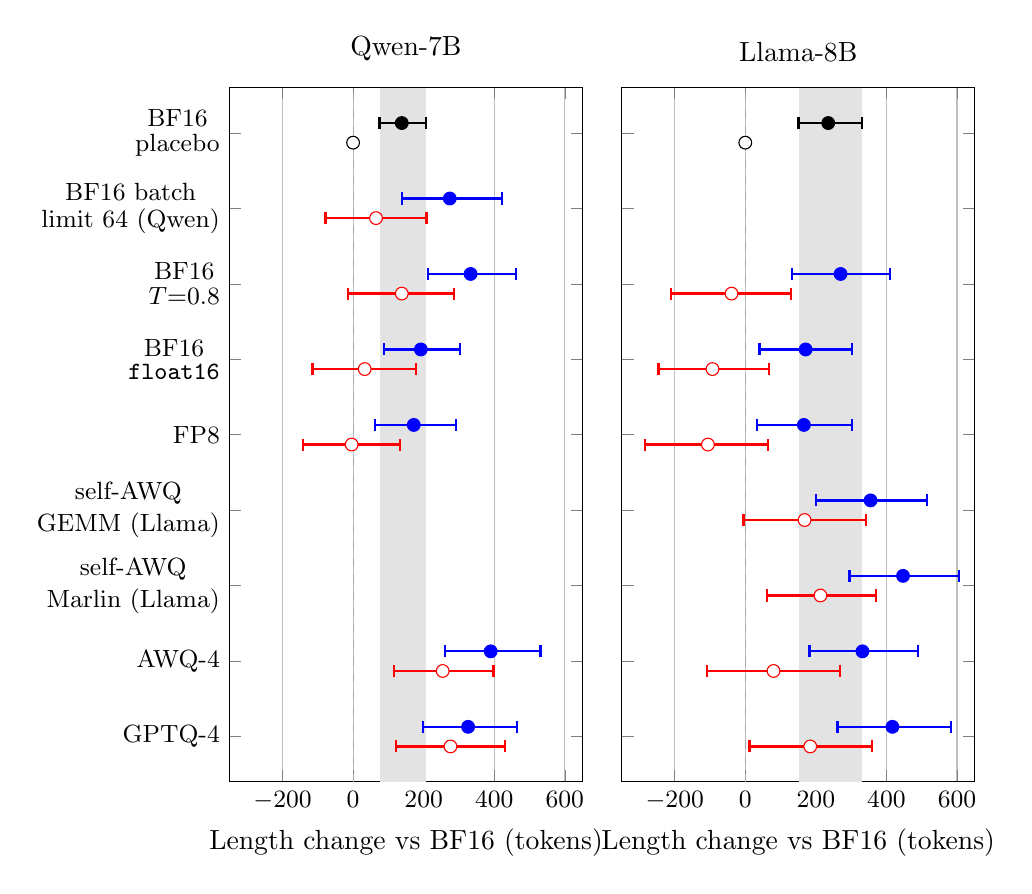
\begin{tikzpicture}
\begin{groupplot}[
    group style={group size=2 by 1, horizontal sep=0.5cm, yticklabels at=edge left},
    width=0.5\linewidth, height=10.4cm,
    xmin=-350, xmax=650, ymin=0.4, ymax=9.6,
    ytick={1,2,3,4,5,6,7,8,9}, yticklabels={GPTQ-4, AWQ-4, \shortstack{self-AWQ\\Marlin (Llama)}, \shortstack{self-AWQ\\GEMM (Llama)}, FP8, \shortstack{BF16\\\texttt{float16}}, \shortstack{BF16\\$T{=}0.8$}, \shortstack{BF16 batch\\limit 64 (Qwen)}, \shortstack{BF16\\placebo}},
    xlabel={Length change vs BF16 (tokens)},
    xmajorgrids=true,
    tick label style={font=\small},
]
\nextgroupplot[title={Qwen-7B}]
\fill[gray!22] (axis cs:75,0.4) rectangle (axis cs:207,9.6);
\draw[gray!70, dashed] (axis cs:0,0.4) -- (axis cs:0,9.6);
\draw[blue, thick] (axis cs:63,5.13) -- (axis cs:291,5.13);
\draw[blue, thick] (axis cs:63,5.05) -- (axis cs:63,5.21);
\draw[blue, thick] (axis cs:291,5.05) -- (axis cs:291,5.21);
\draw[red, thick] (axis cs:-142,4.87) -- (axis cs:134,4.87);
\draw[red, thick] (axis cs:-142,4.79) -- (axis cs:-142,4.95);
\draw[red, thick] (axis cs:134,4.79) -- (axis cs:134,4.95);
\draw[blue, thick] (axis cs:261,2.13) -- (axis cs:531,2.13);
\draw[blue, thick] (axis cs:261,2.05) -- (axis cs:261,2.21);
\draw[blue, thick] (axis cs:531,2.05) -- (axis cs:531,2.21);
\draw[red, thick] (axis cs:116,1.87) -- (axis cs:398,1.87);
\draw[red, thick] (axis cs:116,1.79) -- (axis cs:116,1.95);
\draw[red, thick] (axis cs:398,1.79) -- (axis cs:398,1.95);
\draw[blue, thick] (axis cs:198,1.13) -- (axis cs:464,1.13);
\draw[blue, thick] (axis cs:198,1.05) -- (axis cs:198,1.21);
\draw[blue, thick] (axis cs:464,1.05) -- (axis cs:464,1.21);
\draw[red, thick] (axis cs:121,0.87) -- (axis cs:431,0.87);
\draw[red, thick] (axis cs:121,0.79) -- (axis cs:121,0.95);
\draw[red, thick] (axis cs:431,0.79) -- (axis cs:431,0.95);
\draw[blue, thick] (axis cs:87,6.13) -- (axis cs:304,6.13);
\draw[blue, thick] (axis cs:87,6.05) -- (axis cs:87,6.21);
\draw[blue, thick] (axis cs:304,6.05) -- (axis cs:304,6.21);
\draw[red, thick] (axis cs:-115,5.87) -- (axis cs:178,5.87);
\draw[red, thick] (axis cs:-115,5.79) -- (axis cs:-115,5.95);
\draw[red, thick] (axis cs:178,5.79) -- (axis cs:178,5.95);
\draw[blue, thick] (axis cs:212,7.13) -- (axis cs:462,7.13);
\draw[blue, thick] (axis cs:212,7.05) -- (axis cs:212,7.21);
\draw[blue, thick] (axis cs:462,7.05) -- (axis cs:462,7.21);
\draw[red, thick] (axis cs:-15,6.87) -- (axis cs:286,6.87);
\draw[red, thick] (axis cs:-15,6.79) -- (axis cs:-15,6.95);
\draw[red, thick] (axis cs:286,6.79) -- (axis cs:286,6.95);
\draw[blue, thick] (axis cs:139,8.13) -- (axis cs:422,8.13);
\draw[blue, thick] (axis cs:139,8.05) -- (axis cs:139,8.21);
\draw[blue, thick] (axis cs:422,8.05) -- (axis cs:422,8.21);
\draw[red, thick] (axis cs:-78,7.87) -- (axis cs:208,7.87);
\draw[red, thick] (axis cs:-78,7.79) -- (axis cs:-78,7.95);
\draw[red, thick] (axis cs:208,7.79) -- (axis cs:208,7.95);
\draw[black, thick] (axis cs:75,9.13) -- (axis cs:207,9.13);
\draw[black, thick] (axis cs:75,9.05) -- (axis cs:75,9.21);
\draw[black, thick] (axis cs:207,9.05) -- (axis cs:207,9.21);
\addplot[only marks, mark=*, color=black, mark size=2.3pt] coordinates {(138,9.13)};
\addplot[only marks, mark=*, mark options={draw=black, fill=white}, mark size=2.3pt] coordinates {(0,8.87)};
\addplot[only marks, mark=*, color=blue, mark size=2.3pt] coordinates {(172,5.13) (390,2.13) (326,1.13) (192,6.13) (333,7.13) (274,8.13)};
\addplot[only marks, mark=*, mark options={draw=red, fill=white}, mark size=2.3pt] coordinates {(-4,4.87) (254,1.87) (276,0.87) (33,5.87) (138,6.87) (65,7.87)};
\nextgroupplot[title={Llama-8B}]
\fill[gray!22] (axis cs:151,0.4) rectangle (axis cs:331,9.6);
\draw[gray!70, dashed] (axis cs:0,0.4) -- (axis cs:0,9.6);
\draw[blue, thick] (axis cs:33,5.13) -- (axis cs:302,5.13);
\draw[blue, thick] (axis cs:33,5.05) -- (axis cs:33,5.21);
\draw[blue, thick] (axis cs:302,5.05) -- (axis cs:302,5.21);
\draw[red, thick] (axis cs:-284,4.87) -- (axis cs:65,4.87);
\draw[red, thick] (axis cs:-284,4.79) -- (axis cs:-284,4.95);
\draw[red, thick] (axis cs:65,4.79) -- (axis cs:65,4.95);
\draw[blue, thick] (axis cs:182,2.13) -- (axis cs:490,2.13);
\draw[blue, thick] (axis cs:182,2.05) -- (axis cs:182,2.21);
\draw[blue, thick] (axis cs:490,2.05) -- (axis cs:490,2.21);
\draw[red, thick] (axis cs:-109,1.87) -- (axis cs:268,1.87);
\draw[red, thick] (axis cs:-109,1.79) -- (axis cs:-109,1.95);
\draw[red, thick] (axis cs:268,1.79) -- (axis cs:268,1.95);
\draw[blue, thick] (axis cs:261,1.13) -- (axis cs:583,1.13);
\draw[blue, thick] (axis cs:261,1.05) -- (axis cs:261,1.21);
\draw[blue, thick] (axis cs:583,1.05) -- (axis cs:583,1.21);
\draw[red, thick] (axis cs:12,0.87) -- (axis cs:359,0.87);
\draw[red, thick] (axis cs:12,0.79) -- (axis cs:12,0.95);
\draw[red, thick] (axis cs:359,0.79) -- (axis cs:359,0.95);
\draw[blue, thick] (axis cs:40,6.13) -- (axis cs:303,6.13);
\draw[blue, thick] (axis cs:40,6.05) -- (axis cs:40,6.21);
\draw[blue, thick] (axis cs:303,6.05) -- (axis cs:303,6.21);
\draw[red, thick] (axis cs:-246,5.87) -- (axis cs:67,5.87);
\draw[red, thick] (axis cs:-246,5.79) -- (axis cs:-246,5.95);
\draw[red, thick] (axis cs:67,5.79) -- (axis cs:67,5.95);
\draw[blue, thick] (axis cs:133,7.13) -- (axis cs:409,7.13);
\draw[blue, thick] (axis cs:133,7.05) -- (axis cs:133,7.21);
\draw[blue, thick] (axis cs:409,7.05) -- (axis cs:409,7.21);
\draw[red, thick] (axis cs:-211,6.87) -- (axis cs:129,6.87);
\draw[red, thick] (axis cs:-211,6.79) -- (axis cs:-211,6.95);
\draw[red, thick] (axis cs:129,6.79) -- (axis cs:129,6.95);
\draw[blue, thick] (axis cs:295,3.13) -- (axis cs:605,3.13);
\draw[blue, thick] (axis cs:295,3.05) -- (axis cs:295,3.21);
\draw[blue, thick] (axis cs:605,3.05) -- (axis cs:605,3.21);
\draw[red, thick] (axis cs:61,2.87) -- (axis cs:370,2.87);
\draw[red, thick] (axis cs:61,2.79) -- (axis cs:61,2.95);
\draw[red, thick] (axis cs:370,2.79) -- (axis cs:370,2.95);
\draw[blue, thick] (axis cs:200,4.13) -- (axis cs:514,4.13);
\draw[blue, thick] (axis cs:200,4.05) -- (axis cs:200,4.21);
\draw[blue, thick] (axis cs:514,4.05) -- (axis cs:514,4.21);
\draw[red, thick] (axis cs:-5,3.87) -- (axis cs:342,3.87);
\draw[red, thick] (axis cs:-5,3.79) -- (axis cs:-5,3.95);
\draw[red, thick] (axis cs:342,3.79) -- (axis cs:342,3.95);
\draw[black, thick] (axis cs:151,9.13) -- (axis cs:331,9.13);
\draw[black, thick] (axis cs:151,9.05) -- (axis cs:151,9.21);
\draw[black, thick] (axis cs:331,9.05) -- (axis cs:331,9.21);
\addplot[only marks, mark=*, color=black, mark size=2.3pt] coordinates {(235,9.13)};
\addplot[only marks, mark=*, mark options={draw=black, fill=white}, mark size=2.3pt] coordinates {(0,8.87)};
\addplot[only marks, mark=*, color=blue, mark size=2.3pt] coordinates {(166,5.13) (332,2.13) (417,1.13) (171,6.13) (270,7.13) (447,3.13) (355,4.13)};
\addplot[only marks, mark=*, mark options={draw=red, fill=white}, mark size=2.3pt] coordinates {(-106,4.87) (80,1.87) (184,0.87) (-93,5.87) (-39,6.87) (213,2.87) (168,3.87)};
\end{groupplot}
\end{tikzpicture}

\caption{The BF16-correct conditional length change $\Lambda_b$ (filled; blue for quantized checkpoints, black for the placebo) and the unconditional mean paired change (open; red) on MATH-500, with item-level 95\% intervals. The shaded band is the seed-placebo interval: the conditional estimator applied to two BF16 seeds, where the true effect is zero. Every conditional estimate is positive, but both FP8 values lie inside the band although their unconditional changes are near zero or negative; three of the four 4-bit checkpoints exceed it (Table~\ref{tab:placebo}). The two rows above FP8 are controls with no quantization: the unmodified weights run at \texttt{float16}, which also lies inside the band, and the same weights sampled at $T=0.8$ (Section~\ref{sec:followup}; Table~\ref{tab:followup}). Self-AWQ is a Llama AWQ-4 checkpoint that we quantized ourselves, run on vLLM's AWQ-Marlin kernel (Marlin) and rerun on the GEMM kernel that the uploads use (GEMM). The batch-limit row (Qwen only) lowers the scheduler's \texttt{max\_num\_seqs} from 256 to 64.}
\label{fig:placebo}
\end{figure}

\section{Related Work}
\label{sec:related}
\paragraph{Quantized reasoning models.} GPTQ~\cite{frantar2022gptq} and AWQ~\cite{lin2023awq} were validated mainly on short-form benchmarks, and SmoothQuant~\cite{xiao2023smoothquant} targets activation quantization. QRM~\cite{liu2025qrm} evaluates DeepSeek-R1 distillations across weight, activation and KV-cache quantization and reports accuracy and mean length. Kurtic et al.~\cite{kurtic2025give} study vLLM serving efficiency across formats and batching regimes, report accuracy for R1-distill models on AIME-24, MATH-500 and GPQA-Diamond, and show that format recommendations change between synchronous decoding and continuous batching. Marchisio et al.~\cite{marchisio2024quant} find that automatic metrics understate the harm of quantization and that mathematical reasoning degrades most, and Dong et al.~\cite{acbench2025} benchmark GPTQ and AWQ models on agentic tasks. Lotfi et al.~\cite{lotfi2026overthinking}, Li et al.~\cite{li2025quantmeets}, Helcig et al.~\cite{helcig2026slq}, Zhong et al.~\cite{zhong2025quantized} and Ayadi et al.~\cite{ayadi2026reliability} study overthinking, reasoning degradation, statistically lossless quantization, calibration and reliability scaling; we do not re-estimate those quantities. Appendix Table~\ref{tab:related} compares designs.

\paragraph{Token inflation.} Lian et al.~\cite{lian2026quantinflates} report quantization-induced token inflation as a ratio of mean chain-of-thought lengths under greedy decoding (100 questions per benchmark) and, in a supplementary correctness-conditioned analysis (their Appendix~D.1, on Qwen3-30B), find inflation stronger on the BF16-correct subset. Our ratio-of-means estimand counts whole completions at $T=0.6$, so the two are related but not identical. A seed placebo needs stochastic sampling and cannot be run under greedy decoding; our selection-bias result therefore concerns the sampled setting and does not by itself bear on greedy estimates. Configuration changes such as batch size or GPU count do perturb greedy trajectories~\cite{yuan2025nondeterminism}, so a configuration placebo could play the same role under greedy decoding; we leave this to future work.

\paragraph{Reproducibility and nondeterminism.} Hochlehnert et al.~\cite{hochlehnert2025sober} show that seeds, prompts, decoding and software versions move reasoning scores. Yuan et al.~\cite{yuan2025nondeterminism} show that, with identical weights, changing the GPU count, GPU type or evaluation batch size changes both accuracy and response length of reasoning models, including R1-Distill-Qwen-7B in BF16, and trace this to floating-point non-associativity; they report the per-item spread of length across runtime configurations, but do not condition on correctness. Song et al.~\cite{song2025greedy} document the gap between greedy decoding and sampling and the variance across samples, and the notion of a background temperature~\cite{messina2026backgroundtemp} formalizes the randomness that remains at nominal $T=0$. Patodiya~\cite{patodiya2026cache} finds that, with model, decoding parameters, seed and request order fixed, enabling prefix caching changes agent trajectories on $36\%$ of episodes at 16-bit precision and on $75\%$ at four-bit, so quantization amplifies serving-induced divergence. Run-to-run reproducibility has also been studied for constrained classification outputs, where single runs are often sufficient~\cite{windisch2026onerun}; reasoning-trace length is a heavy-tailed quantity, and Section~\ref{sec:length} shows that the run-to-run component is large enough to dominate a conditional comparison. Our contribution is complementary: rather than varying the stack, we pin it and ask how much of an estimate is produced by the estimator itself. On statistical practice, Bowyer et al.~\cite{bowyer2025clt} show that CLT-based and bootstrap intervals can be poorly calibrated on small benchmarks; Appendix~\ref{app:prop-checks} compares four interval constructions on our 18 accuracy contrasts.

\paragraph{A/A tests, negative controls and selection.} The seed placebo applies a long-standing device. In online experimentation, A/A tests, in which both arms receive the same treatment, validate estimators and expose bias because the true effect is zero~\cite{kohavi2020trustworthy,guo2021mlrate,aadiag2016}; negative-control outcomes and exposures play the same role in epidemiology~\cite{lipsitch2010negative}. Like Guo et al.~\cite{guo2021mlrate}, we use cross-fitting to remove overfitting bias from a plug-in adjustment. What is specific to our setting is that correctness is a post-treatment variable: conditioning on it compares different sets of items across arms, the situation addressed by principal stratification and by work on selection bias~\cite{frangakis2002principal,zhang2003truncation,hernan2004selection}. Montgomery et al.~\cite{montgomery2018posttreatment} give the general warning for experiments. Zhang~\cite{zhang2026skill} derives a closely related decomposition for agent evaluation, in which a paired contrast restricted to runs where an event occurred contains a selection term that depends on whether the two arms are independent given the task or share a seed, and gives an analytic example in which the true effect is zero. Proposition~\ref{prop:placebo} is the analogue for correctness-conditioned length, and the seed placebo turns the null example into a measurement. To our knowledge, this control has not been applied to correctness-conditioned comparisons of language models; Proposition~\ref{prop:placebo} supplies the decomposition that explains what it measures. A related instance-level view appears in the study of accelerated vision-language models by Sun et al.~\cite{hiddeninstability2025}, who report the share of correct answers that become wrong after quantization or token reduction; Section~\ref{sec:generalise} supplies the missing same-model baseline for that statistic.

\section{Estimands and Diagnostics}
\label{sec:metrics}
\subsection{Notation and paired accuracy contrasts}
Let $i=1,\dots,n$ index benchmark items and $s\in S$ index generation seeds ($|S|=5$ on MATH-500 and $3$ elsewhere). For a checkpoint $m\in\{b,q\}$, where $b$ is the BF16 reference and $q$ a quantized checkpoint of the same family, $y^m_{is}\in\{0,1\}$ is extractive-match correctness and $\ell^m_{is}$ the completion length in tokens. The pass@1 contrast is $\Delta=n^{-1}\sum_i\delta_i$ with $\delta_i=\bar y^{q}_{i}-\bar y^{b}_{i}$, the difference of seed means on item $i$. We resample items ($B=10{,}000$), invert the percentile interval for a two-sided $p$-value, and apply Holm--Bonferroni within each benchmark's six format contrasts; a joint correction over all 18 contrasts is a stricter sensitivity. A two-way bootstrap that also resamples seeds checks that conclusions do not rest on the seeds that were run. Decisions within Monte Carlo error of $\alpha$ are rerun with $B=10^6$, a sign-flip permutation test and a paired $t$-test. Equivalence is assessed by TOST at $\pm1$\,pp and graded by Bayesian-bootstrap posterior probabilities. maj@5 counts an item correct when at least three of five seeds are correct. Appendix~\ref{app:stats} gives full details.

\subsection{Correctness-conditioned length and the seed placebo}
\label{sec:placebo-def}
Write $a_i=\Pr(y^b_{is}=1)$ and $c_i=\Pr(y^q_{is}=1)$ for per-item accuracies, $\mu^m_i=\mathbb{E}[\ell^m_{is}]$ for mean lengths, and $\mu^{m|1}_i$, $\mu^{m|0}_i$ for mean lengths of correct and incorrect completions. Our primary length estimands are unconditional: the ratio of means $\sum\ell^q/\sum\ell^b$ and the mean paired difference $\overline{\Delta\ell}=(n|S|)^{-1}\sum_{i,s}(\ell^q_{is}-\ell^b_{is})$. Following Lian et al.~\cite{lian2026quantinflates}, the \emph{BF16-correct} conditional and its mirror are
\begin{equation}
\Lambda_b=\frac{\sum_{i,s} y^b_{is}\,(\ell^q_{is}-\ell^b_{is})}{\sum_{i,s} y^b_{is}},\qquad
\Lambda_q=\frac{\sum_{i,s} y^q_{is}\,(\ell^q_{is}-\ell^b_{is})}{\sum_{i,s} y^q_{is}}.
\end{equation}
The \emph{seed placebo} applies $\Lambda_b$ to two seeds of the BF16 checkpoint, pooled over all $|S|(|S|-1)$ ordered seed pairs (20 on MATH-500):
\begin{equation}
\Pi_b=\frac{\sum_{i}\sum_{s\neq t} y^b_{is}\,(\ell^b_{it}-\ell^b_{is})}{\sum_{i}\sum_{s\neq t} y^b_{is}}.
\end{equation}
The same pooling gives the unconditional paired difference a placebo of exactly zero, and gives the mirrored estimator a placebo of exactly $-\Pi_b$.

\begin{proposition}[Placebo decomposition]
\label{prop:placebo}
Treat the items as fixed and suppose that, given the item, (A1) the runs of a checkpoint are independent and identically distributed across seeds, with correctness and length arbitrarily dependent within a run, and (A2) every BF16 run is independent of every quantized run. The numerator of each estimator below has exactly the stated expectation, and each ratio satisfies the stated relation up to $O(1/n)$, for completion lengths bounded by the output cap:
\begin{equation}
\mathbb{E}\,\Lambda_b = \Delta_a + S_b + O(1/n),\qquad \mathbb{E}\,\Pi_b = S_b + O(1/n),\qquad \mathbb{E}\,\Lambda_q = \Delta_c - S_q + O(1/n),
\end{equation}
where
\begin{equation}
\Delta_a=\frac{\sum_i a_i(\mu^q_i-\mu^b_i)}{\sum_i a_i},\qquad
S_b=\frac{\sum_i a_i(1-a_i)(\mu^{b|0}_i-\mu^{b|1}_i)}{\sum_i a_i},
\end{equation}
and $\Delta_c$, $S_q$ are defined in the same way with $c_i$ and the quantized lengths. The proof is in Appendix~\ref{app:proof}.
\end{proposition}

\begin{remark}[Exact form of the pooled placebo]
\label{rem:exact}
Let $k_i$ be the number of seeds in which BF16 solves item $i$ and $\hat\mu^{b|1}_i,\hat\mu^{b|0}_i$ the mean lengths of its correct and incorrect runs. Pooling over all ordered seed pairs gives, exactly,
\[
\Pi_b=\frac{\sum_i k_i(|S|-k_i)\,(\hat\mu^{b|0}_i-\hat\mu^{b|1}_i)}{(|S|-1)\sum_i k_i},
\]
which is $|S|/(|S|-1)$ times the plug-in value of $S_b$ with $a_i=k_i/|S|$. Because $\mathbb{E}[k_i(|S|-k_i)]=|S|(|S|-1)a_i(1-a_i)$, the numerator is unbiased for the numerator of $S_b$, so the pooled placebo is the natural estimator of $S_b$ (to the same ratio-estimator approximation as the proposition). The identity holds to machine precision on every BF16 cell (Appendix~\ref{app:prop-checks}). Cross-seed pairs need independence only across different seeds, so we recommend computing $\Lambda_b$ over cross-seed pairs; seed-matched pairs additionally require independence of the two checkpoints at the same seed and would bias $\Lambda_b-\Pi_b$ downward if the arms were coupled (Appendix Table~\ref{tab:sim}). In our data the two pairings differ by at most $29$ tokens and give the same set of checkpoints whose excess interval excludes zero (Appendix Table~\ref{tab:coupling}).
\end{remark}

Three consequences follow. First, the selection term $S_b$ is positive when failed BF16 traces are longer than correct ones on the items that BF16 solves only sometimes (exactly, when $\mu^{b|0}_i>\mu^{b|1}_i$ for those items, or on average with weights $a_i(1-a_i)$), and it vanishes on items that BF16 always or never solves; it comes only from items that BF16 solves in some but not all runs, which correctness conditioning cannot avoid; in our data about three quarters of it comes from items solved in three or four of five runs (Appendix Table~\ref{tab:share-k}). Second, the placebo needs no quantized run and can be estimated from the baseline seeds alone. Third, $\Lambda_b-\Pi_b$ estimates $\Delta_a$, the unconditional change reweighted towards items BF16 usually solves. This is a well-defined estimand but a different one from $\overline{\Delta\ell}$; it is a diagnostic contrast, not a corrected causal effect. The proposition conditions on the fixed item set of each benchmark; reading the item-level bootstrap intervals as inference about a population of similar items treats the items as exchangeable draws, an assumption we do not test. The two conditionals carry selection terms of opposite sign, which is why they disagree. A plug-in estimate of $\Delta_a$ that takes the weights and the length difference from the same BF16 seeds is biased upward, so we cross-fit: weights from four BF16 seeds, the difference from the held-out seed, averaged over five folds. Assumption (A2) can be probed: same-seed and cross-seed pairs of the two checkpoints agree on correctness at the same rate ($0.9536$ versus $0.9526$ for Qwen FP8 against BF16, with similar gaps in every contrast), and seed-matched and cross-seed $\Lambda_b$ differ by at most $29$ tokens with every interval including zero (Appendix Table~\ref{tab:coupling}). Both FP8 contrasts differ slightly in the direction that coupling would produce, so we cannot exclude mild coupling at the same seed; cross-seed pairs, which need independence only across different seeds, avoid the issue. A direct probe is available from Section~\ref{sec:followup}: two BF16 runs at the same seed that differ only in a scheduler setting are token-identical in $5$ of $2{,}500$ cases and diverge at a median of token $140$, so a shared seed does not keep differently computed runs together for long, which supports (A2) for seed-matched pairs of different checkpoints.

\section{Experimental Setup}
\label{sec:setup}
\subsection{Checkpoints and formats}
\label{sec:setup-models}
We evaluate DeepSeek-R1-Distill-Qwen-7B and DeepSeek-R1-Distill-Llama-8B~\cite{guo2025deepseekr1} in four formats: uncompressed BF16; RedHatAI FP8 checkpoints, which vLLM executes on the A100 as Marlin W8A16 weight-only kernels~\cite{frantar2024marlin} rather than native W8A8; RedHatAI GPTQ-4 (W4A16, group size 128, Marlin kernel); and community AWQ-4 uploads (group size 128). Hugging Face identifiers and revisions are in Appendix Table~\ref{tab:checkpoints}.

\paragraph{AWQ-4 denotes two specific artifacts.} The two \texttt{jakiAJK} AWQ-4 uploads differ from BF16 in more than their weights. They run with \texttt{float16} activations; they use vLLM's GEMM AWQ kernel, because their \texttt{zero\_point=false} configuration precludes the AWQ-Marlin conversion in vLLM~0.7.0; and their chat template omits the \texttt{<think>\textbackslash n} generation suffix, which the model then emits itself in all $14{,}102$ AWQ-4 completions, so the decoding context matches BF16 from the next token on. Their configuration metadata point to an AutoRound-style export with undocumented calibration. We therefore report the campaign AWQ-4 results as properties of these uploads, not of the AWQ algorithm, and test them separately on checkpoints that we quantized ourselves (Sections~\ref{sec:artifacts} and~\ref{sec:res1}). Appendix~\ref{app:provenance} gives the full provenance and Table~\ref{tab:dtype} the dtype and kernel of every format.

\subsection{Benchmarks and decoding}
MATH-500~\cite{hendrycks2021math,lightman2023lets} ($n=500$, seeds 42--46), GSM8K~\cite{cobbe2021gsm8k} ($n=1{,}319$, seeds 42--44) and GPQA-Diamond~\cite{rein2023gpqa} ($n=198$, seeds 42--44) give 88 campaign runs (checkpoint$\times$benchmark$\times$seed) and $56{,}408$ completions; the follow-up experiments of Sections~\ref{sec:followup}--\ref{sec:res1} add $48$ cells from our own runs and $87$ cells from companion studies (Appendix~\ref{app:followup}). Prompts follow the QRM template (Appendix~\ref{sec:prompt}). Decoding uses $T=0.6$, top-$p=0.95$, repetition penalty $1.0$ (deliberately not used to hide loops) and a 32{,}768-token budget; because vLLM bounds prompt plus output, the effective output cap is $31{,}957$--$32{,}743$ tokens depending on the item. Native stop reasons were not logged in the campaign, so a completion counts as \emph{truncated} when it lies within 16 tokens of its per-item cap ($147$ of the $155$ such MATH-500 rows are exactly at the cap), and as a \emph{loop} when it contains a run of at least 20 identical words (Appendix~\ref{sec:pathology}). The stored prompts show that GPQA-Diamond answer order is identical across all checkpoints and seeds, so GPQA contrasts are paired.

\subsection{Serving stack}
All runs use the PARAM Rudra HPC system (NVIDIA A100-PCIE-80GB) with vLLM~0.7.0, \texttt{enforce\_eager=true} and \texttt{gpu\_memory\_utilization=0.75}, through QRM's \texttt{inference.py}. Eager execution keeps the accuracy path reproducible but adds kernel-launch overhead on single-stream decode; we ran no CUDA-graph replicate. Serving-time measurements are reported in Appendix~\ref{app:secondary}.

\section{Results}
\label{sec:results}
\subsection{Much of the correctness-conditioned length change is selection}
\label{sec:length}
\paragraph{Unconditional changes.} On the full MATH-500 grid, the Qwen AWQ-4 and GPTQ-4 checkpoints produce $6.3\%$ and $6.9\%$ more tokens than BF16 (mean paired differences $+254$ and $+276$, intervals excluding zero) and Llama GPTQ-4 $3.9\%$ more ($+184$). Llama AWQ-4 ($+1.7\%$) and both FP8 checkpoints have intervals that include zero (Table~\ref{tab:placebo}, first column).

\paragraph{The conditional estimator.} The BF16-correct conditional $\Lambda_b$ is positive with an interval excluding zero in all six contrasts ($+166$ to $+417$), including Qwen FP8, whose unconditional change is $-4$ $[-142,+134]$. The mechanism is visible in the correctness strata. Failed traces are far longer than correct ones ($15{,}843$ versus $3{,}256$ tokens for Qwen BF16; $13{,}928$ versus $3{,}539$ for Llama BF16), and $\Lambda_b$ mixes the jointly correct pairs with the pairs in which only BF16 is correct, where the quantized trace is a failure: for Qwen FP8, $(2297\times 51+53\times 5444)/2350\approx 172$ (Appendix Table~\ref{tab:tokens}). The mirrored $\Lambda_q$ mixes in BF16's failures instead, and its point estimate is negative in four of six contrasts, three with intervals excluding zero.

\paragraph{The placebo.} Applying $\Lambda_b$ to two BF16 seeds gives $+138$ $[+75,+207]$ tokens for Qwen and $+235$ $[+151,+331]$ for Llama, with no quantization at all. Both FP8 conditionals ($+172$, $+166$) lie inside their family's placebo interval, and their paired excess over the placebo is $+35$ $[-82,+158]$ and $-70$ $[-219,+74]$: we detect no FP8 length change beyond selection, which is an absence of evidence rather than evidence of equality. Three 4-bit checkpoints exceed the placebo with intervals excluding zero: Qwen AWQ-4 ($+252$), Qwen GPTQ-4 ($+188$) and Llama GPTQ-4 ($+182$). Llama AWQ-4 does not ($+97$ $[-66,+267]$). The cross-fitted reweighted change $\Delta_a$, which Proposition~\ref{prop:placebo} says the excess estimates, is close to the excess in every contrast (Table~\ref{tab:placebo}, last two columns), a consistency check on the independence assumption. It is close to the unconditional difference for Qwen AWQ-4 ($+236$ versus $+254$) but smaller for Qwen GPTQ-4 ($+197$ versus $+276$), whose extra length falls disproportionately on items that BF16 often fails. Computing $\Lambda_b$ over cross-seed pairs, as we recommend, changes each estimate by at most $29$ tokens and leaves unchanged the set of checkpoints whose excess interval excludes zero (Appendix Table~\ref{tab:coupling}). Sections~\ref{sec:followup} and~\ref{sec:artifacts} test whether the placebo and these excesses depend on the seeds, on the numeric format or on the particular checkpoint.

\begin{table}[t]
\centering
\caption{MATH-500 length change versus BF16 (tokens), all five seeds, with item-level 95\% intervals ($B=10{,}000$). Placebo rows apply each estimator to BF16 seed $s$ against BF16 seed $t\neq s$, pooled over 20 ordered pairs; by construction the unconditional placebo is exactly zero and the quant-correct placebo is exactly the negative of the BF16-correct one. Excess: $\Lambda_b-\Pi_b$ on shared item resamples. Cross-fit $\widehat\Delta_a$: accuracy-weighted unconditional change, with weights from four BF16 seeds and the difference from the held-out seed, averaged over five folds (Section~\ref{sec:placebo-def}). Correctness strata are in Appendix Table~\ref{tab:tokens}.}
\label{tab:placebo}
\small
\resizebox{\linewidth}{!}{%
\begin{tabular}{lccccc}
\toprule
\textbf{Contrast} & \vcell{\textbf{Unconditional}}{$\overline{\Delta\ell}$} & \vcell{\textbf{BF16-correct}}{$\Lambda_b$} & \vcell{\textbf{Quant-correct}}{$\Lambda_q$} & \vcell{\textbf{Excess}}{$\Lambda_b-\Pi_b$} & \vcell{\textbf{Cross-fit}}{$\widehat\Delta_a$} \\
\midrule
Qwen BF16 vs BF16 (placebo) & \vcell{$0$}{(exact)} & \vcell{$+138$}{$[+75,+207]$} & \vcell{$-138$}{(exact)} & --- & --- \\
Qwen FP8 & \vcell{$-4$}{$[-142,+134]$} & \vcell{$+172$}{$[+63,+291]$} & \vcell{$-136$}{$[-273,-3]$} & \vcell{$+35$}{$[-82,+158]$} & \vcell{$+55$}{$[-58,+171]$} \\
Qwen AWQ-4 & \vcell{$+254$}{$[+116,+398]$} & \vcell{$+390$}{$[+261,+531]$} & \vcell{$+5$}{$[-111,+114]$} & \vcell{$+252$}{$[+136,+380]$} & \vcell{$+236$}{$[+118,+361]$} \\
Qwen GPTQ-4 & \vcell{$+276$}{$[+121,+431]$} & \vcell{$+326$}{$[+198,+464]$} & \vcell{$+22$}{$[-99,+151]$} & \vcell{$+188$}{$[+49,+335]$} & \vcell{$+197$}{$[+72,+332]$} \\
\midrule
Llama BF16 vs BF16 (placebo) & \vcell{$0$}{(exact)} & \vcell{$+235$}{$[+151,+331]$} & \vcell{$-235$}{(exact)} & --- & --- \\
Llama FP8 & \vcell{$-106$}{$[-284,+65]$} & \vcell{$+166$}{$[+33,+302]$} & \vcell{$-182$}{$[-339,-35]$} & \vcell{$-70$}{$[-219,+74]$} & \vcell{$-41$}{$[-186,+100]$} \\
Llama AWQ-4 & \vcell{$+80$}{$[-109,+268]$} & \vcell{$+332$}{$[+182,+490]$} & \vcell{$-141$}{$[-303,+12]$} & \vcell{$+97$}{$[-66,+267]$} & \vcell{$+115$}{$[-44,+281]$} \\
Llama GPTQ-4 & \vcell{$+184$}{$[+12,+359]$} & \vcell{$+417$}{$[+261,+583]$} & \vcell{$-183$}{$[-335,-35]$} & \vcell{$+182$}{$[+25,+344]$} & \vcell{$+160$}{$[+10,+312]$} \\
\bottomrule
\end{tabular}%
}
\end{table}

\paragraph{Where the extra length goes.} Mean differences are carried by a minority of very long traces (Table~\ref{tab:toklocation}). Qwen AWQ-4 and GPTQ-4 have median per-item differences of $+50$ and $+4$ tokens, against means of $+254$ and $+276$, and every Llama median has an interval that includes zero. A mean-based inflation figure and a typical-trace figure therefore answer different questions, and both should be reported. Keyword counts of self-checking phrases are higher in the longer Qwen 4-bit and Llama GPTQ-4 traces even among finished completions, but not in Llama AWQ-4 (Appendix Table~\ref{tab:reflection}); these are keyword counts, not an analysis of reasoning quality.

\begin{table}[t]
\centering
\caption{MATH-500 paired token difference (quantized $-$ BF16) of the seed-averaged per-item delta: mean, median, and 10\%-trimmed mean, each with an item-level 95\% CI ($B=10{,}000$). The means reproduce Table~\ref{tab:tokens} up to Monte Carlo error.}
\label{tab:toklocation}
\small
\begin{tabular}{llll}
\toprule
\textbf{Contrast} & \textbf{Mean} & \textbf{Median} & \textbf{10\%-trimmed mean} \\
\midrule
Qwen FP8 & $-4$ $[-144,+137]$ & $0$ $[-33,+48]$ & $+30$ $[-34,+92]$ \\
Qwen AWQ-4 & $+254$ $[+116,+394]$ & $+50$ $[+10,+92]$ & $+118$ $[+49,+192]$ \\
Qwen GPTQ-4 & $+276$ $[+123,+433]$ & $+4$ $[-43,+56]$ & $+92$ $[+27,+169]$ \\
\midrule
Llama FP8 & $-106$ $[-278,+67]$ & $-29$ $[-105,+9]$ & $-57$ $[-148,+32]$ \\
Llama AWQ-4 & $+80$ $[-110,+270]$ & $+11$ $[-61,+83]$ & $+79$ $[-26,+183]$ \\
Llama GPTQ-4 & $+184$ $[+11,+359]$ & $+38$ $[-19,+116]$ & $+90$ $[-20,+205]$ \\
\bottomrule
\end{tabular}
\end{table}

\subsection{The placebo beyond MATH-500 length: other benchmarks and answer flips}
\label{sec:generalise}
\paragraph{Other benchmarks.} Table~\ref{tab:crossbench} applies the placebo to GSM8K and GPQA-Diamond. It is positive in both families on all three benchmarks, with intervals excluding zero in five of six cells (Llama on GPQA-Diamond, with three seeds and $n=198$, includes zero), and it is $2$--$5\%$ of the mean completion length in every cell. GPQA-Diamond has by far the largest share of intermediate items ($40$--$41\%$, against $10$--$21\%$ on MATH-500 and $7$--$11\%$ on GSM8K) but its failed traces are only $1.3$--$1.4$ times as long as its correct ones, against $2.3$--$2.4$ on GSM8K and $3.9$--$4.9$ on MATH-500 (global means). Proposition~\ref{prop:placebo} implies exactly this trade-off: the selection term scales with the product of the share of intermediate items and the failed-versus-correct length gap, so a benchmark with more intermediate items need not have a larger placebo.

\begin{table}[t]
\centering
\caption{The seed placebo $\Pi_b$ on every benchmark (BF16 seed against another BF16 seed, pooled over all ordered seed pairs; item-level 95\% intervals, $B=10{,}000$). ``Intermediate'' is the share of items that BF16 solves in at least one but not all seeds, the only items that can contribute to $S_b$. The last column expresses the placebo as a percentage of the mean completion length. GPQA-Diamond has $n=198$ and three seeds, hence the wide intervals.}
\label{tab:crossbench}
\small
\begin{tabular}{llcccc}
\toprule
\textbf{Benchmark} & \textbf{Family} & \textbf{Acc.\ (\%)} & \textbf{Intermediate (\%)} & \textbf{Placebo $\Pi_b$ (tokens)} & \textbf{\% of mean length} \\
\midrule
MATH-500 (5 seeds) & Qwen-7B & $94.0$ & $9.6$ & $+138$ $[+75,+207]$ & $3.4$ \\
 & Llama-8B & $89.2$ & $21.4$ & $+235$ $[+151,+331]$ & $5.1$ \\
\midrule
GSM8K (3 seeds) & Qwen-7B & $91.3$ & $6.6$ & $+58$ $[+26,+97]$ & $3.4$ \\
 & Llama-8B & $88.7$ & $11.3$ & $+44$ $[+21,+68]$ & $2.5$ \\
\midrule
GPQA-D (3 seeds) & Qwen-7B & $50.3$ & $39.9$ & $+373$ $[+97,+677]$ & $4.4$ \\
 & Llama-8B & $46.1$ & $40.9$ & $+189$ $[-49,+481]$ & $2.2$ \\
\bottomrule
\end{tabular}
\end{table}


\paragraph{Answer flips.} The same logic applies to correct-to-wrong flips, which are sometimes read as a stability cost of quantization~\cite{hiddeninstability2025}. Two seeds of the unmodified BF16 model already flip a correct answer to a wrong one in $2.3\%$ (Qwen) and $5.0\%$ (Llama) of MATH-500 item-seed pairs, $2.2\%$ and $3.8\%$ on GSM8K, and about $13\%$ on GPQA-Diamond (Table~\ref{tab:flips}). Relative to this same-model baseline, only three of 18 excesses are detectable: Llama AWQ-4 on MATH-500 ($+2.18$\,pp $[+1.04,+3.37]$) and GSM8K ($+1.26$ $[+0.40,+2.12]$), and Qwen AWQ-4 on MATH-500 ($+0.85$ $[+0.13,+1.61]$). The other fifteen intervals include zero. This agrees with the accuracy results of Section~\ref{sec:res1} and shows that a raw flip rate of a few percent does not by itself indicate degradation. The 18 intervals are exploratory and not multiplicity-adjusted.

\begin{table}[t]
\centering
\caption{Correct-to-wrong flips with a same-model baseline. The flip rate is the share of (item, seed-pair) cases in which the reference run is correct and the other run is wrong. The placebo column pairs two BF16 seeds; the other columns give the excess over the placebo for each quantized checkpoint (cross-seed pairs, percentage points of items, item-level 95\% intervals). Bold: interval excludes zero. These 18 intervals are exploratory and not multiplicity-adjusted.}
\label{tab:flips}
\small
\resizebox{\linewidth}{!}{%
\begin{tabular}{llcccc}
\toprule
\textbf{Benchmark} & \textbf{Family} & \textbf{Placebo flips (pp)} & \textbf{FP8 excess} & \textbf{AWQ-4 excess} & \textbf{GPTQ-4 excess} \\
\midrule
MATH-500 (5 seeds) & Qwen-7B & $2.28$ & $-0.11$ $[-0.70,+0.51]$ & \textbf{$+0.85$ $[+0.13,+1.61]$} & $+0.48$ $[-0.17,+1.17]$ \\
 & Llama-8B & $5.00$ & $-0.50$ $[-1.41,+0.42]$ & \textbf{$+2.18$ $[+1.04,+3.37]$} & $+0.27$ $[-0.70,+1.26]$ \\
\midrule
GSM8K (3 seeds) & Qwen-7B & $2.20$ & $+0.14$ $[-0.39,+0.68]$ & $+0.29$ $[-0.28,+0.88]$ & $+0.43$ $[-0.15,+1.01]$ \\
 & Llama-8B & $3.77$ & $-0.06$ $[-0.71,+0.57]$ & \textbf{$+1.26$ $[+0.40,+2.12]$} & $-0.11$ $[-0.73,+0.53]$ \\
\midrule
GPQA-D (3 seeds) & Qwen-7B & $13.30$ & $-0.08$ $[-2.53,+2.36]$ & $+2.19$ $[-0.59,+4.97]$ & $+1.18$ $[-1.60,+4.04]$ \\
 & Llama-8B & $13.64$ & $-1.09$ $[-3.62,+1.52]$ & $+0.25$ $[-2.44,+2.95]$ & $+0.76$ $[-2.10,+3.54]$ \\
\bottomrule
\end{tabular}%
}
\end{table}


\subsection{Four further ways to produce the placebo}
\label{sec:followup}
The placebo above is estimated on the same five seeds as the quantized contrasts, and the argument that it reflects selection rather than quantization has so far rested on the BF16 baseline alone. Four additional experiments on the same stack and prompts test it (Table~\ref{tab:followup}; protocol and gates in Appendix~\ref{app:followup}), and a pilot grid from a companion study adds larger real changes to the sampling setting (Appendix Table~\ref{tab:p4ctrl}).

\paragraph{Precision alone.} In the accuracy campaign the AWQ-4 uploads run with \texttt{float16} activations whereas BF16, FP8 and GPTQ-4 do not, so precision is confounded with format. We therefore ran the unmodified BF16 weights at \texttt{float16} (five seeds, both families). Accuracy does not change (Qwen $+0.36$\,pp $[-0.48,+1.24]$; Llama $+0.28$ $[-0.80,+1.40]$) and neither does the unconditional length ($+33$ $[-115,+178]$ and $-93$ $[-246,+67]$ tokens). The BF16-correct estimator nevertheless reports $+192$ $[+87,+304]$ (Qwen) and $+171$ $[+40,+303]$ (Llama) tokens, with excess over the placebo of $+54$ $[-57,+170]$ and $-64$ $[-204,+70]$. A change that involves no quantization therefore produces apparent inflation similar to that of the two FP8 checkpoints ($+172$ and $+166$), as the placebo predicts, and it also shows that \texttt{float16} activations cannot by themselves account for the Llama AWQ-4 accuracy loss.

\paragraph{Temperature.} Sampling the same BF16 weights at $T=0.8$ instead of $0.6$ changes the sampling distribution, so, unlike the dtype control above, a nonzero excess is possible. The rule we fixed in advance was that a positive $\Lambda_b$ with a null excess indicates that the placebo generalizes beyond quantization. It holds for Llama ($\Lambda_b=+270$ $[+133,+409]$, excess $+35$ $[-113,+177]$, accuracy $+0.80$\,pp $[-0.40,+2.00]$) and does not hold for Qwen ($\Lambda_b=+333$ $[+212,+462]$, excess $+195$ $[+67,+324]$), where accuracy is unchanged ($+0.28$\,pp $[-0.64,+1.20]$) and the unconditional change is $+138$ $[-15,+286]$. We read the Qwen excess as a length change among items that BF16 solves, but we did not pre-register that reading and we did not test it further. The two families disagree, so the experiment supports the placebo for one family and shows that the excess can be nonzero for the other when a real change is made.

\paragraph{Larger changes to the sampling setting.} A pilot grid of decoding settings (Qwen BF16, 300 MATH-500 items, three seeds; Appendix Table~\ref{tab:p4ctrl}) provides larger real changes against the same reference. Lowering the temperature to $0.2$ gives an excess of $+1{,}070$ $[+591,+1{,}596]$ tokens with accuracy $-4.56$\,pp, and $8.6\%$ of completions stop at the length limit against under $1\%$ at $T=0.6$ and none at $T=1.0$, which points to repetition loops. Raising it to $1.0$ gives $+263$ $[+86,+435]$, and an $8{,}192$-token budget gives $-406$ $[-613,-217]$. A self-quantized AWQ-4 checkpoint at the campaign setting has an excess of $-117$ $[-307,+76]$ (its prompts lack the campaign's doubled beginning-of-sequence token; the BF16 cells use the campaign's prompts). Real changes to the sampling setting thus separate from the placebo by hundreds to a thousand tokens in both directions, so subtracting the placebo does not erase them; we did not test greedy decoding.

\paragraph{Batch limit alone.} Yuan et al.\ show that the evaluation batch size changes reasoning traces even when the weights are identical. We lowered the vLLM scheduler limit \texttt{max\_num\_seqs} from 256 to 64 for Qwen BF16, with the same prompts and sampling seeds. Only $5$ of $2{,}500$ completions are token-identical to the campaign runs, and the median first divergence is at token $140$ ($37\%$ of completions diverge within the first $100$ tokens), so a scheduler setting that does not touch the model rewrites the traces. Accuracy does not change ($-0.32$\,pp $[-1.12,+0.48]$) and neither does the unconditional length ($+65$ $[-78,+208]$ tokens). The BF16-correct estimator over cross-seed pairs reports $+248$ $[+128,+381]$ tokens; its excess over the placebo is $+111$ $[-14,+241]$, so by the rule fixed in advance the batch limit behaves like a change of seed. The point estimate is large relative to the placebo ($+138$) and seed-matched pairs give an excess of $+136$ $[+2,+274]$, which only just excludes zero, so we do not claim that a batch-limit change is a null. The correct-to-wrong flip rate exceeds the same-model baseline by $+0.34$\,pp $[-0.36,+1.07]$.

\paragraph{Held-out seeds.} The placebo could in principle be specific to the five seeds on which it was estimated. We generated five new BF16 seeds (47--51) for both families and compared the new placebo with the campaign placebo using a paired item bootstrap (Table~\ref{tab:x1}). The difference is $+61$ $[-24,+145]$ tokens for Qwen and $+7$ $[-97,+113]$ for Llama, so the pre-registered rule (the interval contains zero for both families) is met. The test can exclude only differences larger than roughly $85$--$105$ tokens, and the new Qwen placebo is higher in point estimate ($+199$ against $+138$). Pooled over all ten seeds the placebo is $+182$ $[+118,+252]$ for Qwen and $+232$ $[+168,+304]$ for Llama. Using this pooled placebo leaves each conclusion above unchanged: the seed-matched excess is $-10$ $[-134,+116]$ (Qwen FP8), $-67$ $[-211,+74]$ (Llama FP8), $+208$ $[+92,+336]$ (Qwen AWQ-4), $+144$ $[+17,+280]$ (Qwen GPTQ-4), $+185$ $[+35,+340]$ (Llama GPTQ-4) and $+100$ $[-54,+257]$ (Llama AWQ-4). Items solved in three or four of five seeds supply $81\%$ (Qwen) and $75\%$ (Llama) of the selection term on the new seeds, against $77\%$ and $75\%$ on the campaign seeds.

% generated by analysis/gen_followup_tables.py -- do not edit by hand
\begin{table}[t]
\centering
\caption{Follow-up contrasts against the campaign BF16 cells (tokens; item-level 95\% intervals, $B=10{,}000$). E2: the BF16 weights run at \texttt{float16}. E3: BF16 sampled at $T=0.8$ instead of $0.6$. E1: a Llama AWQ-4 checkpoint that we quantized ourselves (AutoAWQ, 4-bit, group size 128, \texttt{zero\_point=True}). The last two rows repeat the community AWQ-4 upload for reference. $\Lambda_b$: BF16-correct conditional change over seed-matched pairs (the convention of Table~\ref{tab:placebo}); $\Pi_b$: pooled seed placebo from the five campaign BF16 seeds ($+138$ and $+235$ on MATH-500, $+44$ on GSM8K for Llama); excess $=\Lambda_b-\Pi_b$ on shared item resamples. MATH-500 uses five seeds, GSM8K three. E1, E2 and E3 share the campaign prompts and sampling seeds; all 38 follow-up cells are recorded as passing the checks of Appendix~\ref{app:followup}.}
\label{tab:followup}
\small
\resizebox{\linewidth}{!}{%
\begin{tabular}{lccccc}
\toprule
\textbf{Contrast} & \vcell{\textbf{pass@1}}{$\Delta$ (pp)} & \vcell{\textbf{Unconditional}}{$\overline{\Delta\ell}$} & \vcell{\textbf{BF16-correct}}{$\Lambda_b$} & \vcell{\textbf{Placebo}}{$\Pi_b$} & \vcell{\textbf{Excess}}{$\Lambda_b-\Pi_b$} \\
\midrule
E2 Qwen, BF16 $\to$ \texttt{float16} & \vcell{$+0.36$}{$[-0.48,+1.24]$} & \vcell{$+33$}{$[-115,+178]$} & \vcell{$+192$}{$[+87,+304]$} & \vcell{$+138$}{$[+75,+207]$} & \vcell{$+54$}{$[-57,+170]$} \\
E2 Llama, BF16 $\to$ \texttt{float16} & \vcell{$+0.28$}{$[-0.80,+1.40]$} & \vcell{$-93$}{$[-246,+67]$} & \vcell{$+171$}{$[+40,+303]$} & \vcell{$+235$}{$[+151,+331]$} & \vcell{$-64$}{$[-204,+70]$} \\
\midrule
E3 Qwen, $T=0.8$ vs $0.6$ & \vcell{$+0.28$}{$[-0.64,+1.20]$} & \vcell{$+138$}{$[-15,+286]$} & \vcell{$+333$}{$[+212,+462]$} & \vcell{$+138$}{$[+75,+207]$} & \vcell{$+195$}{$[+67,+324]$} \\
E3 Llama, $T=0.8$ vs $0.6$ & \vcell{$+0.80$}{$[-0.40,+2.00]$} & \vcell{$-39$}{$[-211,+129]$} & \vcell{$+270$}{$[+133,+409]$} & \vcell{$+235$}{$[+151,+331]$} & \vcell{$+35$}{$[-113,+177]$} \\
\midrule
E1 Llama self-AWQ, MATH-500 & \vcell{$-1.68$}{$[-2.96,-0.40]$} & \vcell{$+213$}{$[+61,+370]$} & \vcell{$+447$}{$[+295,+605]$} & \vcell{$+235$}{$[+151,+331]$} & \vcell{$+211$}{$[+60,+362]$} \\
E1 Llama self-AWQ, GSM8K & \vcell{$-1.57$}{$[-2.53,-0.63]$} & \vcell{$+30$}{$[-32,+92]$} & \vcell{$+84$}{$[+28,+142]$} & \vcell{$+44$}{$[+21,+68]$} & \vcell{$+41$}{$[-18,+100]$} \\
Llama community AWQ-4, MATH-500 & \vcell{$-2.76$}{$[-4.16,-1.40]$} & \vcell{$+80$}{$[-111,+273]$} & \vcell{$+332$}{$[+180,+490]$} & \vcell{$+235$}{$[+151,+331]$} & \vcell{$+97$}{$[-62,+257]$} \\
Llama community AWQ-4, GSM8K & \vcell{$-1.57$}{$[-2.55,-0.61]$} & \vcell{$-16$}{$[-84,+54]$} & \vcell{$+14$}{$[-47,+78]$} & \vcell{$+44$}{$[+21,+68]$} & \vcell{$-29$}{$[-93,+36]$} \\
\bottomrule
\end{tabular}%
}
\end{table}


% generated by analysis/gen_followup_tables.py -- do not edit by hand
\begin{table}[t]
\centering
\caption{Held-out seeds (X1). The BF16 placebo $\Pi_b$ on MATH-500 from the five campaign seeds (42--46), from five new BF16 seeds (47--51; 20 ordered pairs each), their paired difference (same item resamples), and the placebo pooled over all ten seeds (90 ordered pairs). Item-level 95\% intervals, $B=10{,}000$. The pre-registered rule was that the interval of the paired difference contains zero for both families.}
\label{tab:x1}
\small
\resizebox{\linewidth}{!}{%
\begin{tabular}{lccccc}
\toprule
\textbf{Family} & \vcell{\textbf{Seeds 42--46}}{$\Pi_b$} & \vcell{\textbf{Seeds 47--51}}{$\Pi_b$} & \vcell{\textbf{Difference}}{new $-$ old} & \vcell{\textbf{All ten seeds}}{$\Pi_b$} & \textbf{Rule} \\
\midrule
Qwen & \vcell{$+138$}{$[+76,+211]$} & \vcell{$+199$}{$[+116,+293]$} & \vcell{$+61$}{$[-24,+145]$} & \vcell{$+182$}{$[+118,+252]$} & interval contains 0 \\
Llama & \vcell{$+235$}{$[+150,+331]$} & \vcell{$+243$}{$[+158,+337]$} & \vcell{$+7$}{$[-97,+113]$} & \vcell{$+232$}{$[+168,+304]$} & interval contains 0 \\
\bottomrule
\end{tabular}%
}
\end{table}


\subsection{Independent quantizations: the excess depends on the artifact}
\label{sec:artifacts}
The campaign evaluates one public checkpoint per format and family, so an excess could belong to a checkpoint and not to its method. A separate study on the same stack produced Qwen-7B checkpoints that we quantized ourselves: three independent calibration draws for each of GPTQ-4 (\texttt{bfloat16}, Marlin kernel) and AWQ-4 (\texttt{float16}, GEMM kernel), run on MATH-500 and GSM8K with seeds 42--44 and scored with the campaign scorer (Table~\ref{tab:p2qwen}; Appendix~\ref{app:followup}).

On MATH-500, for GPTQ-4 the excess over the five-seed placebo excludes zero in every draw ($+378$ $[+193,+579]$, $+415$ $[+229,+614]$, $+195$ $[+36,+370]$; pooled $+330$ $[+192,+479]$), larger than the community checkpoint's $+200$ $[+35,+373]$ on the same three seeds. For AWQ-4 it excludes zero in none ($-110$ $[-252,+33]$, $+100$ $[-82,+290]$, $-11$ $[-186,+171]$; pooled $-7$ $[-135,+124]$), although the community AWQ-4 gives $+155$ $[+17,+292]$ on the same seeds. Accuracy is similar to the community checkpoints' (pooled $-1.16$\,pp $[-2.13,-0.18]$ for GPTQ-4 and $-0.87$ $[-1.80,+0.07]$ for AWQ-4). Draws of the same method also differ from each other: two AWQ-4 draws differ by $-275$ tokens $[-459,-95]$ in mean length and two GPTQ-4 draws by $+215$ $[+11,+420]$, and accuracy differs between draws by up to $0.9$\,pp (intervals include zero). Running the GPTQ-4 draws at \texttt{float16} instead of \texttt{bfloat16} changes neither accuracy ($-1.00$ to $+0.07$\,pp) nor length ($-61$ to $+156$ tokens) detectably.

On GSM8K the picture agrees for GPTQ-4 and differs for AWQ-4 (placebo $+58$ $[+26,+97]$). The GPTQ-4 excess is positive in every draw ($+132$ $[+59,+206]$, $+92$ $[+18,+168]$, $+54$ $[-9,+115]$; pooled $+93$ $[+34,+149]$), where the community GPTQ-4 is at $+1$ $[-73,+77]$. The AWQ-4 excess is negative in every draw ($-192$ $[-264,-118]$, $-128$ $[-208,-44]$, $-171$ $[-248,-91]$; pooled $-164$ $[-228,-99]$): these traces are shorter than BF16's by $138$ tokens $[69,207]$ on average, whereas the community AWQ-4 is at $-35$ $[-99,+31]$. Accuracy stays within $0.5$\,pp of BF16 for both methods (pooled $-0.19$ $[-0.70,+0.35]$ and $-0.48$ $[-1.10,+0.13]$), draws differ in mean length by up to $105$ tokens (AWQ-4 draws 0 and 1: $-105$ $[-193,-22]$), and \texttt{float16} against \texttt{bfloat16} for GPTQ-4 is again indistinguishable ($-66$ to $+17$ tokens).

The length excess is therefore not a fixed property of a format. On MATH-500 it is present in all three GPTQ-4 draws and absent from all three AWQ-4 draws; on GSM8K it is positive for GPTQ-4 and negative for AWQ-4; and it varies by about $200$ tokens (MATH-500) and $100$ tokens (GSM8K) across draws of the same method. A single checkpoint per format cannot separate a method effect from an artifact effect, in addition to the selection effect that the placebo measures. One caveat applies to the contrast with campaign BF16 but not to the comparisons among the self-quantized rows: the prompts of these runs have one token fewer than the campaign's on every MATH-500 item (a single beginning-of-sequence token, not the doubled one of the campaign pipeline), and we did not test the effect of that token. This is two methods on one family and three draws each, and the intervals are item-level, unadjusted and exploratory. Llama is not covered, because the corresponding runs have not been completed.

% generated by analysis/gen_p2p4_tables.py -- do not edit by hand
\begin{table}[t]
\centering
\caption{Qwen-7B checkpoints that we quantized ourselves, three independent calibration draws per method, against the campaign BF16 cells (MATH-500, seeds 42--44, seed-matched pairs; tokens; item-level 95\% intervals, $B=10{,}000$). GPTQ-4 runs at \texttt{bfloat16}, AWQ-4 at \texttt{float16} on the GEMM kernel. Excess is $\Lambda_b-\Pi_b$ against the five-seed BF16 placebo ($+138$ $[+75,+207]$). The last two rows are the community checkpoints of Table~\ref{tab:placebo} restricted to the same three seeds. Scored with the campaign scorer.}
\label{tab:p2qwen}
\small
\resizebox{\linewidth}{!}{%
\begin{tabular}{lcccc}
\toprule
\textbf{Checkpoint} & \vcell{\textbf{pass@1}}{$\Delta$ (pp)} & \vcell{\textbf{Unconditional}}{$\overline{\Delta\ell}$} & \vcell{\textbf{BF16-correct}}{$\Lambda_b$} & \vcell{\textbf{Excess}}{$\Lambda_b-\Pi_b$} \\
\midrule
Self-quantized GPTQ-4, draw 0 & \vcell{$-1.47$}{$[-2.60,-0.40]$} & \vcell{$+350$}{$[+149,+565]$} & \vcell{$+516$}{$[+331,+719]$} & \vcell{$+378$}{$[+193,+579]$} \\
Self-quantized GPTQ-4, draw 1 & \vcell{$-0.93$}{$[-2.20,+0.33]$} & \vcell{$+425$}{$[+193,+655]$} & \vcell{$+553$}{$[+368,+758]$} & \vcell{$+415$}{$[+229,+614]$} \\
Self-quantized GPTQ-4, draw 2 & \vcell{$-1.07$}{$[-2.40,+0.27]$} & \vcell{$+210$}{$[+23,+398]$} & \vcell{$+333$}{$[+178,+505]$} & \vcell{$+195$}{$[+36,+370]$} \\
Self-quantized GPTQ-4, three draws pooled & \vcell{$-1.16$}{$[-2.13,-0.18]$} & \vcell{$+329$}{$[+160,+499]$} & \vcell{$+467$}{$[+329,+620]$} & \vcell{$+330$}{$[+192,+479]$} \\
\midrule
Self-quantized AWQ-4, draw 0 & \vcell{$-0.33$}{$[-1.53,+0.80]$} & \vcell{$-214$}{$[-407,-26]$} & \vcell{$+28$}{$[-109,+171]$} & \vcell{$-110$}{$[-252,+33]$} \\
Self-quantized AWQ-4, draw 1 & \vcell{$-1.00$}{$[-2.20,+0.20]$} & \vcell{$+60$}{$[-165,+283]$} & \vcell{$+238$}{$[+56,+430]$} & \vcell{$+100$}{$[-82,+290]$} \\
Self-quantized AWQ-4, draw 2 & \vcell{$-1.27$}{$[-2.33,-0.20]$} & \vcell{$-48$}{$[-268,+174]$} & \vcell{$+127$}{$[-38,+302]$} & \vcell{$-11$}{$[-186,+171]$} \\
Self-quantized AWQ-4, three draws pooled & \vcell{$-0.87$}{$[-1.80,+0.07]$} & \vcell{$-68$}{$[-249,+106]$} & \vcell{$+131$}{$[+7,+258]$} & \vcell{$-7$}{$[-135,+124]$} \\
\midrule
Community GPTQ-4 (same seeds) & \vcell{$-0.80$}{$[-1.87,+0.27]$} & \vcell{$+281$}{$[+82,+484]$} & \vcell{$+338$}{$[+182,+500]$} & \vcell{$+200$}{$[+35,+373]$} \\
Community AWQ-4 (same seeds) & \vcell{$-1.27$}{$[-2.47,-0.07]$} & \vcell{$+144$}{$[-41,+324]$} & \vcell{$+293$}{$[+152,+437]$} & \vcell{$+155$}{$[+17,+292]$} \\
\bottomrule
\end{tabular}%
}
\end{table}


\subsection{Accuracy: one robust loss}
\label{sec:res1}
Table~\ref{tab:acc} gives all 18 paired contrasts. One checkpoint is Holm-significant on two benchmarks: Llama AWQ-4, at $-2.76$\,pp $[-4.16,-1.44]$ on MATH-500 and $-1.57$\,pp $[-2.55,-0.58]$ on GSM8K. It survives a two-way bootstrap that also resamples generation seeds ($[-4.96,-0.68]$ on MATH-500; $[-2.91,-0.15]$ on GSM8K, the weaker of the two) and the stricter Holm-18 correction (Appendix Table~\ref{tab:holm18}). No other MATH-500 or GSM8K contrast is significant, and FP8 stays within $1.7$\,pp of BF16 on every benchmark. On GPQA-Diamond, Qwen AWQ-4 differs from BF16 by $-5.56$\,pp $[-9.60,-1.52]$. Its Holm-6 decision lies within Monte Carlo error of $\alpha$ (with $B=10^6$, adjusted bootstrap $p=0.049$; permutation $0.066$; paired $t$ $0.054$), and it is not significant under Holm-18 (adjusted $p=0.130$), so we label it borderline.

\begin{table}[t]
\centering
\caption{Paired pass@1 differences (quantized $-$ BF16, percentage points) with item-level 95\% bootstrap intervals ($B=10{,}000$). Holm--Bonferroni is applied within each benchmark's six contrasts. $^{\ast}$Holm-significant at $\alpha=0.05$; $^{\dagger}$borderline (Section~\ref{sec:res1}). BF16 pass@1 is $94.00$ / $91.26$ / $50.34$ for Qwen and $89.24$ / $88.68$ / $46.13$ for Llama on MATH-500 / GSM8K / GPQA-Diamond. Full tables with $p$-values, TOST and McNemar tests are in Appendix~\ref{app:stats}.}
\label{tab:acc}
\small
\resizebox{\linewidth}{!}{%
\begin{tabular}{lccc}
\toprule
\textbf{Contrast} & \vcell{\textbf{MATH-500}}{$n{=}500$, 5 seeds} & \vcell{\textbf{GSM8K}}{$n{=}1{,}319$, 3 seeds} & \vcell{\textbf{GPQA-Diamond}}{$n{=}198$, 3 seeds} \\
\midrule
Qwen FP8 & $+0.40\ [-0.48,+1.28]$ & $+0.08\ [-0.58,+0.73]$ & $-0.84\ [-4.71,+3.03]$ \\
Qwen AWQ-4 & $-0.88\ [-1.88,+0.08]$ & $-0.20\ [-0.91,+0.48]$ & $-5.56\ [-9.60,-1.52]^{\dagger}$ \\
Qwen GPTQ-4 & $-0.52\ [-1.40,+0.36]$ & $-0.13\ [-0.86,+0.63]$ & $-2.36\ [-6.57,+1.85]$ \\
\midrule
Llama FP8 & $+0.28\ [-0.92,+1.48]$ & $+0.13\ [-0.66,+0.94]$ & $+1.68\ [-2.19,+5.39]$ \\
Llama AWQ-4 & $-2.76\ [-4.16,-1.44]^{\ast}$ & $-1.57\ [-2.55,-0.58]^{\ast}$ & $+0.84\ [-3.54,+5.05]$ \\
Llama GPTQ-4 & $-0.32\ [-1.56,+0.96]$ & $+0.28\ [-0.53,+1.09]$ & $-1.18\ [-5.39,+3.03]$ \\
\bottomrule
\end{tabular}%
}
\end{table}

\paragraph{Power.} The paired standard errors imply minimum detectable differences at 80\% power of $1.2$--$2.0$\,pp on MATH-500, $0.9$--$1.4$\,pp on GSM8K and $5.5$--$6.1$\,pp on GPQA-Diamond (unadjusted; Appendix Table~\ref{tab:twoway}), so non-significant GPQA contrasts are uninformative below about $7$\,pp. Equivalence within $\pm1$\,pp is established by TOST for five of six GSM8K contrasts and for no MATH-500 contrast; graded posterior probabilities are in Appendix Table~\ref{tab:rope}. A bootstrap puts Qwen FP8 first on MATH-500 pass@1 in $80.3\%$ of resamples and Llama FP8 first in $60.4\%$, so no strict accuracy ranking among formats is identified.

\paragraph{A second AWQ-4 artifact.} The Llama AWQ-4 loss is a property of one community upload only if a fresh quantization of the same weights does not reproduce it. We quantized DeepSeek-R1-Distill-Llama-8B ourselves with AutoAWQ~0.2.9 (4-bit, group size 128, \texttt{zero\_point=True}, Pile-validation calibration), which differs from the upload in its zero-point convention and, judging by the upload's configuration metadata, in toolchain and calibration (the upload's calibration is undocumented), and ran it on the campaign prompts and seeds (five seeds on MATH-500, three on GSM8K; Table~\ref{tab:followup}). Accuracy falls by $1.68$\,pp $[-2.96,-0.40]$ on MATH-500 and $1.57$\,pp $[-2.53,-0.63]$ on GSM8K, both intervals excluding zero, and the self-quantized checkpoint does not differ detectably from the upload ($+1.08$\,pp $[-0.32,+2.48]$ on MATH-500). The fixed interpretation rule was that an interval excluding zero means the loss is a property of AWQ-4 on this stack and not of the upload; the rule gives that answer for both benchmarks. The intervals are item-level and unadjusted for the two benchmarks; the MATH-500 interval excludes zero by $0.40$\,pp. The loss again sits at the harder levels ($-0.45$\,pp at levels 1--2, $-2.13$\,pp $[-3.76,-0.49]$ at levels 3--5; Appendix Table~\ref{tab:levels}), and again consists of finished wrong answers ($+1.76$\,pp $[+0.44,+3.08]$, against $-0.08$ $[-0.52,+0.32]$ for near-cap completions; exploratory, with the near-cap proxy of Section~\ref{sec:pathology}). The replication is weaker for answer flips: its correct-to-wrong flip rate exceeds the same-model baseline by $+0.81$\,pp $[-0.89,+2.48]$ (same-seed pairs, exploratory), whereas the upload's excess is detectable (Section~\ref{sec:generalise}), so the flip excess does not replicate at this precision. For length, the self-quantized checkpoint's excess over the placebo on MATH-500 is $+211$ $[+60,+362]$ tokens, against $+97$ $[-62,+257]$ for the upload: the signs agree, and here about half of the apparent inflation ($\Lambda_b=+447$) survives the placebo ($+235$). This excess was not part of the pre-registered rule, and the first self-quantized runs used vLLM's AWQ-Marlin kernel whereas the uploads run on the GEMM kernel. We therefore reran the same weights on the forced AWQ GEMM kernel (E1c). Accuracy again falls, by $2.08$\,pp $[-3.20,-1.00]$, so by the rule fixed in advance the loss does not depend on the kernel ($-0.40$\,pp $[-1.52,+0.72]$ against the Marlin run). For length, the rule fixed in advance specified cross-seed pairs, and with them the GEMM excess is $+172$ $[+23,+323]$ tokens against $+203$ $[+66,+341]$ under Marlin (difference $+31$ $[-104,+164]$), so by that rule the length excess is also kernel-robust. With seed-matched pairs, the convention of Table~\ref{tab:placebo} and of Table~\ref{tab:followup}, the GEMM excess is $+119$ $[-32,+270]$ and its interval includes zero, so at this precision the verdict depends on the pairing. The three AWQ-4 artifacts (the upload, the Marlin run and the GEMM run) have positive excess point estimates of $+115$, $+203$ and $+172$ tokens with cross-seed pairs ($+97$, $+211$ and $+119$ with seed-matched pairs); with cross-seed pairs the two self-quantized ones exclude zero and the upload does not, with seed-matched pairs only the Marlin run does. On GSM8K the excess is $+41$ $[-18,+100]$.

\paragraph{What the loss is made of.}
\label{sec:failure}
We classify every incorrect MATH-500 completion as truncated, looping, unboxed or a finished wrong answer (Table~\ref{tab:failure}). The Llama AWQ-4 increase in errors consists entirely of finished wrong answers ($+3.04$\,pp $[+1.68,+4.40]$, against $-0.24$ $[-0.68,+0.16]$ for truncations); of the 179 same-seed pairs in which BF16 is correct and AWQ-4 is not, 174 are finished wrong answers. The loss grows with difficulty: it is not detectable at levels 1--2 and reaches $-2.48$, $-3.75$ and $-4.63$\,pp at levels 3, 4 and 5 (exploratory and unadjusted; Appendix Table~\ref{tab:levels}); the self-quantized checkpoint shows the same pattern at about half the size. The non-significant Qwen 4-bit point gaps have the opposite composition: truncations rise by $+0.52$ and $+0.48$\,pp (unadjusted intervals that barely exclude zero) while wrong answers do not change detectably. The two 4-bit patterns therefore differ in kind---reasoning errors in traces that finish, versus a few more traces that hit the output cap---which also explains why the Qwen 4-bit mean length difference is so much larger than its median.

\begin{table}[t]
\centering
\caption{Change in the incorrect-completion classes relative to BF16 on MATH-500 (percentage points of all completions, seed-averaged per item, item-level 95\% CI, $B=10{,}000$). Every incorrect completion has exactly one class, in priority order: \emph{truncated} (within 16 tokens of its per-item output cap), \emph{loop} (identical-word run $\ge 20$), \emph{no box} (finished, no \texttt{\textbackslash boxed}), \emph{wrong} (finished, boxed, wrong answer). The four classes sum to the all-errors column, which equals minus the pass@1 difference. The loop and no-box differences are omitted because they are near zero: at most 0.08\,pp in magnitude, with all intervals inside $[-0.12,+0.20]$ (full values in \texttt{results/reports/trace\_failure\_analysis.json}). Truncation is the cap-band heuristic of Section~\ref{sec:pathology}, not a native stop reason.}
\label{tab:failure}
\small
\begin{tabular}{lccc}
\toprule
\textbf{Contrast} & \textbf{Truncated} & \textbf{Wrong answer} & \textbf{All errors} \\
\midrule
Qwen FP8 & $+0.08$ $[-0.24,+0.40]$ & $-0.52$ $[-1.32,+0.28]$ & $-0.40$ $[-1.28,+0.48]$ \\
Qwen AWQ-4 & $+0.52$ $[+0.08,+1.00]$ & $+0.32$ $[-0.64,+1.28]$ & $+0.88$ $[-0.04,+1.88]$ \\
Qwen GPTQ-4 & $+0.48$ $[+0.04,+0.96]$ & $+0.04$ $[-0.88,+0.96]$ & $+0.52$ $[-0.36,+1.40]$ \\
\midrule
Llama FP8 & $-0.36$ $[-0.80,+0.04]$ & $+0.12$ $[-1.04,+1.28]$ & $-0.28$ $[-1.48,+0.88]$ \\
Llama AWQ-4 & $-0.24$ $[-0.68,+0.16]$ & $+3.04$ $[+1.68,+4.40]$ & $+2.76$ $[+1.40,+4.12]$ \\
Llama GPTQ-4 & $+0.12$ $[-0.44,+0.64]$ & $+0.16$ $[-1.08,+1.44]$ & $+0.32$ $[-0.92,+1.56]$ \\
\bottomrule
\end{tabular}
\end{table}

\paragraph{Majority voting.} Strict-majority maj@5 removes the Qwen AWQ-4 point gap (both $472/500$) and lowers the Llama AWQ-4 gap from $-2.76$ to $-1.4$\,pp. The reduction is not statistically established (paired change $+1.36$ $[-0.24,+3.00]$\,pp), and every McNemar test on maj@5 has $p>0.29$.

\subsection{Secondary analyses (Appendix~\ref{app:secondary})}
\label{sec:secondary}
Two further analyses use the same records and are reported in full in the appendix. \emph{Serving cost}: random 20-prompt subsets reproduce the campaign-length cost order in only $21\%$ (Llama) and $40\%$ (Qwen) of draws, whereas campaign-length costs rank Llama FP8 first in every item resample, and timing repeats that share one sampling seed cannot expose this. \emph{Gold-free abstention}: $k$-sample unanimity has lower selective risk than a matched one-sample length rule at every $k$; two samples already give $2.2$--$3.1\times$ lower risk, and an adaptive two-then-five rule matches majority voting over five samples at $37$--$46\%$ fewer tokens.

\section{Reporting Recommendations}
\label{sec:recommendations}
The findings above and in Appendix~\ref{app:secondary} suggest seven practices for evaluating modified reasoning models against a stochastic baseline.
\begin{enumerate}
    \item \textbf{Paired, item-level inference with a stated detectable effect.} Report paired intervals with per-benchmark multiplicity control and the minimum detectable difference. A point difference below that threshold is not a ranking.
    \item \textbf{A placebo next to every correctness-conditioned comparison.} Under sampled decoding, report the seed placebo with the conditional estimate, together with the unconditional ratio of means and the median per-item difference. Read conditional minus placebo as an accuracy-weighted change, not a corrected causal effect. A change of numeric precision alone (BF16 to \texttt{float16}) is a second, cheap placebo that involves no quantization (Section~\ref{sec:followup}), and the within-item spread of length across seeds, which is large (Appendix Table~\ref{tab:lenvar}), should be judged against the same unmodified-seed reference.
    \item \textbf{A same-model baseline for flip rates.} Report correct-to-wrong flip rates between two seeds of the unmodified model next to any quantization or acceleration flip rate, and compute conditional length estimators over cross-seed pairs.
    \item \textbf{Decompose accuracy losses.} Truncations, loops and finished wrong answers call for different remedies---a larger token budget versus a different checkpoint---and here they separate the two 4-bit patterns.
    \item \textbf{Cost at campaign length, or across resampled subsets.} Small serving subsets are length draws. Timing repeats that share a seed measure jitter, not length variance; store per-request lengths.
    \item \textbf{Treat a public checkpoint as an artifact.} Record its chat template, activation dtype, resolved kernel and provenance, since any of them can be confounded with the format, and where possible reproduce an accuracy loss on a second artifact quantized with a different toolchain before attributing it to the method. Independent quantizations of one method differ in length by about $100$--$275$ tokens (Section~\ref{sec:artifacts}), so a claim about a method needs more than one checkpoint.
    \item \textbf{Report gold-free abstention as a cost curve.} Two-sample unanimity is a strong, cheap baseline against which single-sample confidence signals should be compared.
\end{enumerate}

\section{Limitations}
\label{sec:limitations}
Our scope is two 7--8B DeepSeek-R1 distillations, three English mathematics and science benchmarks, one prompt and one pinned stack (vLLM~0.7.0 eager on an A100), on which FP8 runs as Marlin W8A16 rather than native W8A8; rankings need not transfer to CUDA-graph serving, Hopper FP8 kernels or newer models. The campaign AWQ-4 results describe two community uploads whose publisher, toolchain, activation dtype, kernel and chat template are collinear with the format. A Llama AWQ-4 checkpoint that we quantized ourselves reproduces the accuracy loss and BF16 at \texttt{float16} does not change accuracy, but the self-quantized checkpoint differs from the upload in several respects at once (zero-point convention and, probably, toolchain and calibration; a rerun on the upload's kernel gives the same accuracy loss and a length excess that excludes zero with cross-seed pairs but not with seed-matched pairs), our Qwen checkpoints come from a companion study with three calibration draws per method (MATH-500 and GSM8K), and the other follow-up experiments cover MATH-500 (and GSM8K for the self-quantized Llama checkpoint) only. In the campaign and in E1--E3, X1 and X3 the prompt reaches the engine with two beginning-of-sequence tokens, because the prompt string already starts with one and the pipeline adds another, and we did not test its effect; the companion-study runs (self-quantized Qwen checkpoints and the AWQ-4 cells of the decoding grid) have a single one, so their contrasts with campaign BF16 carry that one-token difference. The seed placebo requires sampled decoding and rests on conditional independence of runs given the item, which the same-seed versus cross-seed agreement supports but does not prove. Serving measurements were taken on non-exclusive nodes, sequentially by format, with repeats sharing one sampling seed, and the excess of measured over campaign length for FP8 remains unattributed. Truncation is inferred from a per-item cap band rather than a native stop reason. MATH-500 and GSM8K overlap public pretraining corpora; paired within-item comparisons reduce but do not remove that concern. Full chain-of-thought traces are not released. Appendix~\ref{app:limitations} lists every limitation in detail.

\section{Conclusion}
\label{sec:conclusion}
Under one pinned stack, the conclusions one can defend about quantized reasoning checkpoints depend on the estimand. Much of a correctness-conditioned length increase is selection: a seed placebo reproduces $+138$ to $+235$ tokens of it with no quantization, and once it is subtracted neither FP8 checkpoint shows excess length, while three of four 4-bit checkpoints retain about $44$--$65\%$ of their increase. A positive conditional change with no detectable excess also appears when only the activation dtype changes or only the scheduler batch limit changes (excesses of $-64$ to $+111$ tokens, every interval including zero), and the placebo is stable on five held-out seeds, so it belongs to the estimator and not to quantization. What remains after subtracting it depends on the artifact: independent Qwen quantizations show it on MATH-500 for GPTQ-4 in every calibration draw and for AWQ-4 in none, and with opposite signs for the two methods on GSM8K. Accuracy loss is robust for one artifact, Llama AWQ-4, reproduces on a checkpoint that we quantized ourselves, and consists of finished wrong answers on harder problems. Two secondary analyses in the appendix add that small serving subsets can reorder costs that campaign-length estimates order stably, and that a second sample buys most of the benefit of gold-free answer agreement. The placebo and the other diagnostics apply to any modified-versus-baseline comparison of stochastic reasoning models, and we recommend reporting them alongside headline numbers.

\section*{Reproducibility and Data Availability}
Code, patches, per-cell records, recovered MATH-500 answer strings, serving-confirmation timings and analysis reports are available at \href{https://github.com/Manish06N/reasoning-compression-lab}{\nolinkurl{Manish06N/reasoning-compression-lab}} (per-cell records under \texttt{results/math500/}, \texttt{results/gsm8k/} and \texttt{results/gpqa/}). All tables and figures can be regenerated on a CPU from the released compact records (see \path{REPRODUCE.md} and \path{docs/PAPER_TO_CODE.md}), except the analyses that need completion text---reflection-marker counts, the frozen-tokenizer recount, the \texttt{<think>} audit and the cap-band failure classes---which run on the authors' archive of completions. A standalone, tested implementation of the placebo estimator (\path{scripts/analysis/followup/seed_placebo.py}, numpy only, with its tests) computes the conditional change, the placebo and the excess from compact records. The follow-up experiments of Section~\ref{sec:followup} and Appendix~\ref{app:followup} (per-item records with \texttt{finish\_reason}, live-engine settings, first-cell checks, verdict rules written before the later runs, and the analysis scripts \path{scripts/analysis/followup/revision2_results.py} and \path{scripts/analysis/followup/gen_followup_tables.py}) are in the same repository under \path{results/followup/}, together with the companion-study cells, rescored with the campaign scorer, and the scripts that analyse them. Replaying the 88-run campaign requires an NVIDIA A100-80GB, the listed weights and \path{results/reports/runtime_manifest.json}. Full chain-of-thought traces are not released. GPQA-Diamond is a gated benchmark, and public records do not republish its item text.

% Add the declarations required by the target journal here (competing interests, funding, use of generative AI in writing).

\section*{Acknowledgment}
PARAM Rudra HPC at IIT Patna (National Supercomputing Mission, C-DAC) provided compute.

\section*{CRediT authorship contribution statement}
\textbf{Manish Nandish:} Conceptualization, Methodology, Software, Investigation, Data curation, Formal analysis, Visualization, Writing -- original draft, Writing -- review \& editing.
\textbf{Rajiv Misra:} Conceptualization, Resources, Supervision, Writing -- review \& editing.
\textbf{Midhunchakkaravarthy Janarthanan:} Supervision, Writing -- review \& editing.

The first author's dual affiliation (IIT Patna and Lincoln University College) reflects a joint doctoral arrangement. Computational experiments, software, and formal analysis were performed by Manish Nandish. No experimental or software roles are claimed for Midhunchakkaravarthy Janarthanan.

\bibliographystyle{plain}
\bibliography{references,references_additions}

\clearpage
\appendix

\section{Proof of Proposition~\ref{prop:placebo}}
\label{app:proof}
Fix an item $i$ and drop its index. Under the assumptions, for a seed-matched pair, $\mathbb{E}[y^b_{s}\ell^q_{s}]=\mathbb{E}[y^b_s]\,\mathbb{E}[\ell^q_s]=a\,\mu^q$ and $\mathbb{E}[y^b_s\ell^b_s]=a\,\mu^{b|1}$. Summing over items and seeds, the numerator of $\Lambda_b$ has expectation $|S|\sum_i a_i(\mu^q_i-\mu^{b|1}_i)$ and the denominator $|S|\sum_i a_i$. Approximating the expectation of the ratio by the ratio of expectations (the usual ratio-estimator approximation, whose bias is $O(1/n)$ for bounded lengths),
\[
\mathbb{E}\,\Lambda_b\approx\frac{\sum_i a_i(\mu^q_i-\mu^{b}_i)}{\sum_i a_i}+\frac{\sum_i a_i(\mu^b_i-\mu^{b|1}_i)}{\sum_i a_i}.
\]
Since $\mu^b=a\,\mu^{b|1}+(1-a)\,\mu^{b|0}$, we have $\mu^b-\mu^{b|1}=(1-a)(\mu^{b|0}-\mu^{b|1})$, so the second term is $S_b$. For the placebo and $s\neq t$, independence across seeds gives $\mathbb{E}[y^b_s\ell^b_t]=a\,\mu^b$, while $\mathbb{E}[y^b_s\ell^b_s]=a\,\mu^{b|1}$; the numerator and denominator of $\Pi_b$ have expectations $|S|(|S|-1)\sum_i a_i(\mu^b_i-\mu^{b|1}_i)$ and $|S|(|S|-1)\sum_i a_i$, so $\mathbb{E}\,\Pi_b\approx S_b$. For the mirror, $\mathbb{E}[y^q_s\ell^q_s]=c\,\mu^{q|1}$ and $\mathbb{E}[y^q_s\ell^b_s]=c\,\mu^b$, hence $\mathbb{E}\,\Lambda_q\approx\sum_i c_i(\mu^{q|1}_i-\mu^b_i)/\sum_i c_i=\Delta_c-S_q$ by the same identity applied to the quantized lengths. Finally, relabelling $s\leftrightarrow t$ in the pooled sum shows that the placebo of $\Lambda_q$ equals $-\Pi_b$ exactly, and $\sum_{s\neq t}(\ell^b_{it}-\ell^b_{is})=0$ shows that the placebo of the unconditional paired difference is exactly zero. \qed

The argument uses conditional independence of the two checkpoints given the item. For cross-seed pairs, independence across different seeds suffices; for seed-matched pairs it is also needed at the same seed, which the equal same-seed and cross-seed correctness agreement (Section~\ref{sec:placebo-def}) supports but does not prove.

\section{Checks of Proposition~\ref{prop:placebo}}
\label{app:prop-checks}
All analyses in this appendix use only the released per-cell records and are reproduced by \path{scripts/analysis/followup/prop1_checks.py} and \path{scripts/analysis/followup/flips_and_intervals.py}.

\paragraph{Exact form of the pooled placebo.} For an item solved in $k$ of $|S|$ seeds, $\sum_{s\ \mathrm{correct}}\sum_{t\neq s}(\ell_t-\ell_s)=k\,(|S|-k)\,(\hat\mu^{0}-\hat\mu^{1})$, because the sum over $t\neq s$ of $\ell_t-\ell_s$ equals $T-|S|\ell_s$ with $T=\sum_u\ell_u$, and $\sum_{s\ \mathrm{correct}}(T-|S|\ell_s)=kT-|S|k\hat\mu^{1}=k(|S|-k)(\hat\mu^{0}-\hat\mu^{1})$. Dividing by the number of correct reference runs, $(|S|-1)\sum_i k_i$, gives Remark~\ref{rem:exact}. We verified the identity numerically on all six BF16 cells (three benchmarks, two families); the largest discrepancy is $1\times10^{-13}$ tokens.

\paragraph{Where the selection term comes from.} Table~\ref{tab:share-k} splits $S_b$ by the number of seeds in which BF16 solves the item. Items solved in three or four of five seeds supply $77\%$ (Qwen) and $75\%$ (Llama) of it, so the relevant items are mostly near-ceiling items with an occasional long failure, not the hardest items.

\begin{table}[t]
\centering
\caption{Where the selection term comes from (MATH-500, BF16). Share of $S_b$ contributed by items solved in $k$ of five seeds, with the number of such items in parentheses. Items solved in no seed or in all five seeds contribute exactly zero.}
\label{tab:share-k}
\small
\begin{tabular}{lcccc}
\toprule
\textbf{Family} & $k=1$ & $k=2$ & $k=3$ & $k=4$ \\
\midrule
Qwen-7B & $18\%$ (6) & $5\%$ (11) & $21\%$ (7) & $56\%$ (24) \\
Llama-8B & $9\%$ (15) & $16\%$ (16) & $27\%$ (20) & $48\%$ (56) \\
\bottomrule
\end{tabular}
\end{table}


\paragraph{Seed matching and independence.} Table~\ref{tab:coupling} compares $\Lambda_b$ with seed-matched and cross-seed pairs for each quantized checkpoint. The differences are at most $29$ tokens, change sign across contrasts, and all intervals include zero, so we find no evidence that seed matching couples the arms at this precision.

\begin{table}[t]
\centering
\caption{Does seed matching couple the arms? The BF16-correct conditional $\Lambda_b$ on MATH-500 with seed-matched pairs (same seed in both checkpoints) and with cross-seed pairs (20 ordered pairs), and their difference with an item-level 95\% interval. Under the independence assumption of Proposition~\ref{prop:placebo} the two agree. The last column is the excess $\Lambda_b-\Pi_b$ computed with cross-seed pairs (bold: interval excludes zero); it excludes zero for exactly the same three checkpoints as the seed-matched excess of Table~\ref{tab:placebo}.}
\label{tab:coupling}
\small
\begin{tabular}{lcccc}
\toprule
\textbf{Contrast} & \textbf{Seed-matched} & \textbf{Cross-seed} & \textbf{Difference} & \textbf{Cross-seed excess} \\
\midrule
Qwen-7B FP8 & $+172$ & $+193$ & $-20$ $[-68,+22]$ & $+55$ $[-61,+173]$ \\
Qwen-7B AWQ-4 & $+390$ & $+374$ & $+17$ $[-23,+57]$ & \textbf{$+236$ $[+118,+358]$} \\
Qwen-7B GPTQ-4 & $+326$ & $+335$ & $-9$ $[-58,+40]$ & \textbf{$+197$ $[+71,+330]$} \\
Llama-8B FP8 & $+166$ & $+194$ & $-29$ $[-74,+15]$ & $-41$ $[-191,+102]$ \\
Llama-8B AWQ-4 & $+332$ & $+350$ & $-18$ $[-76,+35]$ & $+115$ $[-45,+277]$ \\
Llama-8B GPTQ-4 & $+417$ & $+395$ & $+22$ $[-39,+85]$ & \textbf{$+159$ $[+14,+312]$} \\
\bottomrule
\end{tabular}
\end{table}


\paragraph{Simulation.} Table~\ref{tab:sim} simulates the proposition with known truth. Items have a Beta-distributed accuracy whose concentration is chosen to match each family's mean accuracy and share of intermediate items; failed traces are longer than correct ones within an item by the observed accuracy-weighted ratio ($1.65$ for Qwen, $1.55$ for Llama), and the mean correct length matches the data. Across no-change, uniform, hard-item and accuracy-drop scenarios, $\Lambda_b-\Pi_b$ is unbiased to within $5$ tokens and its item-level intervals cover the truth in $92$--$95\%$ of replications, whereas the intervals of $\Lambda_b$ alone cover in $26$--$77\%$ because they are centred on $\Delta_a+S_b$. When the quantized run is coupled to the same-seed BF16 run, cross-seed pairing remains unbiased while seed-matched pairing is biased downward. The calibrated simulation understates the observed placebo by about $40\%$ ($+85$ and $+169$ tokens against $+138$ and $+235$), so it validates the estimator's properties, not the magnitude.

\begin{table}[t]
\centering
\caption{Simulation of Proposition~\ref{prop:placebo} with known truth (300 replications of 500 items and five seeds; item accuracy distribution, intermediate-item share and within-item failed/correct length ratio calibrated to the BF16 data of each family). Truth is the accuracy-weighted unconditional change $\Delta_a$. Bias: mean estimate minus truth (tokens) for the BF16-correct conditional $\Lambda_b$ and for $\Lambda_b-\Pi_b$. Coverage: percentage of replications in which the item-level 95\% interval contains the truth. In the last row the quantized run copies the same-seed BF16 run with probability $\rho$; cross-seed pairing is unaffected, whereas seed-matched $\Lambda_b-\Pi_b$ is biased by $-42$ (Qwen) and $-81$ (Llama) tokens.}
\label{tab:sim}
\scriptsize
\resizebox{\linewidth}{!}{%
\begin{tabular}{lcccccccccc}
\toprule
 & \multicolumn{5}{c}{\textbf{Qwen-7B}} & \multicolumn{5}{c}{\textbf{Llama-8B}} \\
\cmidrule(lr){2-6}\cmidrule(lr){7-11}
\textbf{Scenario} & Truth & Bias $\Lambda_b$ & Bias $\Lambda_b{-}\Pi_b$ & Cov.\ $\Lambda_b{-}\Pi_b$ & Cov.\ $\Lambda_b$ & Truth & Bias $\Lambda_b$ & Bias $\Lambda_b{-}\Pi_b$ & Cov.\ $\Lambda_b{-}\Pi_b$ & Cov.\ $\Lambda_b$ \\
\midrule
No change & $+0$ & $+89$ & $+5$ & $92$ & $74$ & $+0$ & $+170$ & $+1$ & $95$ & $53$ \\
Uniform $+5\%$ length & $+167$ & $+89$ & $+5$ & $93$ & $75$ & $+185$ & $+170$ & $+1$ & $95$ & $56$ \\
$+10\%$ on hard items & $+36$ & $+90$ & $+5$ & $92$ & $76$ & $+86$ & $+171$ & $+1$ & $95$ & $56$ \\
Accuracy drop, same lengths & $+31$ & $+90$ & $+5$ & $93$ & $77$ & $+67$ & $+172$ & $+2$ & $95$ & $55$ \\
No change, coupled arms ($\rho=0.5$) & $+0$ & $+83$ & $-0$ & $95$ & $64$ & $+0$ & $+173$ & $+6$ & $93$ & $26$ \\
\bottomrule
\end{tabular}%
}
\end{table}


\paragraph{Interval robustness.} Following the caution of Bowyer et al.~\cite{bowyer2025clt}, we recompute all 18 pass@1 intervals with the percentile bootstrap, the BCa bootstrap, the $t$ interval on item-level differences and the Bayesian bootstrap. Interval widths differ from the percentile bootstrap by at most \ciMaxWidthDev\% and the zero-exclusion decision changes in \ciDecisionChanges{} of the 18 contrasts, including GPQA-Diamond with $n=198$.

\section{Statistical details and full accuracy tables}
\label{app:stats}
\paragraph{Pass@1.}
Mean extractive match across seeds. Primary inference is an item-level bootstrap of the paired difference $\Delta = \overline{\mathrm{acc}}_{\mathrm{quant}} - \overline{\mathrm{acc}}_{\mathrm{BF16}}$. For each problem $i$ we first average correctness over seeds, $\delta_i=\overline{\mathrm{acc}}_{i,\mathrm{quant}}-\overline{\mathrm{acc}}_{i,\mathrm{BF16}}$, then resample $n$ problems with replacement ($B=10{,}000$; RNG seed~$0$). An independent reimplementation with a different random stream reproduced every contrast-interval endpoint to within about $0.1$\,pp on MATH-500 and GSM8K and $0.2$\,pp on GPQA-Diamond. Accuracy and stratum intervals use Python's \texttt{random.Random(0)} stream; the placebo and per-level intervals use NumPy's \texttt{default\_rng(0)}. Seeds are averaged inside each item, then items are resampled. Resampling those item means carries the generation noise already averaged into them. The interval remains conditional on the seed set that was run. Appendix Table~\ref{tab:twoway} adds a two-way bootstrap that also resamples the generation seeds. With bootstrap replicates $\Delta^*_b$, the two-sided bootstrap tail-area $p$-value is
\begin{equation}
p_{\mathrm{hi}}=\#\{\Delta^*_b\ge 0\}/B,\quad
p_{\mathrm{lo}}=\#\{\Delta^*_b\le 0\}/B,\quad
p=\min\bigl(1,\,2\min(p_{\mathrm{hi}},p_{\mathrm{lo}})\bigr).
\end{equation}
This is the $p$-value obtained by inverting the percentile interval. A reported $p=0$ or $p<0.001$ means that no sign-crossing bootstrap replicate was observed among the $10{,}000$ draws; it is not a literal probability of zero. When a Holm decision lies within Monte Carlo error of $\alpha$, we rerun that contrast with $B=10^6$ and also report an item-level sign-flip permutation test ($2\times 10^5$ sign vectors) and a paired $t$-test on the item means. Holm--Bonferroni is applied separately to the six primary within-benchmark format contrasts (MATH-500, GSM8K, GPQA-Diamond). Each benchmark is a distinct inferential family because each corresponds to a separate task distribution; we do not pool the 18 contrasts for the primary analysis. A joint Holm correction over all 18 contrasts is reported only as a stricter sensitivity (Appendix Table~\ref{tab:holm18}). Two one-sided tests (TOST) at a $\pm 1$\,pp equivalence margin use the 90\% CI; this is an equivalence check, not a default claim. We use $\pm 1$\,pp as a study tolerance, not a universal equivalence standard. The smallest margin that would contain the FP8 90\% intervals is $1.12$\,pp for Qwen and $1.28$\,pp for Llama. A failed $\pm 1$\,pp test at this $n$ reflects the sample size relative to that margin (see the minimum detectable effects in Section~\ref{sec:res1}).

\paragraph{maj@5.}
A problem is maj@5-correct if at least 3 of 5 MATH-500 seeds match gold, i.e.\ if a strict majority of the five answers is correct. This is strict-majority voting; it is a lower bound on plurality voting, which can also be correct with two correct answers and three mutually different wrong ones. We report the accuracy, not only the McNemar test against BF16. Non-significant maj@5 tests do not imply that pass@1 effects are absent.

\paragraph{Graded equivalence.} The TOST at $\pm 1$\,pp fails for every MATH-500 contrast, which does not say how close the evidence comes. Under a flat Dirichlet Bayesian bootstrap over the paired item deltas (Table~\ref{tab:rope}), the posterior probability that the contrast lies within $\pm 1$\,pp is $0.91$ and $0.87$ for Qwen and Llama FP8, $0.86$ and $0.84$ for GPTQ-4, and only $0.61$ for Qwen AWQ-4; for Llama AWQ-4 it is $0.006$. On GSM8K it is $0.96$ to $1.00$ for every contrast except Llama AWQ-4 ($0.13$). On GPQA-Diamond it is at most $0.351$, so those contrasts are uninformative about equivalence. These probabilities grade the evidence under the archived seeds; they are not a hypothesis test and do not license an equivalence claim.

\begin{table}[!htbp]
\centering
\caption{Primary: item-level bootstrap of MATH-500 pass@1 versus BF16 ($B=10{,}000$). Secondary: exact McNemar on maj@5. Holm at $\alpha=0.05$ over six contrasts (primary family). TOST $\pm 1$\,pp uses the 90\% CI. sig.: Holm-significant at $\alpha=0.05$; n.s.: not significant.}
\label{tab:pass1}
\small
\setlength{\tabcolsep}{4.75pt}
\begin{tabular}{lccccccc}
\toprule
\textbf{Contrast} & $\Delta$ (pp) & \textbf{95\% CI} & $p$ & \textbf{Holm} & \textbf{90\% CI} & \textbf{TOST} & \textbf{McNemar $p$} \\
\midrule
Llama AWQ-4  & $-2.76$ & $[-4.16,-1.44]$ & $<0.001$ & sig. & $[-3.92,-1.64]$ & fail & $0.296$ \\
Qwen AWQ-4   & $-0.88$ & $[-1.88,+0.08]$ & $0.069$ & n.s. & $[-1.68,-0.08]$ & fail & $1.000$ \\
Qwen GPTQ-4  & $-0.52$ & $[-1.40,+0.36]$ & $0.245$ & n.s. & $[-1.28,+0.20]$ & fail & $0.754$ \\
Qwen FP8     & $+0.40$ & $[-0.48,+1.28]$ & $0.383$ & n.s. & $[-0.32,+1.12]$ & fail & $0.581$ \\
Llama GPTQ-4 & $-0.32$ & $[-1.56,+0.96]$ & $0.619$ & n.s. & $[-1.36,+0.72]$ & fail & $1.000$ \\
Llama FP8    & $+0.28$ & $[-0.92,+1.48]$ & $0.647$ & n.s. & $[-0.72,+1.28]$ & fail & $1.000$ \\
\bottomrule
\end{tabular}
\end{table}

\begin{table}[!htbp]
\centering
\caption{GSM8K item-level pass@1 versus matched BF16 ($n=1{,}319$, 3 seeds). Holm over six contrasts. TOST $\pm 1$\,pp uses the 90\% CI. sig.: Holm-significant at $\alpha=0.05$; n.s.: not significant.}
\label{tab:gsm-contrasts}
\small
\begin{tabular}{lcccccc}
\toprule
\textbf{Contrast} & $\Delta$ (pp) & \textbf{95\% CI} & $p$ & \textbf{Holm} & \textbf{90\% CI} & \textbf{TOST} \\
\midrule
Llama AWQ-4  & $-1.57$ & $[-2.55,-0.58]$ & $0.002$ & sig. & $[-2.38,-0.73]$ & fail \\
Qwen AWQ-4   & $-0.20$ & $[-0.91,+0.48]$ & $0.579$ & n.s. & $[-0.78,+0.38]$ & pass \\
Qwen GPTQ-4  & $-0.13$ & $[-0.86,+0.63]$ & $0.729$ & n.s. & $[-0.76,+0.51]$ & pass \\
Llama GPTQ-4 & $+0.28$ & $[-0.53,+1.09]$ & $0.511$ & n.s. & $[-0.40,+0.96]$ & pass \\
Qwen FP8     & $+0.08$ & $[-0.58,+0.73]$ & $0.827$ & n.s. & $[-0.45,+0.63]$ & pass \\
Llama FP8    & $+0.13$ & $[-0.66,+0.94]$ & $0.761$ & n.s. & $[-0.53,+0.81]$ & pass \\
\bottomrule
\end{tabular}
\end{table}

\begin{table}[!htbp]
\centering
\caption{GPQA-Diamond pass@1 versus matched BF16 ($n=198$, 3 seeds). Stored prompts confirm identical answer order across the four checkpoints of each family and seed (Appendix Section~\ref{sec:prompt}). The Qwen AWQ-4 $p$ uses $B=10^6$ (other rows $B=10{,}000$); it is borderline under Holm-6 (adjusted $0.049$ bootstrap, $0.066$ permutation) and not significant under Holm-18. It is not a headline claim. border.: borderline; n.s.: not significant.}
\label{tab:gpqa-contrasts}
\small
\begin{tabular}{lcccccc}
\toprule
\textbf{Contrast} & $\Delta$ (pp) & \textbf{95\% CI} & $p$ & \textbf{Holm} & \textbf{90\% CI} & \textbf{TOST} \\
\midrule
Qwen AWQ-4   & $-5.56$ & $[-9.60,-1.52]$ & $0.008$ & border. & $[-9.09,-2.19]$ & fail \\
Qwen GPTQ-4  & $-2.36$ & $[-6.57,+1.85]$ & $0.288$ & n.s. & $[-6.06,+1.18]$ & fail \\
Llama GPTQ-4 & $-1.18$ & $[-5.39,+3.03]$ & $0.573$ & n.s. & $[-4.71,+2.36]$ & fail \\
Qwen FP8     & $-0.84$ & $[-4.71,+3.03]$ & $0.690$ & n.s. & $[-4.21,+2.53]$ & fail \\
Llama AWQ-4  & $+0.84$ & $[-3.54,+5.05]$ & $0.711$ & n.s. & $[-2.86,+4.38]$ & fail \\
Llama FP8    & $+1.68$ & $[-2.19,+5.39]$ & $0.403$ & n.s. & $[-1.52,+4.88]$ & fail \\
\bottomrule
\end{tabular}
\end{table}

\begin{table}[!htbp]
\centering
\caption{Two-way (items $\times$ seeds) bootstrap of the pass@1 contrasts of Tables~\ref{tab:pass1}, \ref{tab:gsm-contrasts} and~\ref{tab:gpqa-contrasts} ($B=10{,}000$), and the minimum detectable paired difference (MDE) at 80\% power: unadjusted (two-sided $\alpha=0.05$, multiplier $2.80\times$ the paired item-level SE) and at the first step of a Holm-6 family ($\alpha=0.05/6$, multiplier $3.48\times$). Exploratory and post hoc; from \texttt{scripts/analysis/review\_additions.py}.}
\label{tab:twoway}
\small
\setlength{\tabcolsep}{4pt}
\begin{tabular}{llcccc}
\toprule
\textbf{Bench.} & \textbf{Contrast} & $\Delta$ (pp) & \textbf{Two-way 95\% CI} & \textbf{MDE (pp)} & \textbf{MDE, Holm-6 (pp)} \\
\midrule
MATH-500 & Qwen FP8 & $+0.40$ & $[-1.28,+2.00]$ & 1.25 & 1.55 \\
MATH-500 & Qwen AWQ-4 & $-0.88$ & $[-2.44,+0.72]$ & 1.39 & 1.73 \\
MATH-500 & Qwen GPTQ-4 & $-0.52$ & $[-1.80,+0.72]$ & 1.27 & 1.58 \\
MATH-500 & Llama FP8 & $+0.28$ & $[-1.68,+2.32]$ & 1.69 & 2.10 \\
MATH-500 & Llama AWQ-4 & $-2.76$ & $[-4.96,-0.68]$ & 1.97 & 2.45 \\
MATH-500 & Llama GPTQ-4 & $-0.32$ & $[-2.76,+2.00]$ & 1.79 & 2.22 \\
\midrule
GSM8K & Qwen FP8 & $+0.08$ & $[-0.76,+0.96]$ & 0.93 & 1.16 \\
GSM8K & Qwen AWQ-4 & $-0.20$ & $[-1.82,+1.31]$ & 1.00 & 1.24 \\
GSM8K & Qwen GPTQ-4 & $-0.13$ & $[-1.09,+0.81]$ & 1.05 & 1.30 \\
GSM8K & Llama FP8 & $+0.13$ & $[-1.31,+1.52]$ & 1.14 & 1.42 \\
GSM8K & Llama AWQ-4 & $-1.57$ & $[-2.91,-0.15]$ & 1.40 & 1.74 \\
GSM8K & Llama GPTQ-4 & $+0.28$ & $[-0.86,+1.44]$ & 1.18 & 1.47 \\
\midrule
GPQA-D & Qwen FP8 & $-0.84$ & $[-7.41,+5.56]$ & 5.65 & 7.02 \\
GPQA-D & Qwen AWQ-4 & $-5.56$ & $[-11.11,+0.00]$ & 5.90 & 7.33 \\
GPQA-D & Qwen GPTQ-4 & $-2.36$ & $[-9.43,+4.88]$ & 6.15 & 7.64 \\
GPQA-D & Llama FP8 & $+1.68$ & $[-4.04,+7.07]$ & 5.50 & 6.83 \\
GPQA-D & Llama AWQ-4 & $+0.84$ & $[-5.56,+7.07]$ & 6.11 & 7.59 \\
GPQA-D & Llama GPTQ-4 & $-1.18$ & $[-8.08,+5.56]$ & 6.03 & 7.49 \\
\bottomrule
\end{tabular}
\end{table}

\begin{table}[!htbp]
\centering
\caption{Graded equivalence of the pass@1 contrasts: posterior probability that the contrast lies within $\pm 1$\,pp or $\pm 2$\,pp of zero, and that the drop exceeds $1$\,pp, under a flat Dirichlet Bayesian bootstrap over the paired item deltas ($B=10{,}000$). Conditional on the archived seeds. These grade the evidence; they are not a hypothesis test and do not replace the TOST of Tables~\ref{tab:pass1}--\ref{tab:gpqa-contrasts}. Exploratory; from \texttt{scripts/analysis/adaptive\_reflection\_rope.py}.}
\label{tab:rope}
\small
\begin{tabular}{llcccc}
\toprule
\textbf{Bench.} & \textbf{Contrast} & $\Delta$ (pp) & $P(|\Delta|<1)$ & $P(|\Delta|<2)$ & $P(\Delta<-1)$ \\
\midrule
MATH-500 & Qwen FP8 & $+0.40$ & 0.912 & 1.000 & 0.002 \\
MATH-500 & Qwen AWQ-4 & $-0.88$ & 0.608 & 0.985 & 0.392 \\
MATH-500 & Qwen GPTQ-4 & $-0.52$ & 0.861 & 0.999 & 0.138 \\
MATH-500 & Llama FP8 & $+0.28$ & 0.867 & 0.997 & 0.018 \\
MATH-500 & Llama AWQ-4 & $-2.76$ & 0.006 & 0.133 & 0.994 \\
MATH-500 & Llama GPTQ-4 & $-0.32$ & 0.844 & 0.995 & 0.139 \\
\midrule
GSM8K & Qwen FP8 & $+0.08$ & 0.996 & 1.000 & 0.001 \\
GSM8K & Qwen AWQ-4 & $-0.20$ & 0.987 & 1.000 & 0.012 \\
GSM8K & Qwen GPTQ-4 & $-0.13$ & 0.988 & 1.000 & 0.010 \\
GSM8K & Llama FP8 & $+0.13$ & 0.979 & 1.000 & 0.004 \\
GSM8K & Llama AWQ-4 & $-1.57$ & 0.126 & 0.806 & 0.875 \\
GSM8K & Llama GPTQ-4 & $+0.28$ & 0.958 & 1.000 & 0.001 \\
\midrule
GPQA-D & Qwen FP8 & $-0.84$ & 0.351 & 0.642 & 0.469 \\
GPQA-D & Qwen AWQ-4 & $-5.56$ & 0.012 & 0.042 & 0.987 \\
GPQA-D & Qwen GPTQ-4 & $-2.36$ & 0.205 & 0.416 & 0.737 \\
GPQA-D & Llama FP8 & $+1.68$ & 0.278 & 0.534 & 0.084 \\
GPQA-D & Llama AWQ-4 & $+0.84$ & 0.324 & 0.604 & 0.203 \\
GPQA-D & Llama GPTQ-4 & $-1.18$ & 0.315 & 0.582 & 0.531 \\
\bottomrule
\end{tabular}
\end{table}

\FloatBarrier
\subsection{Holm-18 sensitivity}
\label{app:holm18}
Primary multiplicity control is Holm--Bonferroni within each benchmark's six format contrasts. Table~\ref{tab:holm18} applies Holm jointly to all 18 contrasts as a stricter sensitivity. Llama MATH AWQ-4 and Llama GSM8K AWQ-4 remain significant. Qwen GPQA AWQ-4 does not (Holm-18 $p=0.130$, from the $B=10^6$ bootstrap $p=0.0081$); it is already borderline under Holm-6.

\begin{table}[!htbp]
\centering
\caption{Secondary Holm correction over all 18 pass@1 contrasts. Primary inference remains Holm-6 within each benchmark. sig.: Holm-significant at $\alpha=0.05$; border.: borderline (see Section~\ref{sec:metrics}); n.s.: not significant.}
\label{tab:holm18}
\small
\begin{tabular}{llcccc}
\toprule
\textbf{Bench.} & \textbf{Contrast} & $p$ & \textbf{Holm-6} & \textbf{Holm-18 $p$} & \textbf{Holm-18} \\
\midrule
MATH & Llama AWQ-4 & $<0.001$ & sig. & $<0.001$ & sig. \\
MATH & Qwen AWQ-4 & $0.069$ & n.s. & $1.000$ & n.s. \\
MATH & Qwen GPTQ-4 & $0.245$ & n.s. & $1.000$ & n.s. \\
MATH & Qwen FP8 & $0.383$ & n.s. & $1.000$ & n.s. \\
MATH & Llama GPTQ-4 & $0.619$ & n.s. & $1.000$ & n.s. \\
MATH & Llama FP8 & $0.647$ & n.s. & $1.000$ & n.s. \\
GSM8K & Llama AWQ-4 & $0.002$ & sig. & $0.031$ & sig. \\
GSM8K & Llama GPTQ-4 & $0.511$ & n.s. & $1.000$ & n.s. \\
GSM8K & Qwen AWQ-4 & $0.579$ & n.s. & $1.000$ & n.s. \\
GSM8K & Qwen GPTQ-4 & $0.729$ & n.s. & $1.000$ & n.s. \\
GSM8K & Llama FP8 & $0.761$ & n.s. & $1.000$ & n.s. \\
GSM8K & Qwen FP8 & $0.827$ & n.s. & $1.000$ & n.s. \\
GPQA & Qwen AWQ-4 & $0.008$ & border. & $0.130$ & n.s. \\
GPQA & Qwen GPTQ-4 & $0.288$ & n.s. & $1.000$ & n.s. \\
GPQA & Llama FP8 & $0.403$ & n.s. & $1.000$ & n.s. \\
GPQA & Llama GPTQ-4 & $0.573$ & n.s. & $1.000$ & n.s. \\
GPQA & Qwen FP8 & $0.690$ & n.s. & $1.000$ & n.s. \\
GPQA & Llama AWQ-4 & $0.711$ & n.s. & $1.000$ & n.s. \\
\bottomrule
\end{tabular}
\end{table}

\FloatBarrier
\section{Checkpoints, formats and prompts}
\label{app:provenance}
\subsection{Formats, kernels and AWQ-4 provenance}
\label{sec:formats}
We evaluate DeepSeek-R1-Distill-Qwen-7B and DeepSeek-R1-Distill-Llama-8B~\cite{guo2025deepseekr1}. Formats: uncompressed \textbf{BF16}; \textbf{FP8} checkpoints served on A100 via vLLM's Marlin \textbf{W8A16} weight-only fallback (not native W8A8 tensor-core FP8); \textbf{AWQ-4} (group size 128); \textbf{GPTQ-4} (group size 128). Hugging Face IDs and revisions are in Appendix Table~\ref{tab:checkpoints}. Table~\ref{tab:dtype} records the activation dtype and kernel. An AWQ-versus-BF16 contrast is therefore quantization plus a change from \texttt{bfloat16} to \texttt{float16} activations. The two AWQ-4 uploads also ship a chat template whose generation prompt omits the \texttt{<think>\textbackslash n} suffix that the other six templates append; Appendix Section~\ref{sec:prompt} shows that the decoding context is identical once the model emits that marker itself, which it does in every AWQ-4 completion. \emph{AWQ-4 backend and provenance.} The serving-confirmation engine logs record the resolved setting \texttt{quantization=awq} and the launcher passes no explicit override. In vLLM~0.7.0 the AWQ-Marlin conversion requires a runtime zero point, and both \texttt{jakiAJK} configurations set \texttt{zero\_point=false}, so these checkpoints cannot be converted whatever the launch flag and the GEMM \texttt{AWQLinearMethod} is selected (no conversion message appears in any log); this is a source-code inference consistent with the logs, and the kernel was not profiled. The same configurations carry \path{_name_or_path} \path{./tmp_autoround_awq}, and the AutoAWQ default configuration uses zero points, so symmetric weights in AWQ format point to an AutoRound-style export rather than a default AutoAWQ run; the model cards document no calibration. We therefore read ``AWQ-4'' as a label for these two uploads, not for the AWQ algorithm. Qwen-family models have a known \texttt{float16} overflow history; this grid does not include a BF16 checkpoint rerun at \texttt{dtype=float16}, so that mechanism is not identified. Accuracy-campaign GPTQ-4 stays on \texttt{bfloat16}. The serving script sets \texttt{float16} for both AWQ-4 and GPTQ-4, so the GPTQ accuracy cells and the GPTQ timing cells do not share an activation dtype.

\begin{table}[!htbp]
\centering
\caption{Activation dtype and vLLM kernel. Accuracy dtype is the 56k campaign. Serving dtype is the confirmation timer. For AWQ-4 the backend is explained in Section~\ref{sec:formats}. Prompt suffix (accuracy campaign): whether the chat template ends the generation prompt with \texttt{<think>\textbackslash n} (Appendix Section~\ref{sec:prompt}). GPTQ's checkpoint file is compressed-tensors; the kernel is Marlin W4A16. Accuracy-campaign GPTQ uses bfloat16 and the timer uses float16. The serving timer passes stored subset prompts, which already contain the suffix, to every format.}
\label{tab:dtype}
\small
\begin{tabular}{lllll}
\toprule
\textbf{Format} & \textbf{Accuracy dtype} & \textbf{Accuracy kernel} & \textbf{Serving dtype} & \textbf{Prompt suffix} \\
\midrule
BF16 & \texttt{bfloat16} & native & \texttt{bfloat16} & in prompt \\
FP8 & \texttt{bfloat16} & Marlin W8A16 & \texttt{bfloat16} & in prompt \\
AWQ-4 & \texttt{float16} & GEMM \texttt{awq} (resolved) & \texttt{float16} & model-emitted \\
GPTQ-4 & \texttt{bfloat16} & Marlin W4A16 & \texttt{float16} & in prompt \\
\bottomrule
\end{tabular}
\end{table}

\begin{table}[!htbp]
\centering
\caption{Public checkpoints and revisions used for the 56k campaign.}
\label{tab:checkpoints}
{\footnotesize
\begin{tabular}{lp{0.72\textwidth}}
\toprule
\textbf{Cell} & \textbf{Hugging Face ID / revision} \\
\midrule
Qwen BF16 & \texttt{deepseek-ai/DeepSeek-R1-Distill-Qwen-7B}\\
 & \texttt{916b56a44061fd5cd7d6a8fb632557ed4f724f60} \\
Qwen FP8 & \texttt{RedHatAI/DeepSeek-R1-Distill-Qwen-7B-FP8-dynamic}\\
 & \texttt{ceb2fcd178d477cd21b92ffb43164c74165a212c} \\
Qwen AWQ-4 & \texttt{jakiAJK/DeepSeek-R1-Distill-Qwen-7B\_AWQ}\\
 & \texttt{1d082b3ded4e7cefbb6b32cd5e07c7d409832816} \\
Qwen GPTQ-4 & \texttt{RedHatAI/DeepSeek-R1-Distill-Qwen-7B-quantized.w4a16}\\
 & \texttt{9559a91ed463eecda64b93a532fe5aa8cc25f2eb} \\
Llama BF16 & \texttt{deepseek-ai/DeepSeek-R1-Distill-Llama-8B}\\
 & \texttt{6a6f4aa4197940add57724a7707d069478df56b1} \\
Llama FP8 & \texttt{RedHatAI/DeepSeek-R1-Distill-Llama-8B-FP8-dynamic}\\
 & \texttt{5d548d9169c53b7bb7ef0b3bc261509d5da6e3dd} \\
Llama AWQ-4 & \texttt{jakiAJK/DeepSeek-R1-Distill-Llama-8B\_AWQ}\\
 & \texttt{57360e84a0e7278c6b3abb453f2dc812b213badb} \\
Llama GPTQ-4 & \texttt{RedHatAI/DeepSeek-R1-Distill-Llama-8B-quantized.w4a16}\\
 & \texttt{faa06ed0a4a5bdab76c4df12376e0c5228c0bdfe} \\
\bottomrule
\end{tabular}
}
\end{table}

AWQ-4 checkpoints are third-party community uploads; calibration corpus and quantization code revision are unknown. Their \texttt{config.json} files carry \path{_name_or_path} \path{./tmp_autoround_awq}, which suggests an AutoRound export, and the model cards document no calibration, whereas the RedHatAI GPTQ-4 card documents llm-compressor with $2{,}048$ calibration samples. GPTQ-4 and FP8 are RedHatAI compressed-tensors artifacts. This study evaluates those public checkpoints under the dtypes in Table~\ref{tab:dtype} and does not report Red Hat production serving measurements. Dataset revision SHAs are in \path{results/reports/runtime_manifest.json}.

Serving confirmation protocol and raw JSON live under \path{docs/MEASURED_SERVING_CONFIRMATION_PROTOCOL.md} and \path{results/measured_serving_confirmation/raw/}. Aggregates: \path{measured_serving_confirmation_report.json}. An earlier unconstrained timing (\path{docs/MEASURED_SERVING_PROTOCOL.md}, \path{results/measured_serving/}) is provenance only and is not mixed with confirmation means.

\FloatBarrier
\subsection{Prompt and chat templates}
\label{sec:prompt}
MATH-500 and GSM8K use the QRM template. Official \texttt{inference.py} calls LightEval with \texttt{use\_chat\_template=True}:
\begin{verbatim}
{question}

Please reason step by step, and put your final
answer within \boxed{}.
\end{verbatim}
The prompt-cap recount applies that string through each family's chat template, including the generation prompt. The six BF16, FP8, and GPTQ-4 templates end the generation prompt with \texttt{<think>\textbackslash n}. The two AWQ-4 uploads end it at the assistant tag. For every item, benchmark, and seed, the AWQ-4 prompt equals the BF16 prompt minus that suffix, and FP8 and GPTQ-4 prompts are byte-identical to BF16. All $14{,}102$ AWQ-4 completions open with exactly \texttt{<think>\textbackslash n}, emitted by the model; no completion of the other six checkpoints does, because there the marker is part of the prompt. From the next token on, the AWQ-4 decoding context is identical to BF16's, so the expected accuracy contrast is unaffected. AWQ-4 completion counts include the self-generated marker (2 tokens for both families in the frozen vLLM~0.7.0 runtime; a newer \texttt{tokenizers} release encodes the Llama marker as one token), which is below $0.05\%$ of a mean MATH-500 trace. Evidence: \path{results/reports/q1_revision_analyses.json} and \path{results/reports/think_prefix_audit.json}.

GPQA-Diamond uses a different function in QRM's \path{lighteval_custom/tasks/reasoning.py}. The prompt asks for a final line \texttt{Answer: \$LETTER} and inserts the correct choice with \texttt{random.randint(0, 3)}. \texttt{inference.py} seeds Python's RNG with the generation seed, but LightEval initializes the vLLM model before it builds the prompts, and code inspection shows that the vLLM worker then re-seeds Python's RNG with the model-config seed ($1234$ by default). We did not reproduce the letters from that seed, but the stored prompts are consistent with an RNG state that does not depend on the generation seed: after normalizing the AWQ-4 template suffix, they are byte-identical across the four checkpoints of each family for every seed (594 of 594 per family), and also identical across the three generation seeds (198 of 198 items), so GPQA contrasts are paired and every GPQA number is conditional on one answer-letter permutation. The generation seed reaches vLLM only as a per-request sampling seed, so it changes sampling but not prompts. Stored GPQA rows agree with that template: $4{,}746$ of $4{,}752$ completions contain no \texttt{\textbackslash boxed}, while pass@1 is about $41$--$53\%$ in every format, including BF16. Extractive match on GPQA is a letter match, not a boxed-answer grade. The QRM comparison row for GPQA in Table~\ref{tab:qrm-compare} compares answer-order draws from two different studies and is not a paired contrast.

\subsection{Comparison with QRM}
Table~\ref{tab:qrm-compare} places the Qwen-7B cells of this grid beside the values reported by QRM.

\begin{table}[!htbp]
\centering
\caption{Qwen-7B numbers reported by QRM beside this pinned grid. QRM values are from its Table~1: arXiv v1 (April 2025, single values) and v2, the COLM 2025 version (August 2025, mean $\pm$ SD over seeds); AWQ is the W4 group-128 weight-only row. Our values are mean $\pm$ seed SD. QRM quantized its own AWQ-4 model, whereas this grid evaluates the public \texttt{jakiAJK} upload, so the AWQ rows compare different artifacts. The GPQA rows compare two different studies and are not paired contrasts; both used the same harness, so if QRM ran it with the harness's default model seed its answer order may coincide with this study's, which we did not verify. QRM's own MATH-500 numbers moved between versions by more than the BF16--FP8 gaps in Table~\ref{tab:pass1}. The discrepancy is checkpoint- and stack-sensitive measurement, not a superiority claim.}
\label{tab:qrm-compare}
\small
\begin{tabular}{lccc}
\toprule
\textbf{Cell} & \textbf{QRM v1} & \textbf{QRM v2 (COLM)} & \textbf{This grid} \\
\midrule
MATH-500 BF16 & 94.60 & $93.9\pm 0.7$ & $94.00\pm 0.55$ \\
MATH-500 AWQ-4 & 91.00 & $92.5\pm 1.4$ & $93.12\pm 0.67$ \\
GPQA-Diamond BF16 & 50.00 & $51.0\pm 1.0$ & $50.34\pm 2.96$ \\
GPQA-Diamond AWQ-4 & 50.00 & $48.1\pm 2.8$ & $44.78\pm 3.04$ \\
\bottomrule
\end{tabular}
\end{table}

\FloatBarrier
\section{Per-cell accuracy, difficulty levels and item-level checks}
\label{app:accuracy}
\begin{table}[!htbp]
\centering
\caption{MATH-500 headline grid ($n=500$, seeds 42--46). Item-level 95\% CIs resample problems. maj@5: items with at least 3 of 5 seeds correct. Loops: identical-word run $\ge 20$. NC: near-cap, completion tokens $\ge 32{,}500$, the truncation proxy (Section~\ref{sec:pathology}).}
\label{tab:headline_results}
\small
\resizebox{\textwidth}{!}{%
\begin{tabular}{lccccccccccc}
\toprule
\textbf{Cell} & \textbf{42} & \textbf{43} & \textbf{44} & \textbf{45} & \textbf{46} & \textbf{Mean $\pm$ Std} & \textbf{Item 95\%} & \textbf{Tok.} & \textbf{maj@5} & \textbf{L} & \textbf{NC} \\
\midrule
Qwen BF16   & 94.4 & 94.0 & 93.8 & 94.6 & 93.2 & $94.00\pm 0.55$ & [92.2, 95.6] & 4{,}011.4 & 94.4 & 0 & 14 \\
Qwen FP8    & 94.4 & 95.2 & 94.8 & 92.6 & 95.0 & $94.40\pm 1.05$ & [92.8, 96.0] & 4{,}007.7 & 95.0 & 0 & 15 \\
Qwen AWQ-4  & 92.4 & 92.8 & 93.2 & 93.0 & 94.2 & $93.12\pm 0.67$ & [91.4, 94.8] & 4{,}265.3 & 94.4 & 1 & 25 \\
Qwen GPTQ-4 & 93.8 & 92.6 & 93.4 & 94.6 & 93.0 & $93.48\pm 0.77$ & [91.7, 95.2] & 4{,}287.2 & 94.0 & 0 & 24 \\
\midrule
Llama BF16   & 89.0 & 88.4 & 90.2 & 89.8 & 88.8 & $89.24\pm 0.74$ & [87.2, 91.2] & 4{,}656.6 & 91.2 & 3 & 19 \\
Llama FP8    & 89.0 & 89.6 & 88.6 & 89.2 & 91.2 & $89.52\pm 1.01$ & [87.4, 91.6] & 4{,}550.8 & 91.0 & 3 & 10 \\
Llama AWQ-4  & 84.4 & 84.8 & 89.2 & 87.4 & 86.6 & $86.48\pm 1.96$ & [84.2, 88.7] & 4{,}736.5 & 89.8 & 3 & 12 \\
Llama GPTQ-4 & 88.0 & 89.6 & 86.8 & 89.4 & 90.8 & $88.92\pm 1.55$ & [86.9, 90.9] & 4{,}840.5 & 91.2 & 2 & 21 \\
\bottomrule
\end{tabular}%
}
\end{table}

\begin{table}[!htbp]
\centering
\caption{Cross-benchmark pass@1 (mean $\pm$ seed std). MATH-500: 5 seeds. GSM8K and GPQA-Diamond: 3 seeds. L/NC: loops / near-cap summed over the three benchmarks (column totals 25 and 209).}
\label{tab:multitask}
\small
\begin{tabular}{lcccc}
\toprule
\textbf{Cell} & \textbf{MATH-500} & \textbf{GSM8K} & \textbf{GPQA-D} & \textbf{L / NC} \\
\midrule
Qwen BF16   & $94.00\pm0.55$ & $91.26\pm0.29$ & $50.34\pm2.96$ & 4 / 28 \\
Qwen FP8    & $94.40\pm1.05$ & $91.33\pm0.16$ & $49.49\pm1.52$ & 0 / 24 \\
Qwen AWQ-4  & $93.12\pm0.67$ & $91.05\pm1.14$ & $44.78\pm3.04$ & 5 / 32 \\
Qwen GPTQ-4 & $93.48\pm0.77$ & $91.13\pm0.27$ & $47.98\pm1.75$ & 3 / 40 \\
\midrule
Llama BF16   & $89.24\pm0.74$ & $88.68\pm0.46$ & $46.13\pm1.91$ & 3 / 21 \\
Llama FP8    & $89.52\pm1.01$ & $88.80\pm0.62$ & $47.81\pm0.29$ & 3 / 12 \\
Llama AWQ-4  & $86.48\pm1.96$ & $87.11\pm0.23$ & $46.97\pm2.02$ & 4 / 21 \\
Llama GPTQ-4 & $88.92\pm1.55$ & $88.96\pm0.70$ & $44.95\pm4.32$ & 3 / 31 \\
\bottomrule
\end{tabular}
\end{table}

\begin{figure}[!htbp]
\centering
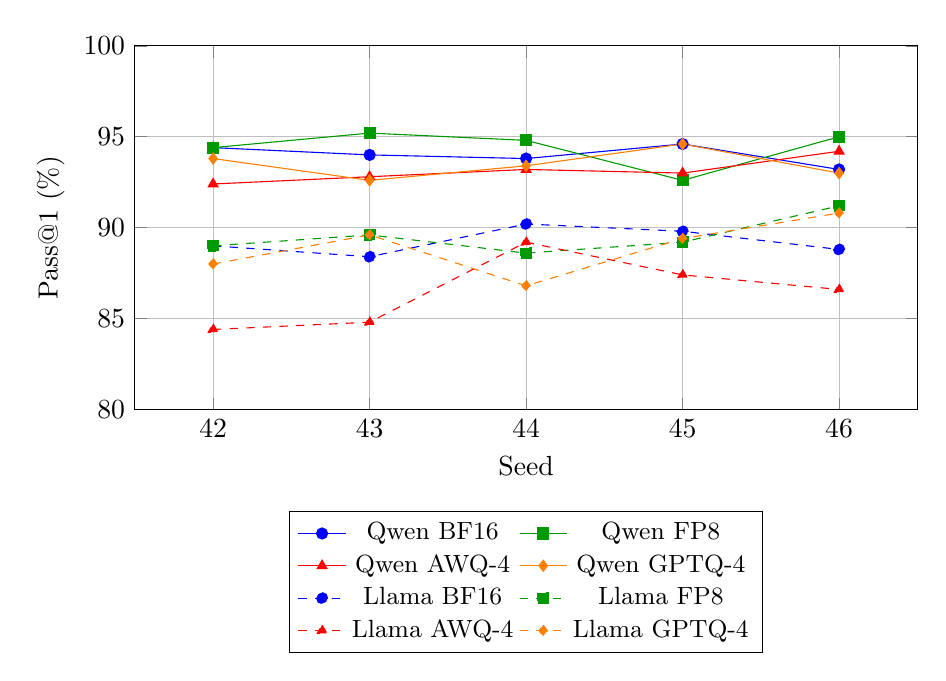
\begin{tikzpicture}
\begin{axis}[
    width=0.95\linewidth, height=6.2cm,
    xlabel={Seed},
    ylabel={Pass@1 (\%)},
    xmin=41.5, xmax=46.5,
    ymin=80, ymax=100,
    xtick={42,43,44,45,46},
    legend columns=2,
    legend style={font=\small, at={(0.5,-0.28)}, anchor=north},
    grid=major,
]
\addplot[blue, mark=*] coordinates {(42,94.4)(43,94.0)(44,93.8)(45,94.6)(46,93.2)};
\addplot[green!60!black, mark=square*] coordinates {(42,94.4)(43,95.2)(44,94.8)(45,92.6)(46,95.0)};
\addplot[red, mark=triangle*] coordinates {(42,92.4)(43,92.8)(44,93.2)(45,93.0)(46,94.2)};
\addplot[orange, mark=diamond*] coordinates {(42,93.8)(43,92.6)(44,93.4)(45,94.6)(46,93.0)};
\addplot[blue, dashed, mark=*] coordinates {(42,89.0)(43,88.4)(44,90.2)(45,89.8)(46,88.8)};
\addplot[green!60!black, dashed, mark=square*] coordinates {(42,89.0)(43,89.6)(44,88.6)(45,89.2)(46,91.2)};
\addplot[red, dashed, mark=triangle*] coordinates {(42,84.4)(43,84.8)(44,89.2)(45,87.4)(46,86.6)};
\addplot[orange, dashed, mark=diamond*] coordinates {(42,88.0)(43,89.6)(44,86.8)(45,89.4)(46,90.8)};
\legend{Qwen BF16, Qwen FP8, Qwen AWQ-4, Qwen GPTQ-4, Llama BF16, Llama FP8, Llama AWQ-4, Llama GPTQ-4}
\end{axis}
\end{tikzpicture}
\caption{MATH-500 pass@1 by seed. Solid: Qwen-7B. Dashed: Llama-8B. The tested Llama AWQ-4 checkpoint shows the largest MATH-500 pass@1 drop among the evaluated Llama cells.}
\label{fig:seed}
\end{figure}

\FloatBarrier
\subsection{Difficulty levels}
A per-level breakdown needs each row's MATH-500 \texttt{level}. The compact JSON stores items in the campaign pipeline order, which differs from the public release order: a positional join matches the public gold in only 118 of 11{,}382 integer-gold rows (counted over the $20{,}000$ MATH-500 completions: the $11{,}382$ correct completions whose public-order gold answer is an integer, of which $118$ have an extracted prediction equal to it). We therefore join on the exact question text in the stored campaign prompts; all 500 pipeline rows match distinct dataset items in both families.
Table~\ref{tab:levels} reports seed-averaged pass@1 by level. A post hoc linear trend of the AWQ-minus-BF16 item difference on level is $-1.25$ $[-2.36,-0.15]$\,pp per level for Llama AWQ-4 and $-0.15$ $[-0.96,+0.63]$ for Qwen AWQ-4; it assumes linearity in the level, is not multiplicity-adjusted, and the Llama interval nearly reaches zero.

\begin{table}[!htbp]
\centering
\caption{MATH-500 seed-averaged pass@1 (\%) by difficulty level, joined to the public dataset by exact question text. $n$: items per level. Last rows: Llama AWQ-4 (community upload) and Llama self-AWQ (our own quantization, Section~\ref{sec:res1}) minus BF16, paired difference (pp) with an item-level 95\% CI ($B=10{,}000$). Per-level intervals are exploratory.}
\label{tab:levels}
\small
\resizebox{\linewidth}{!}{%
\begin{tabular}{lccccc}
\toprule
\textbf{Cell} & \textbf{L1} & \textbf{L2} & \textbf{L3} & \textbf{L4} & \textbf{L5} \\
 & $n{=}43$ & $n{=}90$ & $n{=}105$ & $n{=}128$ & $n{=}134$ \\
\midrule
Qwen BF16 & 98.1 & 98.9 & 97.9 & 93.6 & 86.7 \\
Qwen FP8 & 98.1 & 98.2 & 98.1 & 94.5 & 87.6 \\
Qwen AWQ-4 & 97.2 & 97.6 & 97.5 & 93.9 & 84.6 \\
Qwen GPTQ-4 & 97.2 & 97.8 & 98.1 & 94.1 & 85.2 \\
\midrule
Llama BF16 & 95.3 & 94.7 & 95.0 & 90.5 & 77.9 \\
Llama FP8 & 95.3 & 96.7 & 94.3 & 90.0 & 78.7 \\
Llama AWQ-4 & 94.0 & 95.1 & 92.6 & 86.7 & 73.3 \\
Llama GPTQ-4 & 95.8 & 95.8 & 95.4 & 88.6 & 77.3 \\
Llama self-AWQ (E1) & 95.3 & 94.0 & 94.3 & 87.3 & 75.7 \\
\midrule
Llama AWQ-4 $-$ BF16 & $-1.40$ & $+0.44$ & $-2.48$ & $-3.75$ & $-4.63$ \\
 95\% CI & [$-5.58$, $+1.40$] & [$-2.44$, $+3.33$] & [$-4.95$, $-0.19$] & [$-6.41$, $-1.09$] & [$-8.06$, $-1.34$] \\
Llama self-AWQ $-$ BF16 & $+0.00$ & $-0.67$ & $-0.76$ & $-3.13$ & $-2.24$ \\
 95\% CI & [$-1.40$, $+1.40$] & [$-2.89$, $+1.56$] & [$-2.48$, $+0.95$] & [$-6.09$, $-0.16$] & [$-5.52$, $+0.90$] \\
\bottomrule
\end{tabular}%
}
\end{table}

\subsection{Item-level descriptive checks}
CPU-only reanalysis of the released compact JSON (\path{results/reports/item_level_descriptive_report.md}) is descriptive, not causal. MATH-500 has no item that is BF16-correct and quantized-wrong on all five seeds for any tested format. Incorrect MATH traces are longer than correct traces in every cell (for example, Qwen BF16 mean tokens $3{,}256$ when correct vs.\ $15{,}843$ when incorrect). GPQA-Diamond Qwen AWQ flips remain distributed (75 of 198 items flip on at least one seed; 0 items flip on all three seeds). These counts do not identify a small set of items that would explain the GPQA contrast.

\FloatBarrier
\section{Truncation, loops and the length signal}
\label{sec:pathology}
\paragraph{Pathology.}
A row is a \emph{loop} if the longest consecutive identical-word run is $\ge 20$ (Unicode word tokens, case-folded). The launcher sets both \texttt{max\_model\_len} and \texttt{max\_new\_tokens} to $32{,}768$. In vLLM the first bound is prompt plus output, so the effective output cap is $32{,}768$ minus that item's prompt length. Compact JSON has no \texttt{finish\_reason}. Tokenizing the stored campaign prompts with the frozen-runtime tokenizers (transformers~4.47.1) gives $29$--$811$ tokens (Qwen) and $27$--$776$ (Llama); the AWQ-4 prompts lack the two-token \texttt{<think>\textbackslash n} suffix and are shorter ($27$--$809$ and $25$--$774$). The effective cap therefore lies between $31{,}957$ and $32{,}743$ tokens. Re-tokenizing the stored completions with those tokenizers reproduces every stored \texttt{completion\_tokens} value ($56{,}408$ of $56{,}408$ completions); newer tokenizer releases do not (the Llama counts differ by about $220$ tokens per completion), so the prompt-length and cap analyses must run in the frozen environment (\path{scripts/analysis/audit_checks.py}). We therefore report \emph{near-cap} rows ($\ge 32{,}500$ tokens) as the truncation proxy. Because the stored prompts give each row its own cap, we also count \emph{cap-band} rows whose completion lies within 16 tokens of that per-item cap (Section~\ref{sec:pathology}). The tolerance is wider than necessary: with the frozen tokenizers $147$ of the $155$ cap-band rows are exactly at the cap and $154$ are within two tokens. The \texttt{boxed} flag is a string search for \texttt{\textbackslash boxed}, which is separate from extractive match.

Across 88 runs the validator records \textbf{25} repetition-flagged completions ($0.044\%$ of 56{,}408). The observed maximum completion length is $32{,}737$. Loops occur in BF16 as well as quantized cells (Llama MATH: 3/3/3/2 for BF16/FP8/AWQ/GPTQ). Three completions exceed 10{,}000 identical consecutive words. Near-cap completions ($\ge 32{,}500$ tokens) total 209; on MATH-500, Qwen AWQ-4/GPTQ-4 have 25 and 24 versus BF16's 14.

Near-cap rows are very likely truncations. Of the 140 MATH-500 near-cap rows, 121 lie between $32{,}600$ and $32{,}739$ tokens, the band where $32{,}768$ minus a typical prompt falls. Of the 57 GSM8K near-cap rows, 55 lie in that band. Only 24 MATH-500 rows and no GSM8K rows fall between the lowest possible cap ($31{,}957$) and $32{,}500$. The stored campaign prompts give each row its own cap. Cap-band rows number 155 on MATH-500 (Qwen 14 / 16 / 27 / 29 and Llama 20 / 11 / 15 / 23 for BF16 / FP8 / AWQ-4 / GPTQ-4). Of the 140 near-cap rows, 139 are in the cap band, so the two heuristics agree closely; the cap band flags 16 further suspected truncations of long-prompt items. Neither heuristic is a native stop-reason label, and near-cap rows are an upper bound on truncations: two near-cap rows that we checked individually (Qwen FP8 seed 44, item 417; Qwen GPTQ-4 seed 43, item 426) ended on their own with a boxed answer within 10 and 48 tokens of the cap, not by hitting it. Cap-band rows concentrate at difficulty levels 4 and 5 (129 of 155). On MATH-500, 120 of 134 unboxed rows are near-cap. A missing box on MATH is usually a long trace. It is not the 4-bit accuracy gap: unboxed rows that are still scored correct are rare (at most two per seed file), and boxed rates are $98.96$--$99.68\%$. GSM8K is similar (52 of 66 unboxed rows are near-cap; boxed rates $99.70$--$99.87\%$). GPQA is different: $4{,}746$ of $4{,}752$ rows are unboxed, and only 12 are near-cap. GPQA extractive match is not a boxed-answer grade, and the long-tail proxy does not explain it. Native stop reasons were not logged, but vLLM stops generation at $32{,}768$ minus the prompt length, and with the frozen tokenizers $147$ of the $155$ MATH-500 cap-band rows (and all $57$ near-cap GSM8K rows) have exactly that completion length; $7$ more lie within two tokens of it.

\begin{table}[!htbp]
\centering
\caption{Does a shorter completion predict a correct one (MATH-500, 5 seeds)? Pooled AUROC uses all 2{,}500 completions of a cell. Item-stratified AUROC uses only correct-versus-incorrect pairs within the same item, which removes item difficulty; its quantized-minus-BF16 difference uses shared item resamples. Item-level 95\% CIs. The last column counts items with at least one correct and one incorrect completion. Exploratory; from \texttt{scripts/analysis/trace\_failure\_analysis.py}.}
\label{tab:auroc}
\footnotesize
\setlength{\tabcolsep}{3pt}
\begin{tabular}{lcccc}
\toprule
\textbf{Cell} & \textbf{Pooled AUROC} & \textbf{Stratified AUROC} & \textbf{Stratified $-$ BF16} & \textbf{Items} \\
\midrule
Qwen BF16 & $0.936$ $[0.91,0.96]$ & $0.737$ $[0.63,0.84]$ & --- & 48 \\
Qwen FP8 & $0.927$ $[0.89,0.96]$ & $0.714$ $[0.62,0.81]$ & $-0.023$ $[-0.14,+0.09]$ & 48 \\
Qwen AWQ-4 & $0.925$ $[0.90,0.95]$ & $0.697$ $[0.60,0.78]$ & $-0.040$ $[-0.17,+0.08]$ & 59 \\
Qwen GPTQ-4 & $0.930$ $[0.90,0.96]$ & $0.763$ $[0.68,0.84]$ & $+0.027$ $[-0.10,+0.16]$ & 56 \\
\midrule
Llama BF16 & $0.875$ $[0.84,0.91]$ & $0.675$ $[0.61,0.74]$ & --- & 107 \\
Llama FP8 & $0.871$ $[0.82,0.91]$ & $0.664$ $[0.59,0.73]$ & $-0.011$ $[-0.10,+0.07]$ & 91 \\
Llama AWQ-4 & $0.830$ $[0.79,0.87]$ & $0.624$ $[0.56,0.68]$ & $-0.051$ $[-0.13,+0.03]$ & 134 \\
Llama GPTQ-4 & $0.901$ $[0.87,0.93]$ & $0.717$ $[0.65,0.78]$ & $+0.042$ $[-0.04,+0.12]$ & 110 \\
\bottomrule
\end{tabular}
\end{table}

\FloatBarrier
\section{Length detail}
\paragraph{Spread across seeds.} Completion length varies widely across seeds for the same item. For campaign BF16 the mean within-item standard deviation is $1{,}357$ tokens (Qwen) and $1{,}923$ (Llama), about $34\%$ and $41\%$ of the mean length (median item $587$ and $861$ tokens), so one run of one item says little about that item's length (Table~\ref{tab:lenvar}). The differences between formats are of the same size as the difference between two sets of unmodified BF16 seeds: five new Qwen BF16 seeds differ from the campaign seeds by $+186$ $[+12,+366]$ tokens, against $+247$ $[+70,+431]$ for AWQ-4 and $+344$ $[+162,+536]$ for GPTQ-4. We therefore do not read any format difference in this quantity as an effect of quantization on length stability, and the second BF16 row is the reference against which it should be judged.

% generated by analysis/gen_lenvar.py -- do not edit by hand
\begin{table}[t]
\centering
\caption{Within-item spread of completion length across seeds on MATH-500: for each item the standard deviation (tokens) over the five seeds, averaged over the 500 items, with item-level 95\% intervals ($B=10{,}000$); the median item is in the third column. The last column is the paired item-level difference from the campaign BF16 seeds. The second BF16 row, five new seeds of the same unmodified model, shows how much this quantity moves with no modification at all.}
\label{tab:lenvar}
\small
\resizebox{\linewidth}{!}{%
\begin{tabular}{lccc}
\toprule
\textbf{Arm} & \vcell{\textbf{Mean SD}}{(tokens)} & \textbf{Median SD} & \vcell{\textbf{Mean SD}}{$-$ campaign BF16} \\
\midrule
\multicolumn{4}{l}{\emph{Qwen-7B}} \\
BF16, campaign seeds 42--46 & \vcell{$1357$}{$[1185,1538]$} & 587 & --- \\
BF16, held-out seeds 47--51 (placebo) & \vcell{$1544$}{$[1335,1768]$} & 611 & \vcell{$+186$}{$[+12,+366]$} \\
FP8 & \vcell{$1496$}{$[1307,1693]$} & 679 & \vcell{$+138$}{$[-18,+296]$} \\
AWQ-4 & \vcell{$1604$}{$[1394,1825]$} & 646 & \vcell{$+247$}{$[+70,+431]$} \\
GPTQ-4 & \vcell{$1701$}{$[1468,1934]$} & 665 & \vcell{$+344$}{$[+162,+536]$} \\
BF16 at \texttt{float16} & \vcell{$1421$}{$[1242,1611]$} & 704 & \vcell{$+63$}{$[-100,+228]$} \\
BF16 at $T=0.8$ & \vcell{$1514$}{$[1343,1696]$} & 754 & \vcell{$+156$}{$[+17,+294]$} \\
\midrule
\multicolumn{4}{l}{\emph{Llama-8B}} \\
BF16, campaign seeds 42--46 & \vcell{$1923$}{$[1714,2142]$} & 861 & --- \\
BF16, held-out seeds 47--51 (placebo) & \vcell{$1886$}{$[1681,2100]$} & 912 & \vcell{$-37$}{$[-240,+155]$} \\
FP8 & \vcell{$1771$}{$[1585,1964]$} & 872 & \vcell{$-152$}{$[-340,+34]$} \\
AWQ-4 & \vcell{$1918$}{$[1721,2120]$} & 902 & \vcell{$-6$}{$[-209,+197]$} \\
GPTQ-4 & \vcell{$2109$}{$[1881,2353]$} & 913 & \vcell{$+186$}{$[-20,+398]$} \\
BF16 at \texttt{float16} & \vcell{$1785$}{$[1594,1990]$} & 836 & \vcell{$-138$}{$[-316,+40]$} \\
BF16 at $T=0.8$ & \vcell{$1728$}{$[1560,1910]$} & 927 & \vcell{$-195$}{$[-378,-13]$} \\
Self-quantized AWQ-4 & \vcell{$2039$}{$[1827,2260]$} & 956 & \vcell{$+116$}{$[-60,+292]$} \\
\bottomrule
\end{tabular}%
}
\end{table}


\label{app:length}
\begin{sidewaystable}
\centering
\caption{MATH-500 length versus BF16, all five seeds. RoM: ratio of means. $\Delta$: mean paired per-item token difference with an item-level 95\% CI. $2\times 2$ cells are mean quantized$-$BF16 $\Delta$ with an item-level 95\% CI and pair count $n$. BF16-correct and quant-correct columns use the same item resamples on Both-OK $\cup$ BF16-only and Both-OK $\cup$ Quant-only.}
\label{tab:tokens}
\small
\begin{tabular}{lcccccccc}
\toprule
\textbf{Contrast} & \textbf{RoM} & \textbf{Mean $\Delta$ [95\% CI]} & \textbf{Both OK} & \textbf{BF16 only} & \textbf{Quant only} & \textbf{Both wrong} & \textbf{BF16-correct} & \textbf{Quant-correct} \\
\midrule
Qwen FP8     & $-0.1\%$ & \vcell{$-4$}{$[-142,+134]$} & \vcell{$+51$ ($n{=}2297$)}{$[-42,+145]$} & \vcell{$+5444$ ($n{=}53$)}{$[+2922,+8035]$} & \vcell{$-6940$ ($n{=}63$)}{$[-9479,-4345]$} & \vcell{$+264$ ($n{=}87$)}{$[-1126,+1685]$} & \vcell{$+172$}{$[+63,+291]$} & \vcell{$-136$}{$[-273,-3]$} \\
Qwen AWQ-4   & $+6.3\%$ & \vcell{$+254$}{$[+116,+398]$} & \vcell{$+166$ ($n{=}2272$)}{$[+80,+254]$} & \vcell{$+6915$ ($n{=}78$)}{$[+4534,+9345]$} & \vcell{$-6533$ ($n{=}56$)}{$[-8933,-4255]$} & \vcell{$+894$ ($n{=}94$)}{$[-620,+2420]$} & \vcell{$+390$}{$[+261,+531]$} & \vcell{$+5$}{$[-111,+114]$} \\
Qwen GPTQ-4  & $+6.9\%$ & \vcell{$+276$}{$[+121,+431]$} & \vcell{$+136$ ($n{=}2284$)}{$[+45,+239]$} & \vcell{$+6892$ ($n{=}66$)}{$[+4090,+9896]$} & \vcell{$-4910$ ($n{=}53$)}{$[-8180,-1715]$} & \vcell{$+1893$ ($n{=}97$)}{$[+204,+3388]$} & \vcell{$+326$}{$[+198,+464]$} & \vcell{$+22$}{$[-99,+151]$} \\
Llama FP8    & $-2.3\%$ & \vcell{$-106$}{$[-284,+65]$} & \vcell{$+38$ ($n{=}2121$)}{$[-74,+152]$} & \vcell{$+2629$ ($n{=}110$)}{$[+1098,+4265]$} & \vcell{$-4159$ ($n{=}117$)}{$[-6040,-2428]$} & \vcell{$-968$ ($n{=}152$)}{$[-2252,+198]$} & \vcell{$+166$}{$[+33,+302]$} & \vcell{$-182$}{$[-339,-35]$} \\
Llama AWQ-4  & $+1.7\%$ & \vcell{$+80$}{$[-109,+268]$} & \vcell{$+91$ ($n{=}2052$)}{$[-25,+210]$} & \vcell{$+3090$ ($n{=}179$)}{$[+1995,+4286]$} & \vcell{$-4477$ ($n{=}110$)}{$[-6503,-2588]$} & \vcell{$-305$ ($n{=}159$)}{$[-1520,+907]$} & \vcell{$+332$}{$[+182,+490]$} & \vcell{$-141$}{$[-303,+12]$} \\
Llama GPTQ-4 & $+3.9\%$ & \vcell{$+184$}{$[+12,+359]$} & \vcell{$+66$ ($n{=}2097$)}{$[-43,+181]$} & \vcell{$+5915$ ($n{=}134$)}{$[+4335,+7605]$} & \vcell{$-4327$ ($n{=}126$)}{$[-6138,-2561]$} & \vcell{$+521$ ($n{=}143$)}{$[-506,+1585]$} & \vcell{$+417$}{$[+261,+583]$} & \vcell{$-183$}{$[-335,-35]$} \\
\bottomrule
\end{tabular}
\end{sidewaystable}

\begin{table}[!htbp]
\centering
\caption{Item-level mismatch excess $D=\overline{\Delta}_{\mathrm{BF16-only}}-\overline{\Delta}_{\mathrm{Both-OK}}$ on MATH-500. Both stratum means are formed on the same item resamples ($B=10{,}000$; empty-stratum replicates skipped; none occurred). $D$ is a diagnostic of correctness-conditioned mismatch asymmetry, not a causal quantization-induced token increase.}
\label{tab:mismatch-excess}
\small
\begin{tabular}{lccc}
\toprule
\textbf{Contrast} & \textbf{Both-OK $\Delta$} & \textbf{BF16-only $\Delta$} & \textbf{Mismatch excess $D$ [95\% CI]} \\
\midrule
Qwen FP8     & $+51\ [-42,+145]$ & $+5444\ [+2922,+8035]$ & $+5394\ [+2853,+7992]$ \\
Qwen AWQ-4   & $+166\ [+80,+254]$ & $+6915\ [+4534,+9345]$ & $+6748\ [+4375,+9184]$ \\
Qwen GPTQ-4  & $+136\ [+45,+239]$ & $+6892\ [+4090,+9896]$ & $+6755\ [+3938,+9786]$ \\
Llama FP8    & $+38\ [-74,+152]$ & $+2629\ [+1098,+4265]$ & $+2591\ [+1047,+4244]$ \\
Llama AWQ-4  & $+91\ [-25,+210]$ & $+3090\ [+1995,+4286]$ & $+2999\ [+1898,+4187]$ \\
Llama GPTQ-4 & $+66\ [-43,+181]$ & $+5915\ [+4335,+7605]$ & $+5849\ [+4258,+7553]$ \\
\bottomrule
\end{tabular}
\end{table}

\begin{figure}[!htbp]
\centering
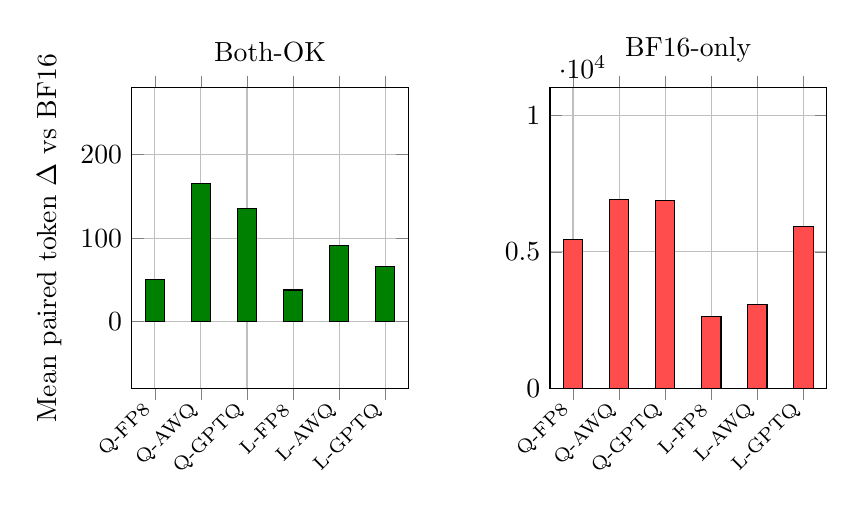
\begin{tikzpicture}
\begin{groupplot}[
    group style={
        group size=2 by 1,
        horizontal sep=1.8cm,
        ylabels at=edge left,
    },
    ybar,
    width=0.42\linewidth,
    height=5.4cm,
    symbolic x coords={Q-FP8, Q-AWQ, Q-GPTQ, L-FP8, L-AWQ, L-GPTQ},
    xtick=data,
    x tick label style={font=\scriptsize, rotate=45, anchor=east},
    grid=major,
]
\nextgroupplot[
    title={Both-OK},
    ylabel={Mean paired token $\Delta$ vs BF16},
    ymin=-80, ymax=280,
    bar width=7pt,
]
\addplot[fill=green!50!black] coordinates {(Q-FP8,51) (Q-AWQ,166) (Q-GPTQ,136) (L-FP8,38) (L-AWQ,91) (L-GPTQ,66)};
\nextgroupplot[title={BF16-only}, ymin=0, ymax=11000, bar width=7pt]
\addplot[fill=red!70] coordinates {(Q-FP8,5444) (Q-AWQ,6915) (Q-GPTQ,6892) (L-FP8,2629) (L-AWQ,3090) (L-GPTQ,5915)};
\end{groupplot}
\end{tikzpicture}
\caption{Paired token deltas by correctness, two panels so Both-OK is visible. Left: jointly-correct pairs (Qwen AWQ/GPTQ CIs exclude 0; FP8 and Llama CIs include 0; $n$ in Table~\ref{tab:tokens}). Right: BF16-correct / quantized-wrong pairs. Item-level 95\% CIs and $n$ are in Table~\ref{tab:tokens}.}
\label{fig:strata}
\end{figure}

\paragraph{Reflection markers.} A keyword count of self-checking phrases (``wait'', ``hmm'', ``alternatively'', check and verify phrases; Appendix Table~\ref{tab:reflection}) is higher in the longer 4-bit traces even among finished completions only (a comparison that conditions on finishing, so it does not describe the truncated traces): $+0.71$ $[+0.53,+0.89]$ markers per $1{,}000$ tokens for Qwen AWQ-4, $+0.91$ $[+0.68,+1.14]$ for Qwen GPTQ-4 and $+0.69$ $[+0.43,+0.94]$ for Llama GPTQ-4, whereas Llama AWQ-4, whose accuracy loss is the robust one, does not differ ($+0.05$ $[-0.20,+0.30]$). The pooled Qwen FP8 decrease ($-0.46$) disappears among finished completions ($-0.07$ $[-0.27,+0.14]$), so it reflected truncated traces. These are keyword counts, not an analysis of reasoning quality.

\begin{table}[!htbp]
\centering
\caption{Reflection-marker counts in the stored MATH-500 completions (regular expressions for ``wait'', ``hmm'', ``alternatively'', and check/verify phrases; keyword counts, not a semantic analysis). Columns: all markers per 1{,}000 tokens; the same for correct / incorrect finished (non-truncated) completions; and the quantized-minus-BF16 difference per 1{,}000 tokens, pooled over all completions and over finished (non-truncated) completions only, with item-level 95\% CIs ($B=10{,}000$). Exploratory; from \texttt{scripts/analysis/adaptive\_reflection\_rope.py}.}
\label{tab:reflection}
\footnotesize
\setlength{\tabcolsep}{2.5pt}
\begin{tabular}{lcccc}
\toprule
\textbf{Cell} & \textbf{All /1k} & \textbf{Correct / incorrect /1k} & \textbf{$-$ BF16, pooled} & \textbf{$-$ BF16, finished only} \\
\midrule
Qwen BF16 & 7.07 & 6.12 / 9.21 & --- & --- \\
Qwen FP8 & 6.61 & 6.04 / 9.57 & $-0.46$ $[-0.99,-0.04]$ & $-0.07$ $[-0.27,+0.14]$ \\
Qwen AWQ-4 & 7.76 & 6.91 / 9.51 & $+0.69$ $[+0.09,+1.33]$ & $+0.71$ $[+0.53,+0.89]$ \\
Qwen GPTQ-4 & 8.60 & 7.80 / 10.80 & $+1.52$ $[+0.53,+2.75]$ & $+0.91$ $[+0.68,+1.14]$ \\
\midrule
Llama BF16 & 9.43 & 8.84 / 10.92 & --- & --- \\
Llama FP8 & 9.44 & 8.84 / 11.30 & $+0.01$ $[-0.29,+0.30]$ & $+0.09$ $[-0.16,+0.33]$ \\
Llama AWQ-4 & 9.36 & 8.96 / 10.55 & $-0.06$ $[-0.38,+0.24]$ & $+0.05$ $[-0.20,+0.30]$ \\
Llama GPTQ-4 & 10.30 & 9.28 / 12.07 & $+0.88$ $[+0.43,+1.35]$ & $+0.69$ $[+0.43,+0.94]$ \\
\bottomrule
\end{tabular}
\end{table}

\FloatBarrier
\section{Secondary analyses: serving cost and gold-free abstention}
\label{app:secondary}
These two analyses use the same campaign records as the main text but answer different questions (what a serving measurement can and cannot rank, and how a second sample can replace a gold label). They are reported here in full; the main text gives only their headline numbers.

\paragraph{Cost.} Erol et al.~\cite{erol2025costofpass} define Cost-of-Pass as the expected monetary cost per correct solution; our aggregate proxies follow its form but are not its per-problem estimator.

\paragraph{Agreement and selective prediction.} Self-consistency~\cite{wang2022selfconsistency} aggregates samples by majority vote, and G-Pass@$k$~\cite{liu2025gpass} measures stability across samples; both are different estimands from ours. We use answer agreement as a gold-free abstention signal in the selective-classification framework of Geifman and El-Yaniv~\cite{geifman2017selective}, and compare it at matched coverage with a one-sample length rule.

\subsection{Cost estimands}
\label{sec:cost-def}
Measured serving yields output tokens per second (tok/s) and GPU-seconds per query on a prompt subset. We combine them with campaign accuracy in a hybrid Cost-of-Pass proxy,
\begin{equation}
\widetilde{C}_{\mathrm{pass}}^{\mathrm{hyb}} = \frac{(\text{GPU-sec/query})\times (\$1.50/3600)}{\mathrm{pass@1}},
\end{equation}
where $\$1.50$ per A100-hour is a pricing scenario that rescales costs without reranking them. Because subset GPU-seconds inherit the subset's trace lengths, we also report \emph{campaign-length seconds per correct answer}: the full-grid mean length divided by the measured tok/s (total tokens over total time) and by pass@1. To isolate the length draw we simulate $20{,}000$ random 20-prompt subsets, stratified four per MATH level, give each format one randomly chosen campaign seed, and hold tok/s fixed. Neither proxy is Erol et al.'s per-problem estimator.

\subsection{Serving stack and timing}
\label{sec:serving-timing}
After the accuracy campaign we timed all eight checkpoints on two MATH-500 subsets drawn from campaign items: \emph{Condition~A}, 20 prompts (four per level) decoded sequentially, and \emph{Condition~B}, 100 prompts (20 per level) in one \texttt{llm.generate} call with \texttt{max\_num\_seqs=8}. Each condition was repeated three times (five when the coefficient of variation exceeded $3\%$) after three discarded warmups. All repeats share one sampling seed, so their spread is wall-clock jitter at a fixed aggregate length, not length variance. Qwen and Llama ran on different two-GPU nodes without exclusive allocation, and formats ran sequentially within a day. Appendix~\ref{sec:measured-serving} gives the full protocol.

\subsection{Serving cost: one subset is one length draw}
\label{sec:cost-results}
\paragraph{Small subsets reorder formats.} Table~\ref{tab:subsetsim} isolates the length draw. With measured tok/s held fixed, the format that is cheapest at campaign length is cheapest in only $58\%$ (Qwen, GPTQ-4) and $62\%$ (Llama, FP8) of random 20-prompt subsets, and the full four-format order is reproduced in only $40\%$ and $21\%$ of draws. A few very long traces dominate the mean length of a small subset, and GPU-seconds are output tokens divided by tok/s, so a long draw raises cost even when the kernel is faster.

\begin{table}[t]
\centering
\caption{Subset-draw simulation for Condition~A. Each of $20{,}000$ draws takes a random 20-prompt MATH-500 subset stratified four per difficulty level, assigns each format one randomly chosen campaign seed, and costs it as subset mean tokens $\div$ measured Condition~A tok/s $\div$ campaign pass@1. Columns: probability that each format is cheapest (bold: the campaign-length cheapest format of Table~\ref{tab:length-cost}) and probability that the full four-format order equals the campaign-length order. Only the length draw varies; tok/s is held fixed, so no timing or host uncertainty is included.}
\label{tab:subsetsim}
\small
\begin{tabular}{lccccc}
\toprule
 & \multicolumn{4}{c}{\textbf{P(cheapest)}} & \textbf{P(order} \\
\cmidrule(lr){2-5}
\textbf{Family} & BF16 & FP8 & AWQ-4 & GPTQ-4 & \textbf{= campaign)} \\
\midrule
Qwen-7B & 0.000 & 0.078 & 0.343 & \textbf{0.580} & 0.403 \\
Llama-8B & 0.243 & \textbf{0.616} & 0.104 & 0.037 & 0.206 \\
\bottomrule
\end{tabular}
\end{table}

\paragraph{Campaign-length costs are stable.} Substituting the campaign mean length for the subset length (Table~\ref{tab:length-cost}) makes Qwen GPTQ-4 cheapest on both conditions and Llama FP8 cheapest on both conditions. In an item bootstrap of campaign tokens and pass@1 with tok/s fixed, Llama FP8 ranks first on both conditions in all $10{,}000$ resamples, and Qwen GPTQ-4 in $99.9\%$ (Condition~A) and $97.55\%$ (Condition~B).

\begin{table}[t]
\centering
\caption{Campaign-length seconds per correct answer: full-grid mean MATH-500 tokens $\div$ measured tok/s $\div$ pass@1. Tok/s (the A and B columns) is total tokens over total time of the confirmation repeats and is held fixed; with the mean MATH-500 tokens and pass@1 of the campaign tables, the seconds can be recomputed from the printed values. Lower is cheaper. This is a sensitivity to subset length, not a replacement for Table~\ref{tab:serving-main}.}
\label{tab:length-cost}
\small
\begin{tabular}{llcccccc}
\toprule
\textbf{Model} & \textbf{Fmt} & \textbf{A tok/s} & \textbf{A sec.} & \textbf{A rank} & \textbf{B tok/s} & \textbf{B sec.} & \textbf{B rank} \\
\midrule
Qwen-7B & BF16 & 43.92 & 97.16 & 4 & 252.72 & 16.89 & 4 \\
Qwen-7B & FP8 & 62.50 & 67.93 & 3 & 432.54 & 9.82 & 2 \\
Qwen-7B & AWQ-4 & 76.89 & 59.57 & 2 & 418.15 & 10.95 & 3 \\
Qwen-7B & GPTQ-4 & 82.67 & 55.48 & 1 & 488.25 & 9.39 & 1 \\
Llama-8B & BF16 & 72.33 & 72.14 & 2 & 366.98 & 14.22 & 3 \\
Llama-8B & FP8 & 78.68 & 64.61 & 1 & 481.42 & 10.56 & 1 \\
Llama-8B & AWQ-4 & 70.11 & 78.12 & 3 & 391.11 & 14.00 & 2 \\
Llama-8B & GPTQ-4 & 63.49 & 85.74 & 4 & 366.16 & 14.87 & 4 \\
\bottomrule
\end{tabular}
\end{table}

\paragraph{The measured subset shows the problem.} On the measured 20-prompt Condition~A subset, the hybrid cost ranks Llama BF16 cheapest ($\$0.0310$ against about $\$0.043$ for FP8 and AWQ-4; Appendix Table~\ref{tab:serving-main}), the opposite of the campaign-length order. Measured subset lengths exceed the campaign means on the same prompts for FP8 in all four family-by-condition groups (ratios $1.07$--$1.49$; Appendix Table~\ref{tab:subsetlen}). We cannot attribute this excess. A tail draw is possible but not established, and the timer differs from the campaign in scheduling, seed and one extra beginning-of-sequence token per request (Appendix~\ref{sec:serving-results}). Timing repeats that share a sampling seed cannot expose any of this. Throughput itself carries a caveat: Qwen BF16 decodes anomalously slowly on its node ($43.92$ tok/s against $72.34$ for the larger Llama-8B on Condition~A, and $205.41$ against $362.01$ in a fixed-length microbenchmark), so the Qwen savings are relative to a baseline of unknown bias. We therefore report measured dollars as a property of these subsets and nodes, not as a deployment ranking.

\subsection{Gold-free agreement}
\label{sec:modal-def}
MATH-500 answers are clustered into mathematical-equivalence classes with the campaign evaluator (LightEval~0.8.0 with math-verify). The \emph{$k$-sample unanimity} rule serves an item when all $k$ answers fall in one class; coverage and selective risk~\cite{geifman2017selective} are averaged over all $\binom{5}{k}$ seed subsets, and the token cost is $k$ times the mean completion length. Modal rules serve when a unique modal class has at least $m$ of five votes. The comparator is a one-sample \emph{length rule} that, for each seed, serves the shortest traces up to the coverage of the agreement rule. Gold answers are used only to score served predictions.

\subsection{Gold-free abstention: the second sample does most of the work}
\label{sec:modal}
Unanimity of two samples serves $82.1$--$92.7\%$ of MATH-500 items at $0.69$--$2.36\%$ selective risk (Table~\ref{tab:agree}, Figure~\ref{fig:agree}). A one-sample length rule at the same coverage has $2.16$--$5.84\%$ risk, $2.2$--$3.1$ times higher, at half the tokens. Three samples reach $0.18$--$1.07\%$, and five-sample unanimity at most $0.27\%$ at $70.2$--$88.8\%$ coverage; zero observed errors in a cell still has a Wilson 95\% upper bound of $0.82$--$1.08\%$. Every $k$ beats the matched length rule in every cell, and most of the gain arrives with the second sample. An adaptive rule---draw two samples and serve if they agree; otherwise draw three more and serve a unique mode with at least three of five votes---reaches the operating point of the fixed $\ge3/5$ rule (coverage $0.2$--$0.6$\,pp higher, risk $0.05$--$0.41$\,pp higher) at $37$--$46\%$ fewer tokens (Appendix Table~\ref{tab:adaptive}).

\begin{table}[t]
\centering
\caption{Gold-free abstention on MATH-500 by $k$-sample unanimity. Cov.: coverage; Risk: selective risk among served items; Len.: risk of a one-sample shortest-trace rule at the same coverage. Percentages, averaged over all $\binom{5}{k}$ seed subsets (length rule: over five seeds). Token cost per item is $k$ times the mean completion length: about $8.0$--$8.6$k (Qwen) and $9.1$--$9.7$k (Llama) tokens at $k=2$, and $20.0$--$21.4$k and $22.8$--$24.2$k at $k=5$. The $k=4$ column and the modal rules are in Appendix~\ref{app:modal}.}
\label{tab:agree}
\small
\begin{tabular}{llccccccccc}
\toprule
 & & \multicolumn{3}{c}{$k=2$} & \multicolumn{3}{c}{$k=3$} & \multicolumn{3}{c}{$k=5$} \\
\cmidrule(lr){3-5}\cmidrule(lr){6-8}\cmidrule(lr){9-11}
\textbf{Model} & \textbf{Fmt} & Cov. & Risk & Len. & Cov. & Risk & Len. & Cov. & Risk & Len. \\
\midrule
Qwen-7B & BF16 & 92.5 & 0.89 & 2.20 & 90.7 & 0.44 & 1.94 & 88.4 & 0.23 & 1.67 \\
Qwen-7B & FP8 & 92.7 & 0.69 & 2.16 & 90.7 & 0.18 & 1.94 & 88.8 & 0.00 & 1.71 \\
Qwen-7B & AWQ-4 & 91.2 & 1.05 & 2.54 & 88.8 & 0.43 & 2.34 & 86.4 & 0.23 & 1.99 \\
Qwen-7B & GPTQ-4 & 91.6 & 0.87 & 2.31 & 89.3 & 0.29 & 1.92 & 86.6 & 0.00 & 1.62 \\
\midrule
Llama-8B & BF16 & 85.8 & 1.86 & 4.06 & 81.5 & 0.71 & 3.34 & 76.2 & 0.26 & 2.83 \\
Llama-8B & FP8 & 86.9 & 1.91 & 4.47 & 82.9 & 0.63 & 3.82 & 78.2 & 0.00 & 3.17 \\
Llama-8B & AWQ-4 & 82.1 & 2.36 & 5.84 & 76.8 & 1.07 & 4.90 & 70.2 & 0.00 & 4.56 \\
Llama-8B & GPTQ-4 & 85.1 & 1.76 & 4.08 & 80.5 & 0.62 & 3.03 & 75.4 & 0.27 & 2.55 \\
\bottomrule
\end{tabular}
\end{table}

\begin{figure}[t]
\centering
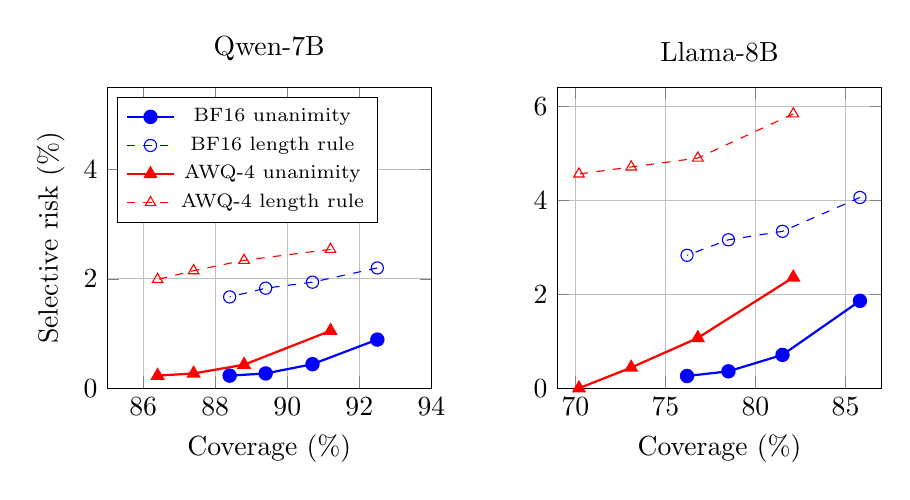
\begin{tikzpicture}
\begin{groupplot}[
    group style={group size=2 by 1, horizontal sep=1.6cm, ylabels at=edge left},
    width=0.47\linewidth, height=5.4cm,
    xlabel={Coverage (\%)},
    ylabel={Selective risk (\%)},
    grid=major,
    legend style={font=\scriptsize, at={(0.03,0.97)}, anchor=north west},
]
\nextgroupplot[title={Qwen-7B}, xmin=85, xmax=94, ymin=0, ymax=5.5]
\addplot[blue, thick, mark=*, mark size=2.2pt] coordinates {(92.5,0.89) (90.7,0.44) (89.4,0.27) (88.4,0.23)};
\addplot[blue, dashed, mark=o, mark size=2.2pt, mark options={solid}] coordinates {(92.5,2.2) (90.7,1.94) (89.4,1.83) (88.4,1.67)};
\addplot[red, thick, mark=triangle*, mark size=2.2pt] coordinates {(91.2,1.05) (88.8,0.43) (87.4,0.27) (86.4,0.23)};
\addplot[red, dashed, mark=triangle, mark size=2.2pt, mark options={solid}] coordinates {(91.2,2.54) (88.8,2.34) (87.4,2.15) (86.4,1.99)};
\legend{BF16 unanimity, BF16 length rule, AWQ-4 unanimity, AWQ-4 length rule}
\nextgroupplot[title={Llama-8B}, xmin=69, xmax=87, ymin=0, ymax=6.4]
\addplot[blue, thick, mark=*, mark size=2.2pt] coordinates {(85.8,1.86) (81.5,0.71) (78.5,0.36) (76.2,0.26)};
\addplot[blue, dashed, mark=o, mark size=2.2pt, mark options={solid}] coordinates {(85.8,4.06) (81.5,3.34) (78.5,3.16) (76.2,2.83)};
\addplot[red, thick, mark=triangle*, mark size=2.2pt] coordinates {(82.1,2.36) (76.8,1.07) (73.1,0.44) (70.2,0)};
\addplot[red, dashed, mark=triangle, mark size=2.2pt, mark options={solid}] coordinates {(82.1,5.84) (76.8,4.9) (73.1,4.71) (70.2,4.56)};
\end{groupplot}
\end{tikzpicture}
\caption{Selective risk against coverage on MATH-500 for $k$-sample unanimity (solid; from left to right $k=5,4,3,2$) and for a one-sample shortest-trace rule at the same coverage (dashed). At every coverage, agreement has the lower risk; the step from one to two samples gives most of the reduction. BF16 and AWQ-4 are shown; all eight cells are in Table~\ref{tab:agree} and Appendix Table~\ref{tab:kcurve}.}
\label{fig:agree}
\end{figure}

Agreement also registers the robust accuracy loss: Llama AWQ-4 serves $70.2\%$ of items at 5/5 unanimity against $76.2\%$ for BF16 ($-6.0$\,pp $[-9.4,-2.6]$; Appendix Table~\ref{tab:modal-paired}). The length rule is weak mainly because length separates easy items from hard ones: the pooled length AUROC of $0.83$--$0.94$ falls to $0.62$--$0.76$ within items, and no quantized checkpoint differs detectably from BF16 on the within-item AUROC (Appendix Table~\ref{tab:auroc}). Token-level confidence was not stored, so a stronger single-sample comparator remains untested.


\section{Measured serving}
\label{app:serving}
\subsection{Protocol}
\label{sec:measured-serving}
After the 56k accuracy campaign we timed the same eight checkpoints on A100-80GB under vLLM~0.7.0 eager. Primary numbers are the controlled confirmation (protocol: \path{docs/MEASURED_SERVING_CONFIRMATION_PROTOCOL.md}; raw JSON under \path{results/measured_serving_confirmation/raw/}). Condition~A is 20 sequential MATH-500 prompts (4 per difficulty level; both subsets are drawn from the campaign items, and the released subset files list each prompt with its \texttt{campaign\_index}). Condition~B is 100 prompts (20 per level) in one \texttt{llm.generate} call with \texttt{max\_num\_seqs=8}. The two conditions differ in both the prompt subset and the serving regime, so a ranking change between them is a property of the whole condition. With \texttt{max\_num\_seqs=8}, Condition~B elapsed time runs until the last trace finishes. One or two long traces can decode alone after the batch drains. The raw JSON stores aggregate tokens and elapsed time, not time spent below a full batch of 8, so that tail share is not reported. A secondary microbenchmark forces 10 prompts to 512 tokens (\texttt{ignore\_eos}). The timer passes the stored prompt strings to vLLM, which tokenizes them with a second beginning-of-sequence token: every request has one more input token than the frozen-tokenizer recount of the stored prompt (for example 1{,}986 versus 1{,}966 input tokens for the 20 Qwen Condition~A prompts, in all four formats; the same holds in every cell and condition). This is not a difference from the campaign: rerunning the frozen campaign code shows the engine's prompt length equal to the recount plus one on all 500 MATH-500 rows (Appendix~\ref{app:followup}), so the campaign engine received the same doubled token. The AWQ-4 timer prompts still differ from their own accuracy-campaign prompts by the \texttt{<think>\textbackslash n} suffix that the AWQ-4 accuracy prompts lack.

Three warmup queries are discarded. $\Delta t_{\mathrm{steady}}$ is then the wall-clock from the first measured request to the return of the last measured response, bracketed by \texttt{torch.cuda.synchronize()}. Engine initialization is outside that interval. The first measured prefill and the straggler tail are inside it. Output tok/s $=(\sum \text{output tokens})/\Delta t_{\mathrm{steady}}$. GPU-sec/query $=\Delta t_{\mathrm{steady}}/N$ on one GPU. Sampling matches the campaign ($T=0.6$, top-$p=0.95$) with seed $20260816$. Repetitions share that seed, and the recorded aggregate output-token counts are identical across repeats (the generated sequences were not retained, so identity of the sequences is not verified). The tok/s spread is wall-clock jitter at a fixed aggregate length. It is not length variance. $R=3$, expanded to $R=5$ when the CV of the first three tok/s values exceeds $3\%$; as implemented, that CV uses the population standard deviation (Llama FP8 Condition~A sits at $2.995\%$ and keeps $R=3$; the sample-SD CV would be $3.67\%$ and would have triggered $R=5$), whereas the reported tok/s spreads are sample SDs. With three repeats a percentile interval has at most ten distinct means. We therefore report the sample mean, the sample SD, and the observed min--max, and we do not treat those intervals as a stable estimate of timing noise. Qwen-7B jobs ran on \texttt{ragpu003} and Llama-8B jobs on \texttt{ragpu004}; both are two-GPU nodes, and each SLURM job requested one GPU and 16 CPU cores without \texttt{--exclusive}. The raw records log NVIDIA driver 550.54.14 on both hosts. Within a family, all four formats share a host but ran sequentially on one day (Qwen: BF16 05:36, FP8 08:29, AWQ-4 11:09, GPTQ-4 12:38 UTC), so format is also confounded with time on a node that other jobs could share. Eager decode is bound by kernel-launch CPU time, so host load moves single-stream tok/s. Across families, host and architecture are confounded. Archived logs do not contain per-run clocks, power, or co-tenant load. Peak VRAM is \texttt{torch.cuda.max\_memory\_allocated} after the $0.75$ utilization preallocation.

\begin{equation}
\widetilde{C}_{\mathrm{pass}}^{\mathrm{hyb}} = \frac{(\text{GPU-sec/query})\times (\$1.50/3600)}{\mathrm{pass@1}},
\end{equation}
The numerator is subset GPU-seconds and the denominator is the frozen MATH-500 campaign pass@1. This ratio follows the Cost-of-Pass form and is not the per-problem estimator of Erol et al.~\cite{erol2025costofpass}. Because the repeats share a seed, the printed interval multiplies wall-clock jitter by a pass@1 bootstrap. It does not resample prompt lengths. A second estimator holds measured tok/s fixed and substitutes the campaign mean length: campaign tokens $\div$ tok/s $\div$ pass@1, with tok/s taken as total tokens over total time across the repeats (the aggregate that matches the reported GPU-s/q and hybrid dollars; it differs from the mean of per-repeat ratios only for Qwen FP8 Condition~B, which varied by $56\%$ across repeats, and in the third digit elsewhere). That estimator still uses a length-dependent tok/s, so it is a sensitivity, not a replacement measurement. The $\$1.50$/A100-hour rate is a pricing scenario. Because it is a single constant, it rescales GPU-seconds without changing any ranking.

\subsection{Measurements and forensics}
\label{sec:serving-results}
This section does not claim a deployment cost ranking. Its finding is a mechanism: a few very long traces dominate the mean length of a small subset, so one draw of reasoning lengths can reorder cells that campaign-length costs order differently (Table~\ref{tab:length-cost}). Table~\ref{tab:serving-main} is the supporting measurement; it separates tok/s from GPU-seconds per query. GPU-seconds equal output tokens divided by tok/s, so a long subset draw raises cost even when the kernel is faster. To size the effect we drew $20{,}000$ random 20-prompt subsets stratified four per MATH level, gave each format one randomly chosen campaign seed, and held the measured Condition~A tok/s fixed (Appendix Table~\ref{tab:subsetsim}). The campaign-length cheapest format is cheapest in only $58\%$ of draws for Qwen (GPTQ-4) and $62\%$ for Llama (FP8), and the full four-format order equals the campaign-length order in $40\%$ and $21\%$ of draws. This simulation varies only the length draw and carries no timing or host uncertainty; it is the evidence for the mechanism.

The largest case among the measured subsets is Llama FP8 on Condition~A. Within a repeat, output tokens equal tok/s times GPU-s/q; the three repeats each record $145{,}647/20=7{,}282.35$ tokens per query (the product of the printed means, $78.75\times 92.55$, gives $7{,}288$ only because a mean of ratios is not a ratio of means). The campaign mean on the same 20 prompts is $4{,}889$ tokens, and $4{,}550.8$ on the full grid, which is $2.3\%$ shorter than Llama BF16. Across the sixteen cell-by-condition comparisons of measured subset length with the campaign mean on the same prompts (Appendix Table~\ref{tab:subsetlen}) the ratio ranges from $0.88$ to $1.49$; Llama FP8 Condition~A is the maximum ($1.49$) and Qwen FP8 Condition~A is next ($1.35$). The latency percentiles of the $20$ sequential requests (p90 of $19{,}334$--$20{,}314$ and p95 of $26{,}489$--$27{,}135$ tokens at the measured tok/s) imply about three requests of roughly $18{,}000$ tokens or more, whereas the campaign reaches $15{,}000$ tokens in $5.7\%$ of Llama FP8 completions; under a beta-binomial count model, three or more such traces among $20$ prompts has probability of at most about $4\%$ ($10\%$ with a pooled rate). Resampling the five stored completions of those prompts exceeds $7{,}282$ in only $19$ of $20{,}000$ draws, but five completions per prompt truncate the tail and overstate the rarity. We cannot attribute this excess. FP8 has the highest measured-to-campaign ratio in all four groups ($1.35$ and $1.07$ for Qwen, $1.49$ and $1.09$ for Llama on Conditions A and B), the model files, quantization backend, prefix caching, chunked prefill and KV dtype are the same in both runs, and the campaign shows no elevated count of near-cap FP8 completions. What differs is single-stream versus batched scheduling and the seed (Section~\ref{sec:measured-serving}; the extra input token of the timer is also present in the campaign); the per-request lengths were not stored. A tail draw is possible but not established, and a single-BOS, multi-seed GPU rerun, which we have not run, would separate the explanations. Condition~A's ranking of Llama BF16 as cheapest ($\$0.0310$ vs.\ about $\$0.043$) is therefore reported as a measurement of that subset, not as a stable ranking. Llama GPTQ-4 Condition~B tok/s is $0.2\%$ below BF16 ($366.16$ vs.\ $366.98$) while hybrid cost is $+24.9\%$; the gap is mostly length.

The brackets in Table~\ref{tab:serving-main} are the minimum and maximum hybrid cost across timing repeats, with campaign pass@1 held fixed. They are not a 95\% interval. Repeats share seed $20260816$, so they do not include length variance. Qwen BF16 Condition~A tok/s runs only from $43.88$ to $43.96$. Qwen FP8 Condition~B runs from $350.68$ to $546.26$, and its dollar min--max is $\$0.0030$--$\$0.0047$. Qwen FP8 Condition~B tok/s of $449.79$ in Table~\ref{tab:serving-main} is the mean of five ratios. Mean GPU-s/q is $8.64$, and total tokens over total time is $432.5$ tok/s, which is what the reported GPU-s/q and hybrid dollars imply. The campaign-length seconds below use total tokens over total time for every cell. Appendix Table~\ref{tab:fp8-reps} lists the five repeats. Llama FP8 and AWQ-4 Condition~A means both round to $\$0.0431$. Their repeat ranges do not: $\$0.0421$--$\$0.0449$ and $\$0.0423$--$\$0.0463$.

Table~\ref{tab:length-cost} substitutes campaign mean tokens for the subset length and keeps the measured tok/s (total tokens over total time). Under that sensitivity, Qwen GPTQ-4 is cheapest on both conditions, so the AWQ/GPTQ reversal between A and B disappears. Llama FP8 is cheapest on both conditions and on mean tokens divided by pass@1. An item bootstrap of campaign tokens and pass@1, with tok/s held fixed ($B=10{,}000$), gives Llama FP8 rank~1 on both campaign-length costs in all $10{,}000$ draws. Qwen GPTQ-4 is rank~1 on Condition~A in $99.9\%$ of draws and on Condition~B in $97.55\%$, with FP8 taking $2.45\%$; with the mean of per-repeat ratios, which overstates Qwen FP8's tok/s, the Condition~B split would be $59.6\%$ against $40.4\%$. These resamples hold tok/s fixed, so they carry no timing uncertainty, and Qwen FP8's Condition~B tok/s varied by $56\%$ across repeats (Appendix Table~\ref{tab:fp8-reps}). Measured tok/s still depends on the subset's length, so Table~\ref{tab:length-cost} is not a final serving measurement. Figure~\ref{fig:condB-scatter} plots the Condition~B campaign-length seconds, not the subset dollars.

Qwen BF16 decodes at $43.92$ tok/s on Condition~A and $205.41$ tok/s in the fixed-512 microbenchmark. Llama BF16, on the other host, reaches $72.34$ and $362.01$. The fixed-length gap remains, so it is not the Condition~A length draw. The microbenchmark controls output length but still includes prefill, scheduling, and host overhead, so it does not isolate pure kernel decode speed. The Qwen BF16 baseline looks anomalous. Qwen-7B is the smaller model, yet it decodes about $40\%$ slower than Llama-8B BF16. In the fixed-length microbenchmark FP8 speeds up Qwen by $2.13\times$ ($437.19/205.41$) but Llama by only $1.08\times$ ($392.05/362.01$), even though both use the same Marlin W8A16 kernel. Every Qwen Condition~B saving in Table~\ref{tab:serving-main} ($-36.0\%$ to $-45.9\%$) is relative to that baseline, which ran first on \texttt{ragpu003}. The Qwen FP8 Condition~B repeats stepped up in run order ($350.9$, $350.7$, $455.9$, $545.2$, $546.3$ tok/s), which is consistent with changing runtime conditions, although host load is not identified as the cause. We therefore treat the Qwen savings as potentially confounded estimates whose bias direction is unknown; a controlled, interleaved same-node rerun would be needed to confirm them. Clocks were not logged. For AWQ-4 the backend is explained in Section~\ref{sec:formats}. AWQ-Marlin is typically faster on A100 for compatible checkpoints, so every AWQ throughput number reflects the backend available to these artifacts as well as the format. That can contribute to Llama AWQ-4 decoding more slowly than BF16 on Condition~A ($70.20$ vs.\ $72.34$ tok/s). GPTQ-4 timing used \texttt{float16} while GPTQ-4 pass@1 used \texttt{bfloat16}, so the hybrid ratio joins two configurations. For AWQ-4 the timer also passes stored prompts that already include the \texttt{<think>} suffix, which the accuracy-campaign AWQ-4 prompts omit, so the AWQ-4 hybrid ratio likewise joins two configurations. These FP8 numbers are A100 Marlin W8A16, not Hopper W8A8. Peak allocated VRAM is $53.9$--$56.1$\,GB, the $0.75$ engine pool. Condition~A latency is in Appendix Table~\ref{tab:serving-single}.

Condition~A latency detail (Table~\ref{tab:serving-single}) is sequential decode of a balanced 20-prompt MATH-500 subset. Median latency is the mean of per-run medians. $R=3$ except Llama AWQ-4 ($R=5$; CV-triggered). Fixed-token microbenchmark (Table~\ref{tab:serving-micro}): 10 prompts $\times$ 512 tokens, $T=0.0$, \texttt{ignore\_eos}. Table~\ref{tab:fp8-reps} lists all five Qwen FP8 Condition~B repeats. Table~\ref{tab:economics} reports mean tokens divided by pass@1. It is not measured wall-clock.

\begin{sidewaystable}
\centering
\caption{Hybrid cost on the controlled confirmation. Condition~A: 20 sequential prompts. Condition~B: 100-prompt \texttt{llm.generate}, \texttt{max\_num\_seqs=8}. Tok/s is mean$\pm$ sample SD. Brackets are the minimum and maximum hybrid cost across timing repeats, with campaign pass@1 held fixed. They are not a 95\% interval. The B $\Delta$\% column is the point estimate only. Qwen: \texttt{ragpu003}. Llama: \texttt{ragpu004}. GPTQ dollars join \texttt{float16} timing with \texttt{bfloat16} pass@1.}
\label{tab:serving-main}
\small
\begin{tabular}{llccccccc}
\toprule
\textbf{Model} & \textbf{Fmt} & \textbf{A tok/s} & \textbf{A GPU-s/q} & \textbf{A $\widetilde{C}$ [min, max]} & \textbf{B tok/s} & \textbf{B GPU-s/q} & \textbf{B $\widetilde{C}$ [min, max]} & \textbf{B $\Delta$\%} \\
\midrule
Qwen-7B & BF16   & $43.92\pm 0.04$ & 102.51 & \$0.0454 [0.0454, 0.0455] & $252.72\pm 0.56$ & 13.44 & \$0.0060 [0.0059, 0.0060] & anchor \\
Qwen-7B & FP8    & $62.50\pm 0.08$ & 84.60 & \$0.0373 [0.0373, 0.0374] & $449.79\pm 97.53$ & 8.64 & \$0.0038 [0.0030, 0.0047] & $-36.0$ \\
Qwen-7B & AWQ-4  & $76.89\pm 0.70$ & 48.04 & \$0.0215 [0.0213, 0.0217] & $418.15\pm 2.03$ & 7.82 & \$0.0035 [0.0035, 0.0035] & $-41.3$ \\
Qwen-7B & GPTQ-4 & $82.67\pm 0.69$ & 54.39 & \$0.0242 [0.0241, 0.0245] & $488.26\pm 0.64$ & 7.23 & \$0.0032 [0.0032, 0.0032] & $-45.9$ \\
\midrule
Llama-8B & BF16   & $72.34\pm 0.27$ & 66.43 & \$0.0310 [0.0309, 0.0311] & $366.98\pm 1.90$ & 10.13 & \$0.0047 [0.0047, 0.0048] & anchor \\
Llama-8B & FP8    & $78.75\pm 2.89$ & 92.55 & \$0.0431 [0.0421, 0.0449] & $481.42\pm 1.36$ & 9.32 & \$0.0043 [0.0043, 0.0044] & $-8.2$ \\
Llama-8B & AWQ-4  & $70.20\pm 2.71$ & 89.51 & \$0.0431 [0.0423, 0.0463] & $391.11\pm 0.48$ & 11.63 & \$0.0056 [0.0056, 0.0056] & $+18.5$ \\
Llama-8B & GPTQ-4 & $63.49\pm 0.41$ & 86.95 & \$0.0407 [0.0405, 0.0410] & $366.16\pm 0.79$ & 12.60 & \$0.0059 [0.0059, 0.0059] & $+24.9$ \\
\bottomrule
\end{tabular}
\end{sidewaystable}

\begin{table}[!htbp]
\centering
\caption{Confirmation single-stream serving (Condition~A: 20 sequential prompts). Latency columns are means of per-run median/P90. $\widetilde{C}_{\mathrm{pass}}^{\mathrm{hyb}}$ uses campaign MATH-500 pass@1 and a $\$1.50$/A100-hour scenario. Tok/s is mean$\pm$ sample SD.}
\label{tab:serving-single}
\small
\begin{tabular}{llccccc}
\toprule
\textbf{Model} & \textbf{Fmt} & \textbf{tok/s} & \textbf{Med.\ lat (s)} & \textbf{P90 lat (s)} & \textbf{GPU-s/q} & \textbf{$\widetilde{C}_{\mathrm{pass}}^{\mathrm{hyb}}$} \\
\midrule
Qwen-7B & BF16   & $43.92\pm 0.04$ & 59.19 & 244.83 & 102.51 & \$0.0454 \\
Qwen-7B & FP8    & $62.50\pm 0.08$ & 43.60 & 197.01 & 84.60 & \$0.0373 \\
Qwen-7B & AWQ-4  & $76.89\pm 0.70$ & 26.47 & 110.43 & 48.04 & \$0.0215 \\
Qwen-7B & GPTQ-4 & $82.67\pm 0.69$ & 34.78 & 67.51 & 54.39 & \$0.0242 \\
\midrule
Llama-8B & BF16   & $72.34\pm 0.27$ & 32.40 & 126.10 & 66.43 & \$0.0310 \\
Llama-8B & FP8    & $78.75\pm 2.89$ & 38.00 & 253.55 & 92.55 & \$0.0431 \\
Llama-8B & AWQ-4  & $70.20\pm 2.71$ & 40.12 & 246.14 & 89.51 & \$0.0431 \\
Llama-8B & GPTQ-4 & $63.49\pm 0.41$ & 46.31 & 242.83 & 86.95 & \$0.0407 \\
\bottomrule
\end{tabular}
\end{table}

\begin{table}[!htbp]
\centering
\caption{Fixed-token decode microbenchmark (10 prompts $\times$ 512 tokens). Fixes the output length, so it removes trace-length variation; it still includes prefill, scheduling, and host overhead, so it does not isolate kernel decode speed. Secondary to task-realistic Conditions~A/B.}
\label{tab:serving-micro}
\small
\begin{tabular}{llc}
\toprule
\textbf{Model} & \textbf{Fmt} & \textbf{Raw decode tok/s} \\
\midrule
Qwen-7B & BF16   & 205.41 \\
Qwen-7B & FP8    & 437.19 \\
Qwen-7B & AWQ-4  & 377.73 \\
Qwen-7B & GPTQ-4 & 401.19 \\
\midrule
Llama-8B & BF16   & 362.01 \\
Llama-8B & FP8    & 392.05 \\
Llama-8B & AWQ-4  & 344.04 \\
Llama-8B & GPTQ-4 & 302.54 \\
\bottomrule
\end{tabular}
\end{table}

\begin{table}[!htbp]
\centering
\caption{Qwen-7B FP8 Condition~B: five technical repeats with identical aggregate $373{,}794$ output tokens. The tok/s column is a ratio. The mean GPU-s/q of $8.64$ implies $3{,}738/8.64 \approx 432.5$ tok/s, which is not the mean of the five ratios ($449.79$). Slow: tok/s $<400$. Fast: tok/s $>500$. The cause of the timing regimes was not identified.}
\label{tab:fp8-reps}
\small
\begin{tabular}{lcccc}
\toprule
\textbf{Rep} & \textbf{tok/s} & \textbf{GPU-s/q} & \textbf{$\widetilde{C}_{\mathrm{pass}}^{\mathrm{hyb}}$} & \textbf{Regime} \\
\midrule
1 & 350.91 & 10.6522 & \$0.0047 & slow \\
2 & 350.68 & 10.6591 & \$0.0047 & slow \\
3 & 455.90 & 8.1990 & \$0.0036 & mid \\
4 & 545.18 & 6.8563 & \$0.0030 & fast \\
5 & 546.26 & 6.8427 & \$0.0030 & fast \\
\midrule
Mean of ratios & $449.79\pm 97.53$ & 8.64 & \$0.0038 & keep all five \\
Median / [Q1, Q3] & 455.90 / [350.91, 545.18] & --- & --- & --- \\
\bottomrule
\end{tabular}
\end{table}

\begin{table}[!htbp]
\centering
\caption{Measured subset length against the campaign. Each entry is the mean output tokens per query measured in the serving confirmation / the campaign mean (five seeds) over the same prompts (ratio in parentheses). Condition~A: 20 prompts; Condition~B: 100 prompts. Llama FP8 Condition~A has the largest ratio of the sixteen comparisons. From \texttt{scripts/analysis/followup\_checks.py}.}
\label{tab:subsetlen}
\small
\begin{tabular}{lcc}
\toprule
\textbf{Cell} & \textbf{Condition A} & \textbf{Condition B} \\
\midrule
Qwen BF16 & 4{,}502 / 3{,}864 ($1.17$) & 3{,}396 / 3{,}613 ($0.94$) \\
Qwen FP8 & 5{,}288 / 3{,}903 ($1.35$) & 3{,}738 / 3{,}481 ($1.07$) \\
Qwen AWQ-4 & 3{,}694 / 3{,}791 ($0.97$) & 3{,}270 / 3{,}703 ($0.88$) \\
Qwen GPTQ-4 & 4{,}496 / 4{,}706 ($0.96$) & 3{,}530 / 3{,}662 ($0.96$) \\
\midrule
Llama BF16 & 4{,}806 / 5{,}289 ($0.91$) & 3{,}716 / 4{,}047 ($0.92$) \\
Llama FP8 & 7{,}282 / 4{,}889 ($1.49$) & 4{,}489 / 4{,}131 ($1.09$) \\
Llama AWQ-4 & 6{,}275 / 5{,}473 ($1.15$) & 4{,}550 / 4{,}391 ($1.04$) \\
Llama GPTQ-4 & 5{,}521 / 5{,}420 ($1.02$) & 4{,}614 / 4{,}357 ($1.06$) \\
\bottomrule
\end{tabular}
\end{table}

\begin{table}[!htbp]
\centering
\caption{MATH-500 mean tokens divided by pass@1. This is the order a shared throughput would produce. It is not measured wall-clock. Primary cost evidence is Table~\ref{tab:serving-main} and Table~\ref{tab:length-cost}.}
\label{tab:economics}
\small
\begin{tabular}{lcc}
\toprule
\textbf{Cell} & \textbf{Mean tok.} & \textbf{Tokens / correct} \\
\midrule
Qwen BF16   & 4{,}011.4 & 4{,}267 \\
Qwen FP8    & 4{,}007.7 & 4{,}245 \\
Qwen AWQ-4  & 4{,}265.3 & 4{,}580 \\
Qwen GPTQ-4 & 4{,}287.2 & 4{,}586 \\
\midrule
Llama BF16   & 4{,}656.6 & 5{,}218 \\
Llama FP8    & 4{,}550.8 & 5{,}084 \\
Llama AWQ-4  & 4{,}736.5 & 5{,}477 \\
Llama GPTQ-4 & 4{,}840.5 & 5{,}444 \\
\bottomrule
\end{tabular}
\end{table}

\begin{table}[!htbp]
\centering
\caption{Practitioner summary. pass@1 and maj@5 are MATH-500 percent. Tokens are the campaign mean. A\$ and B\$ are $\widetilde{C}_{\mathrm{pass}}^{\mathrm{hyb}}$. A sec.\ and B sec.\ are the campaign-length sensitivity. $^{*}$ marks the Holm-significant MATH or GSM8K pass@1 contrast.}
\label{tab:summary}
\small
\begin{tabular}{llcccccc}
\toprule
\textbf{Model} & \textbf{Fmt} & \textbf{pass@1} & \textbf{maj@5} & \textbf{Tokens} & \textbf{A \$} & \textbf{B \$} & \textbf{A / B sec.} \\
\midrule
Qwen-7B & BF16 & 94.00 & 94.4 & 4{,}011 & 0.0454 & 0.0060 & 97.2 / 16.9 \\
Qwen-7B & FP8 & 94.40 & 95.0 & 4{,}008 & 0.0373 & 0.0038 & 67.9 / 9.8 \\
Qwen-7B & AWQ-4 & 93.12 & 94.4 & 4{,}265 & 0.0215 & 0.0035 & 59.6 / 11.0 \\
Qwen-7B & GPTQ-4 & 93.48 & 94.0 & 4{,}287 & 0.0242 & 0.0032 & 55.5 / 9.4 \\
Llama-8B & BF16 & 89.24 & 91.2 & 4{,}657 & 0.0310 & 0.0047 & 72.1 / 14.2 \\
Llama-8B & FP8 & 89.52 & 91.0 & 4{,}551 & 0.0431 & 0.0043 & 64.6 / 10.6 \\
Llama-8B & AWQ-4$^{*}$ & 86.48 & 89.8 & 4{,}736 & 0.0431 & 0.0056 & 78.1 / 14.0 \\
Llama-8B & GPTQ-4 & 88.92 & 91.2 & 4{,}841 & 0.0407 & 0.0059 & 85.7 / 14.9 \\
\bottomrule
\end{tabular}
\end{table}

\begin{figure}[!htbp]
\centering
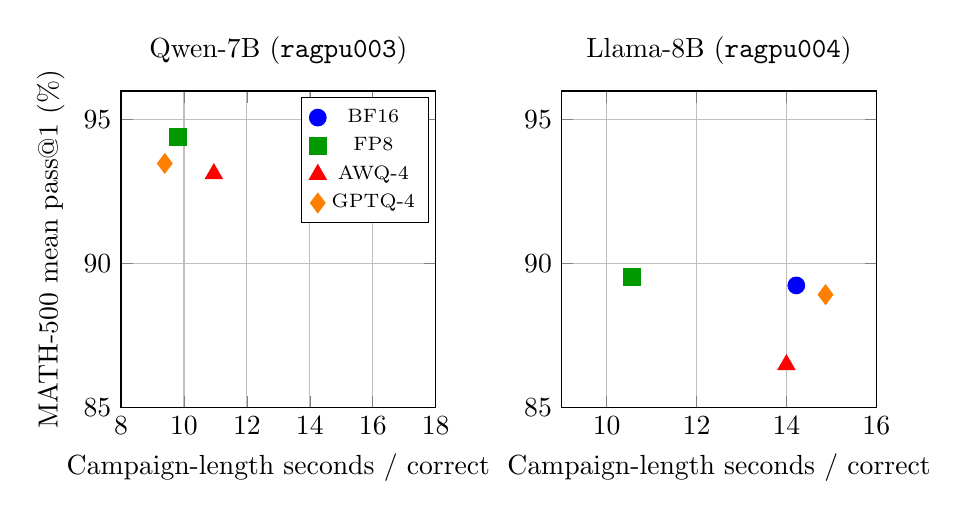
\begin{tikzpicture}
\begin{groupplot}[
    group style={
        group size=2 by 1,
        horizontal sep=1.6cm,
        ylabels at=edge left,
    },
    width=0.46\linewidth, height=5.6cm,
    xlabel={Campaign-length seconds / correct},
    ylabel={MATH-500 mean pass@1 (\%)},
    ymin=85, ymax=96,
    grid=major,
    legend style={font=\scriptsize},
]
\nextgroupplot[title={Qwen-7B (\texttt{ragpu003})}, xmin=8, xmax=18]
\addplot[only marks, mark=*, blue, mark size=3pt] coordinates {(16.89,94.00)};
\addplot[only marks, mark=square*, green!60!black, mark size=3pt] coordinates {(9.82,94.40)};
\addplot[only marks, mark=triangle*, red, mark size=3.5pt] coordinates {(10.95,93.12)};
\addplot[only marks, mark=diamond*, orange, mark size=3.5pt] coordinates {(9.39,93.48)};
\legend{BF16, FP8, AWQ-4, GPTQ-4}
\nextgroupplot[title={Llama-8B (\texttt{ragpu004})}, xmin=9, xmax=16]
\addplot[only marks, mark=*, blue, mark size=3pt] coordinates {(14.22,89.24)};
\addplot[only marks, mark=square*, green!60!black, mark size=3pt] coordinates {(10.56,89.52)};
\addplot[only marks, mark=triangle*, red, mark size=3.5pt] coordinates {(14.00,86.48)};
\addplot[only marks, mark=diamond*, orange, mark size=3.5pt] coordinates {(14.87,88.92)};
\end{groupplot}
\end{tikzpicture}
\caption{Campaign-length seconds per correct answer versus MATH-500 pass@1. The horizontal axis is full-grid mean tokens divided by the measured Condition~B tok/s (total tokens over total time) and by pass@1. There are no timing whiskers: $R=3$ or $5$ does not support a percentile interval, and those repeats do not resample length. Points are not joined. Panels are separate hosts and are not a pooled trade-off plot.}
\label{fig:condB-scatter}
\end{figure}

\FloatBarrier
\section{Agreement detail}
\label{app:modal}
The compact recovered artifact has 20{,}000 rows (SHA256 prefix \texttt{23e9ead021111959}; full digest is in the JSON sidecar). It stores extracted prediction representations, campaign \path{extractive_match}, and completion tokens. It does not store chain-of-thought or problem text. Campaign extraction used LightEval~0.8.0. Campaign extractive match was reproduced on 20{,}000/20{,}000 rows before clustering. Equivalence clustering reported 0 symmetry violations, 0 transitivity violations, and 116 non-unique-mode ties among 4{,}000 groups. Bootstrap uses $B=10{,}000$ problem resamples with seed $20260816$. Secondary ECE/Brier scores (confidence $=m_i/5$) are in the JSON report and are not treated as a primary calibration result.

$T_5$ is the five-sample token-cost proxy: the sum of completion tokens over seeds 42--46. Mean / median / P90 $T_5$ are computed over all 500 items. Tokens per served query and tokens per correct served result use that same 500-item $T_5$ total in the numerator, so abstained queries are not free.

\begin{table}[!htbp]
\centering
\caption{Observable modal-answer agreement on MATH-500 ($n=500$, seeds 42--46). Coverage is the fraction of items with a unique modal class of size $\ge k$. Risk is $1-$selective accuracy among served items. Mean $T_5$ is the five-sample token-cost proxy over all 500 items (abstained queries still pay). Gold is used only to score served predictions.}
\label{tab:modal}
\small
\resizebox{\textwidth}{!}{%
\begin{tabular}{llccccccc}
\toprule
\textbf{Model} & \textbf{Fmt} & $\ge$3/5 cov. & $\ge$3/5 risk & $\ge$4/5 cov. & $\ge$4/5 risk & 5/5 cov. & 5/5 risk & Mean $T_5$ \\
\midrule
Qwen-7B & BF16   & 96.0 & 1.67 & 93.4 & 0.43 & 88.4 & 0.23 & 20{,}057 \\
Qwen-7B & FP8    & 96.6 & 1.66 & 92.6 & 0.00 & 88.8 & 0.00 & 20{,}038 \\
Qwen-7B & AWQ-4  & 95.8 & 1.46 & 91.2 & 0.44 & 86.4 & 0.23 & 21{,}327 \\
Qwen-7B & GPTQ-4 & 95.4 & 1.47 & 92.8 & 0.43 & 86.8 & 0.00 & 21{,}436 \\
\midrule
Llama-8B & BF16   & 94.0 & 2.98 & 87.8 & 0.68 & 76.2 & 0.26 & 23{,}283 \\
Llama-8B & FP8    & 94.0 & 3.19 & 88.6 & 0.90 & 78.2 & 0.00 & 22{,}754 \\
Llama-8B & AWQ-4  & 93.2 & 3.65 & 84.6 & 1.89 & 70.2 & 0.00 & 23{,}682 \\
Llama-8B & GPTQ-4 & 93.8 & 2.77 & 86.4 & 0.46 & 75.4 & 0.27 & 24{,}203 \\
\bottomrule
\end{tabular}%
}
\end{table}

\begin{table}[!htbp]
\centering
\caption{Paired coverage $\Delta$ versus matched BF16 (percentage points). Intervals that exclude zero are marked $^*$. Selective-accuracy $\Delta$ intervals are in the machine-readable modal report.}
\label{tab:modal-paired}
\small
\begin{tabular}{llccc}
\toprule
\textbf{Contrast} & $\ge$3/5 cov.\ $\Delta$ [95\% CI] & $\ge$4/5 cov.\ $\Delta$ [95\% CI] & 5/5 cov.\ $\Delta$ [95\% CI] \\
\midrule
Qwen FP8     & $+0.6\ [-0.8,+2.0]$ & $-0.8\ [-2.2,+0.6]$ & $+0.4\ [-1.6,+2.4]$ \\
Qwen AWQ-4   & $-0.2\ [-1.8,+1.2]$ & $-2.2\ [-4.0,-0.6]^*$ & $-2.0\ [-4.4,+0.2]$ \\
Qwen GPTQ-4  & $-0.6\ [-2.0,+0.8]$ & $-0.6\ [-2.2,+1.0]$ & $-1.6\ [-4.2,+0.8]$ \\
Llama FP8    & $0.0\ [-1.8,+1.8]$ & $+0.8\ [-1.6,+3.2]$ & $+2.0\ [-1.2,+5.2]$ \\
Llama AWQ-4  & $-0.8\ [-2.8,+1.2]$ & $-3.2\ [-6.0,-0.6]^*$ & $-6.0\ [-9.4,-2.6]^*$ \\
Llama GPTQ-4 & $-0.2\ [-2.2,+1.8]$ & $-1.4\ [-3.8,+1.0]$ & $-0.8\ [-4.2,+2.6]$ \\
\bottomrule
\end{tabular}
\end{table}

\begin{sidewaystable}
\centering
\caption{Cost curve for $k$-sample unanimity on MATH-500. Coverage (Cov.) and selective risk (Risk) are averaged over all $\binom{5}{k}$ seed subsets. Len.: one-sample shortest-trace rule at the same coverage, averaged over five seeds. Tokens per item are $k$ times the mean completion length. The $k=5$ column reproduces the 5/5 columns of Tables~\ref{tab:modal} and~\ref{tab:length-abstain} except two entries that share one cause, a single item in Qwen GPTQ-4: coverage ($86.6$ here, $86.8$ there) and the matched-coverage length-rule risk ($1.62$ here, $1.61$ there). All values are percentages except tokens.}
\label{tab:kcurve}
\small
\begin{tabular}{llcccccccccccc}
\toprule
 & & \multicolumn{3}{c}{$k=2$} & \multicolumn{3}{c}{$k=3$} & \multicolumn{3}{c}{$k=4$} & \multicolumn{3}{c}{$k=5$} \\
\cmidrule(lr){3-5}\cmidrule(lr){6-8}\cmidrule(lr){9-11}\cmidrule(lr){12-14}
\textbf{Model} & \textbf{Fmt} & Cov. & Risk & Len. & Cov. & Risk & Len. & Cov. & Risk & Len. & Cov. & Risk & Len. \\
\midrule
Qwen-7B & BF16   & 92.5 & 0.89 & 2.20 & 90.7 & 0.44 & 1.94 & 89.4 & 0.27 & 1.83 & 88.4 & 0.23 & 1.67 \\
Qwen-7B & FP8    & 92.7 & 0.69 & 2.16 & 90.7 & 0.18 & 1.94 & 89.6 & 0.00 & 1.88 & 88.8 & 0.00 & 1.71 \\
Qwen-7B & AWQ-4  & 91.2 & 1.05 & 2.54 & 88.8 & 0.43 & 2.34 & 87.4 & 0.27 & 2.15 & 86.4 & 0.23 & 1.99 \\
Qwen-7B & GPTQ-4 & 91.6 & 0.87 & 2.31 & 89.3 & 0.29 & 1.92 & 87.8 & 0.09 & 1.69 & 86.6 & 0.00 & 1.62 \\
\midrule
Llama-8B & BF16   & 85.8 & 1.86 & 4.06 & 81.5 & 0.71 & 3.34 & 78.5 & 0.36 & 3.16 & 76.2 & 0.26 & 2.83 \\
Llama-8B & FP8    & 86.9 & 1.91 & 4.47 & 82.9 & 0.63 & 3.82 & 80.3 & 0.20 & 3.39 & 78.2 & 0.00 & 3.17 \\
Llama-8B & AWQ-4  & 82.1 & 2.36 & 5.84 & 76.8 & 1.07 & 4.90 & 73.1 & 0.44 & 4.71 & 70.2 & 0.00 & 4.56 \\
Llama-8B & GPTQ-4 & 85.1 & 1.76 & 4.08 & 80.5 & 0.62 & 3.03 & 77.6 & 0.31 & 2.78 & 75.4 & 0.27 & 2.55 \\
\midrule
\multicolumn{2}{l}{Tokens / item (Qwen; Llama)} & \multicolumn{3}{c}{$\approx 8.0$--$8.6$k; $9.1$--$9.7$k} & \multicolumn{3}{c}{$\approx 12.0$--$12.9$k; $13.7$--$14.5$k} & \multicolumn{3}{c}{$\approx 16.0$--$17.1$k; $18.2$--$19.4$k} & \multicolumn{3}{c}{$\approx 20.0$--$21.4$k; $22.8$--$24.2$k} \\
\bottomrule
\end{tabular}
\end{sidewaystable}

\begin{table}[!htbp]
\centering
\caption{One-sample length abstention at the published 5/5 coverage. For each seed, serve the shortest $k$ traces. Risk is the mean over seeds 42--46. Modal risk is the 5/5 column of Table~\ref{tab:modal}.}
\label{tab:length-abstain}
\small
\begin{tabular}{llccc}
\toprule
\textbf{Model} & \textbf{Fmt} & $k$ & \textbf{Length risk (\%)} & \textbf{5/5 modal risk (\%)} \\
\midrule
Qwen-7B & BF16 & 442 & 1.67 & 0.23 \\
Qwen-7B & FP8 & 444 & 1.71 & 0.00 \\
Qwen-7B & AWQ-4 & 432 & 1.99 & 0.23 \\
Qwen-7B & GPTQ-4 & 434 & 1.61 & 0.00 \\
Llama-8B & BF16 & 381 & 2.83 & 0.26 \\
Llama-8B & FP8 & 391 & 3.17 & 0.00 \\
Llama-8B & AWQ-4 & 351 & 4.56 & 0.00 \\
Llama-8B & GPTQ-4 & 377 & 2.55 & 0.27 \\
\bottomrule
\end{tabular}
\end{table}

\begin{table}[!htbp]
\centering
\caption{Adaptive agreement sampling on MATH-500. Each entry is coverage (\%) / selective risk (\%) / mean tokens per item (thousands). Fixed $\ge 3/5$: the five-sample rule of Table~\ref{tab:modal}. Adaptive: draw two samples and serve if they agree; otherwise draw three more and serve the unique mode only if it has at least three of the five votes. Fixed $k{=}2$: unanimity of two samples (Table~\ref{tab:kcurve}). Adaptive and fixed $k{=}2$ are averaged over all 120 orderings of the five stored seeds, with the realised tokens of the samples drawn; item-level bootstrap intervals are in \texttt{results/reports/adaptive\_reflection\_rope.json}. No parameter was fitted to these data. From \texttt{scripts/analysis/adaptive\_reflection\_rope.py}.}
\label{tab:adaptive}
\small
\begin{tabular}{llll}
\toprule
\textbf{Cell} & \textbf{Fixed $\ge 3/5$} & \textbf{Adaptive} & \textbf{Fixed $k{=}2$} \\
\midrule
Qwen BF16 & 96.0 / 1.67 / 20.1 & 96.3 / 1.72 / 10.9 & 92.5 / 0.89 / 8.0 \\
Qwen FP8 & 96.6 / 1.66 / 20.0 & 96.8 / 1.71 / 10.7 & 92.7 / 0.69 / 8.0 \\
Qwen AWQ-4 & 95.8 / 1.46 / 21.3 & 96.2 / 1.77 / 11.9 & 91.2 / 1.05 / 8.5 \\
Qwen GPTQ-4 & 95.4 / 1.47 / 21.4 & 95.7 / 1.65 / 11.9 & 91.6 / 0.87 / 8.6 \\
\midrule
Llama BF16 & 94.0 / 2.98 / 23.3 & 94.5 / 3.34 / 14.0 & 85.8 / 1.86 / 9.3 \\
Llama FP8 & 94.0 / 3.19 / 22.8 & 94.5 / 3.47 / 13.3 & 86.9 / 1.91 / 9.1 \\
Llama AWQ-4 & 93.2 / 3.65 / 23.7 & 93.6 / 4.06 / 15.0 & 82.1 / 2.36 / 9.5 \\
Llama GPTQ-4 & 93.8 / 2.77 / 24.2 & 94.4 / 3.18 / 14.7 & 85.1 / 1.76 / 9.7 \\
\bottomrule
\end{tabular}
\end{table}

\begin{figure}[!htbp]
\centering
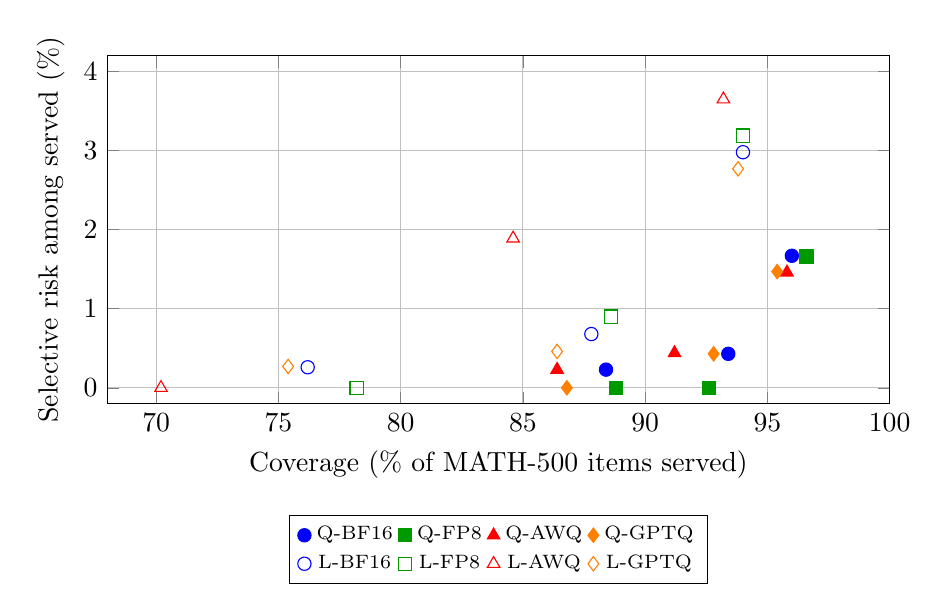
\begin{tikzpicture}
\begin{axis}[
    width=0.95\linewidth, height=6.0cm,
    xlabel={Coverage (\% of MATH-500 items served)},
    ylabel={Selective risk among served (\%)},
    xmin=68, xmax=100,
    ymin=-0.2, ymax=4.2,
    grid=major,
    legend columns=4,
    legend style={font=\scriptsize, at={(0.5,-0.32)}, anchor=north},
]
\addplot[only marks, mark=*, blue, mark size=2.4pt] coordinates {(96.0,1.67)(93.4,0.43)(88.4,0.23)};
\addplot[only marks, mark=square*, green!60!black, mark size=2.4pt] coordinates {(96.6,1.66)(92.6,0.00)(88.8,0.00)};
\addplot[only marks, mark=triangle*, red, mark size=2.6pt] coordinates {(95.8,1.46)(91.2,0.44)(86.4,0.23)};
\addplot[only marks, mark=diamond*, orange, mark size=2.6pt] coordinates {(95.4,1.47)(92.8,0.43)(86.8,0.00)};
\addplot[only marks, mark=o, blue, mark size=2.4pt] coordinates {(94.0,2.98)(87.8,0.68)(76.2,0.26)};
\addplot[only marks, mark=square, green!60!black, mark size=2.4pt] coordinates {(94.0,3.19)(88.6,0.90)(78.2,0.00)};
\addplot[only marks, mark=triangle, red, mark size=2.6pt] coordinates {(93.2,3.65)(84.6,1.89)(70.2,0.00)};
\addplot[only marks, mark=diamond, orange, mark size=2.6pt] coordinates {(93.8,2.77)(86.4,0.46)(75.4,0.27)};
\legend{Q-BF16, Q-FP8, Q-AWQ, Q-GPTQ, L-BF16, L-FP8, L-AWQ, L-GPTQ}
\end{axis}
\end{tikzpicture}
\caption{Three discrete MATH-500 operating points ($\ge 3/5$, $\ge 4/5$, $5/5$), not a continuous risk--coverage curve. Filled markers: Qwen-7B. Open markers: Llama-8B. Lower-right is the preferred corner (high coverage, low risk); the $\ge 3/5$ points sit at the upper right (high coverage, higher risk) and the 5/5 points at the lower left (strict consensus, lower coverage).}
\label{fig:modal}
\end{figure}

\FloatBarrier
\section{Neighboring measurement studies}
\label{app:related}
Table~\ref{tab:related} is a compact comparison of designs; it is not a claim that this paper replaces those studies.

\begin{table}[!htbp]
\centering
\caption{Neighboring measurement studies. In the engine column, a named version means that serving stack is frozen while checkpoints vary. Length estimands and serving columns are what each paper reports as primary evidence, not an exhaustive inventory.}
\label{tab:related}
\footnotesize
\setlength{\tabcolsep}{4pt}
\renewcommand{\arraystretch}{1.15}
\begin{tabularx}{\textwidth}{@{}>{\raggedright\arraybackslash}p{0.14\textwidth}*{4}{>{\raggedright\arraybackslash}X}@{}}
\toprule
\textbf{Study} & \textbf{Models; bits} & \textbf{Engine; seeds} & \textbf{Length estimand; correctness split} & \textbf{Serving / cost; statistics} \\
\midrule
This paper & 2 R1 distill (7B/8B); BF16, FP8, AWQ-4, GPTQ-4 & vLLM 0.7.0 eager, A100; 5 seeds MATH, 3 GSM/GPQA & RoM, paired $\Delta$, both conditionals, seed placebo; $2\times 2$ + both mirrors & GPU-s, campaign-length seconds; item-level bootstrap, Holm, TOST \\
QRM~\cite{liu2025qrm} & R1 distill family; W/A/KV incl.\ W4A16 & QRM harness (multi-config); 3 seeds (v2) & mean tokens; not $2\times 2$ & limited; per-cell means \\
Lian et al.~\cite{lian2026quantinflates} & reasoning models; low-bit PTQ & paper stack; greedy ($T=0$), 100 questions per benchmark, one seed & CTIR (ratio of mean CoT-only lengths); BF16-correct vs rest (suppl.) & token cost; length ratio \\
Lotfi et al.~\cite{lotfi2026overthinking} & 1.5B--32B reasoning; aggressive PTQ & paper stack; paper-specific seeds & CoT length, overthinking; abandoned intermediates & logit-penalty Pareto; error-type counts \\
Kurtic et al.~\cite{kurtic2025give} & Llama-3.1 + R1-distill; FP8/INT8/INT4 & vLLM, several GPUs; large evals & not CoT-primary; N/A & sync vs continuous batching; accuracy + tok/s \\
Helcig et al.~\cite{helcig2026slq} & Llama/Qwen (SLQ); 3.3--6 bpp & vLLM kernels; 3 seeds (GSM) & thinking tokens; TL vs DL fidelity & vLLM throughput; EAR, Wilcoxon \\
Erol et al.~\cite{erol2025costofpass} & general LMs; N/A & N/A & N/A & $C_{\mathrm{pass}}$ definition; economic \\
Hochlehnert et al.~\cite{hochlehnert2025sober} & reasoning LMs; N/A & deliberately \emph{un}pinned; many seeds & N/A & N/A; reproducibility \\
\bottomrule
\end{tabularx}
\end{table}

\FloatBarrier
\section{Follow-up experiments: protocol, checks and deviations}
\label{app:followup}
The follow-up experiments of Section~\ref{sec:followup} and the self-quantized AWQ-4 checkpoint of Section~\ref{sec:res1} comprise 48 cells and 26{,}457 completions (E1: five MATH-500 and three GSM8K cells, plus five E1c cells; E2, E3 and X1: ten cells each; X3: five cells), generated after the campaign on the same A100 stack with a copy of the campaign code whose launcher was changed only to add an output-file suffix, a temperature override, a quantization-kernel override and a dump of the engine's effective settings.

\paragraph{Configuration.} All cells use the campaign prompts, vLLM~0.7.0 in eager mode, \texttt{max\_model\_len} and maximum new tokens of $32{,}768$, top-$p$ $0.95$ and the campaign seeds (42--46; 42--44 on GSM8K; 47--51 for X1), with $T=0.6$ except E3 ($T=0.8$). E2 loads the BF16 weights with \texttt{dtype=float16}. E1 uses a checkpoint quantized by AutoAWQ~0.2.9 with 4-bit weights, group size 128, \texttt{zero\_point=True}, GEMM packing and Pile-validation calibration; the quantization job validated the configuration, loaded the model in vLLM, and produced 50 prompts byte-identical to the campaign's. vLLM resolved this checkpoint to the AWQ-Marlin kernel, whereas the community uploads (\texttt{zero\_point=false}) run on the GEMM kernel; activations are \texttt{float16} in both.

\paragraph{Checks.} The first cell of each job had to pass a gate before the job continued: prompts byte-identical to the campaign's, the same record schema, a complete stop-reason log, and, from the live engine object after loading, the effective dtype, quantization kernel, \texttt{max\_num\_seqs} ($256$, the vLLM~0.7.0 default used by the campaign), eager mode, and no prefix caching or chunked prefill. The expected values were written before any rerun finished. All 48 cells are recorded as passing in the cell-status file. The gate itself ran on seed 42 of each job; later seeds carry the per-cell verification only, and the gate script prints ``token offset 0'' because that text is hard-coded, although the jobs were launched expecting an offset of $+1$.

\paragraph{Doubled beginning-of-sequence token.} The first gate flagged one more prompt token in the engine than the frozen-tokenizer recount on all 500 rows of the first rerun cell (for example $44$ against $43$ tokens for item~0 of Qwen). The prompt string already begins with the beginning-of-sequence token and the pipeline's default \texttt{add\_special\_tokens=True} adds another; tokenizing item~0 with and without special tokens reproduces both counts for both families ($44/43$ Qwen, $40/39$ Llama). We did not store engine prompt lengths in the campaign. The relation between completion length and the recount at the output cap is the same in the reruns as in the campaign, which we take as evidence that the campaign engine received the same doubled token; the gate was therefore set to expect an offset of exactly $+1$ on every row, and any other offset fails. We did not test whether the extra token affects results.

\paragraph{Pre-registered rules and their outcome.} Written before the data existed: E1, an interval for the accuracy drop that excludes zero means the drop is a property of AWQ-4 on this stack and not of the community upload (met on MATH-500 and GSM8K); E3, a positive $\Lambda_b$ with a null excess means the placebo generalizes beyond quantization (met for Llama, not for Qwen); X1, the interval of $\Pi_b^{\mathrm{new}}-\Pi_b^{\mathrm{old}}$ contains zero for both families (met). Rules for E1c and X3 were written after E1--E3 and X1 were analysed and before any E1c or X3 cell had finished (in a file committed to the released repository): E1c, the accuracy interval excludes zero (met), and the length excess, estimated with cross-seed pairs as that file specifies, is kernel-robust if its interval excludes zero or kernel-dependent if it includes zero while the paired difference from the Marlin excess excludes zero (kernel-robust: the cross-seed excess is $+172$ $[+23,+323]$, against $+119$ $[-32,+270]$ with seed-matched pairs; an earlier version of our analysis applied this rule to seed-matched pairs and reported it as inconclusive, which departed from the specified estimator); X3, the cross-seed excess is consistent with the placebo if its interval includes zero (met: $+111$ $[-14,+241]$). The first version of the X1 rule compared the new placebo with the plug-in selection term, which by the identity $\Pi_b=\tfrac{m}{m-1}\widehat S_b$ carries a built-in $25\%$ offset for $m=5$; it was corrected before any X1 data existed. The length excess for E1, the comparisons against the ten-seed placebo, the per-level breakdown and the self-AWQ versus upload contrast are exploratory.

\paragraph{Cross-seed pairing.} Using all cross-seed pairs instead of seed-matched pairs changes each follow-up $\Lambda_b$ by at most $53$ tokens (E1c: $+355$ seed-matched, $+407$ cross-seed). The excess interval changes in whether it contains zero for two contrasts: E1c (excludes zero with cross-seed pairs, not with seed-matched pairs) and X3 (the reverse, $+111$ $[-14,+241]$ cross-seed against $+136$ $[+2,+274]$ seed-matched); every other contrast of E1--E3 is unchanged. We did not compute cross-seed versions for the companion-study cells.

\paragraph{Cells from companion studies.} Section~\ref{sec:artifacts} and Table~\ref{tab:p4ctrl} use cells produced by separate studies on the same stack and cluster; the repository's documents label the first set publication-phase and the second pilot-only. They are $36$ cells with Qwen-7B checkpoints that we quantized (three calibration draws $\times$ three seeds for each of GPTQ-4 and AWQ-4, on MATH-500 and on GSM8K), $18$ \texttt{float16} control cells for GPTQ-4 (nine per benchmark), and $33$ decoding-grid cells (eleven settings of temperature, token budget and format $\times$ three seeds, on $300$ MATH-500 items). These runs stored exact-match scores, which are far below the campaign's; we rescored the stored completions with the campaign's own scoring functions (LightEval~0.8.0 metric objects) after checking that the rescoring reproduces the stored campaign scores on all $500$ MATH-500 rows and on all $1{,}319$ rows of the E1 GSM8K cells. Rows were matched to the campaign's through the dataset item identifier (the GSM8K order differs between the two sets and was joined on the dataset index). Compared with the E2 cells, which use the campaign pipeline, the prompts of the P2 cells and of the AWQ-4 cells of the decoding grid have exactly one token fewer on every MATH-500 item (a single instead of a doubled beginning-of-sequence token), while the BF16 cells of the decoding grid have identical prompts; the corresponding check was not possible for GSM8K, where no campaign-pipeline prompt lengths are stored. We report descriptive contrasts against the campaign BF16 cells only; none of those studies' own primary endpoints is used.

% generated by analysis/gen_p2p4_tables.py -- do not edit by hand
\begin{table}[t]
\centering
\caption{Real changes to the sampling setting, as positive controls for the placebo (Qwen-7B, 300 MATH-500 items, seeds 42--44, seed-matched pairs; tokens; item-level 95\% intervals). Reference: the campaign BF16 cells at $T=0.6$ and a 32{,}768-token budget on the same items; the five-seed placebo on these items is $+121$ $[+47,+208]$. Settings differ in temperature $T$ and maximum new tokens (8k = 8{,}192, 32k = 32{,}768). The last column is the share of completions that stopped at the length limit. Pilot grid with one engine setting per cell; AWQ-4 is a self-quantized checkpoint on the GEMM kernel at \texttt{float16}. $^{\dagger}$The prompts of the AWQ-4 cells lack the campaign's doubled beginning-of-sequence token (one token fewer on every item); the BF16 rows use exactly the campaign's prompts.}
\label{tab:p4ctrl}
\small
\resizebox{\linewidth}{!}{%
\begin{tabular}{lccccc}
\toprule
\textbf{Setting} & \vcell{\textbf{pass@1}}{$\Delta$ (pp)} & \vcell{\textbf{Unconditional}}{$\overline{\Delta\ell}$} & \vcell{\textbf{BF16-correct}}{$\Lambda_b$} & \vcell{\textbf{Excess}}{$\Lambda_b-\Pi_b$} & \textbf{Stops} \\
\midrule
BF16, $T=0.2$, 32k & \vcell{$-4.56$}{$[-6.56,-2.67]$} & \vcell{$+1534$}{$[+973,+2163]$} & \vcell{$+1191$}{$[+705,+1719]$} & \vcell{$+1070$}{$[+591,+1596]$} & 8.6\% \\
BF16, $T=1.0$, 32k & \vcell{$-1.22$}{$[-3.00,+0.56]$} & \vcell{$+172$}{$[-64,+393]$} & \vcell{$+384$}{$[+195,+575]$} & \vcell{$+263$}{$[+86,+435]$} & 0.0\% \\
BF16, $T=0.6$, 8k & \vcell{$-4.11$}{$[-6.11,-2.11]$} & \vcell{$-710$}{$[-1047,-406]$} & \vcell{$-284$}{$[-478,-112]$} & \vcell{$-406$}{$[-613,-217]$} & 9.0\% \\
BF16, $T=0.2$, 8k & \vcell{$-6.56$}{$[-8.89,-4.44]$} & \vcell{$-755$}{$[-1091,-447]$} & \vcell{$-371$}{$[-572,-190]$} & \vcell{$-492$}{$[-708,-294]$} & 12.4\% \\
BF16, $T=1.0$, 8k & \vcell{$-4.00$}{$[-6.00,-2.00]$} & \vcell{$-403$}{$[-749,-93]$} & \vcell{$+26$}{$[-181,+208]$} & \vcell{$-95$}{$[-315,+102]$} & 10.0\% \\
\midrule
Self-quantized AWQ-4$^{\dagger}$, $T=0.6$, 32k & \vcell{$-1.22$}{$[-2.67,+0.11]$} & \vcell{$-120$}{$[-346,+101]$} & \vcell{$+5$}{$[-185,+200]$} & \vcell{$-117$}{$[-307,+76]$} & 0.9\% \\
AWQ-4$^{\dagger}$, $T=0.2$, 32k & \vcell{$-5.22$}{$[-7.67,-3.00]$} & \vcell{$+1553$}{$[+1007,+2142]$} & \vcell{$+1475$}{$[+938,+2062]$} & \vcell{$+1354$}{$[+818,+1932]$} & 9.0\% \\
AWQ-4$^{\dagger}$, $T=1.0$, 32k & \vcell{$-1.67$}{$[-3.44,0.00]$} & \vcell{$-111$}{$[-379,+159]$} & \vcell{$+120$}{$[-103,+356]$} & \vcell{$-2$}{$[-222,+227]$} & 0.0\% \\
AWQ-4$^{\dagger}$, $T=0.6$, 8k & \vcell{$-5.11$}{$[-7.22,-3.22]$} & \vcell{$-806$}{$[-1143,-506]$} & \vcell{$-398$}{$[-592,-224]$} & \vcell{$-519$}{$[-731,-332]$} & 9.9\% \\
AWQ-4$^{\dagger}$, $T=0.2$, 8k & \vcell{$-7.67$}{$[-10.33,-5.22]$} & \vcell{$-786$}{$[-1134,-471]$} & \vcell{$-366$}{$[-573,-174]$} & \vcell{$-488$}{$[-712,-282]$} & 13.0\% \\
AWQ-4$^{\dagger}$, $T=1.0$, 8k & \vcell{$-5.33$}{$[-7.78,-3.11]$} & \vcell{$-664$}{$[-1006,-355]$} & \vcell{$-246$}{$[-447,-63]$} & \vcell{$-367$}{$[-583,-173]$} & 10.3\% \\
\bottomrule
\end{tabular}%
}
\end{table}


\paragraph{Deviations in the records.}
(i) The first attempt at E2 and E3 stopped at the first cell because the checker read an engine start-up line that vLLM~0.7.0 does not write to the cell log; it was replaced by direct reading of the engine settings, a second checker fault (it read the wrong record file) was fixed, and the earlier outputs are kept separately and excluded from every number here. The affected status rows are marked as superseded, with the originals preserved. The Qwen \texttt{float16} seed-42 cell was generated three times (the two discarded runs and the counted run); the three outputs are byte-identical ($500$ of $500$ items token-identical, pass@1 $94.8$ in all), so a repeat at the same seed and configuration adds no noise here and the exclusion costs nothing. This is one cell and does not show that every configuration is deterministic.
(ii) The five MATH-500 cells and the three GSM8K cells of E1 share one output directory per seed. The GSM8K runs overwrote the raw output, stop-reason sidecar and engine dump of the MATH-500 cells for seeds 42--44. The per-item records and status rows of those three cells survive, so they lack stop reasons and an individual engine dump; their configuration is that of the job, whose engine dump is present for seeds 45--46 and for the GSM8K cells.
(iii) In 32 rows across the cells, the engine's completion-token count and the stored count differ by more than two tokens. No analysis uses the engine count.
(iv) The comparison cells are the campaign BF16 cells from the original runs, not new BF16 cells run in the same jobs.

\section{Detailed limitations and threats to validity}
\label{app:limitations}
\begin{enumerate}
    \item \textbf{A100 W8A16 fallback.} FP8 checkpoints were executed as Marlin W8A16 on A100, not native W8A8. Numbers do not transfer to Hopper native W8A8.
    \item \textbf{Measured serving scope.} Throughput and GPU-seconds are measured on balanced MATH-500 subsets, not the full campaign. Repeats share one sampling seed, so cost intervals omit length variance. Condition~B elapsed time includes the straggler tail; occupancy time was not stored. $R=3$ or $5$ does not support a stable percentile interval. Eager execution was not compared with CUDA graphs. Qwen and Llama used different hosts. Formats ran sequentially on non-exclusive nodes, and clocks and co-tenant load were not logged. The Qwen BF16 baseline appears slow, which alone would bias the Qwen savings upward, but the quantized runs may also have been affected by changing conditions (the FP8 Condition~B repeats step up in run order), so the direction of the net bias is unknown. The timer's prompts carry one more input token per request than the frozen-tokenizer recount, as do the campaign's (a doubled beginning-of-sequence token, Appendix~\ref{app:followup}). The $\$1.50$/A100-hour rate is a pricing scenario. Peak VRAM is the $0.75$ engine pool.
    \item \textbf{Activation dtype.} AWQ-4 accuracy runs use \texttt{float16}. BF16, FP8, and accuracy-campaign GPTQ-4 use \texttt{bfloat16}. Serving GPTQ-4 uses \texttt{float16}. A BF16-at-\texttt{float16} control was run afterwards for MATH-500 (Section~\ref{sec:followup}); the GSM8K and GPQA-Diamond cells have none.
    \item \textbf{Pathology metrology.} The loop detector is identical-word runs $\ge 20$. Phrase-level cycles and \texttt{finish\_reason} were not saved. Truncation is measured by a per-item cap band (within 16 tokens of the cap implied by the stored prompt), not by a native stop reason. GPQA letter order was a process-RNG draw; the stored prompts show it was identical across checkpoints and across the three generation seeds, so every GPQA number is conditional on one answer-letter permutation and position bias does not average out across seeds.
    \item \textbf{Item order.} Compact JSON rows follow the campaign pipeline order. All paired analyses are within that order and are unaffected: the eight cells agree item by item. Joins against public per-item metadata (difficulty level) use exact question text from the stored campaign prompts; all 500 rows match distinct dataset items in both families.
    \item \textbf{Modal agreement.} Five generations are required per attempted MATH problem. Only MATH-500 has five seeds in this campaign. Mathematical answer equivalence is evaluator- and task-specific (campaign LightEval~0.8.0 / math-verify). High agreement can still be wrong. The signal is not general uncertainty calibration, not softmax calibration, and not a safety property. The one-sample length rule is a weak comparator; token-level confidence (mean log-probability, self-certainty) was not stored, so the stronger gold-free comparison is not made.
    \item \textbf{Checkpoint provenance.} Both AWQ-4 checkpoints are \texttt{jakiAJK} uploads with unknown calibration. FP8 and GPTQ-4 are RedHatAI artifacts. The configurations suggest an AutoRound-style symmetric export in AWQ format (Section~\ref{sec:formats}). Format, publisher, toolchain, activation dtype, AWQ kernel path, and chat template are collinear. A second Llama AWQ-4 artifact was quantized afterwards by the authors (Section~\ref{sec:res1}), and three calibration draws each of Qwen GPTQ-4 and AWQ-4 were quantized by a companion study (Section~\ref{sec:artifacts}).
    \item \textbf{Scope.} Two 7--8B DeepSeek-R1 distillations, English math/science, one pinned serving stack, one prompt. GSM8K/GPQA use three seeds.
    \item \textbf{Not evaluated.} This study does not evaluate AIME, LiveCodeBench, 32B models, Hopper native W8A8 FP8, energy measurements, production continuous batching, or probability calibration.
    \item \textbf{Reproducibility surface.} Compact JSON, recovered MATH-500 answer strings, confirmation timing, and analysis reports are released. Full chain-of-thought traces are not. Compact JSON omits \texttt{finish\_reason} and output token IDs. Replay needs an A100-80GB, the listed weights, and \path{runtime_manifest.json}. The serving records log driver 550.54.14; the accuracy-campaign job logs did not archive the driver. Each table and figure maps to its script and output file in \path{docs/PAPER_TO_CODE.md}. Analyses that need completion text (the reflection-marker counts, the frozen-tokenizer recount and exact-cap test, the \texttt{<think>} audit, and the cap-band assignment of the failure classes) run on the authors' archive of completions, which is not released; every other analysis uses only the released records.
    \item \textbf{Contamination.} MATH and GSM8K overlap public pretraining corpora. A paired within-item design reduces but does not eliminate contamination interaction with checkpoint.
    \item \textbf{Launcher record.} Effective flags, including \texttt{max\_model\_len=32768}, are reconstructed in \path{runtime_manifest.json} from the launcher. The engine-initialization logs of the serving jobs confirm the engine version, eager mode, context length, seed, dtype and quantization setting per format; the accuracy-campaign logs contain no engine-initialization line, so its dtype rests on the launcher code, not on a log. The accuracy-campaign NVIDIA driver was not archived; the serving confirmation logs 550.54.14. Historical harness configs are not the campaign stack.
\end{enumerate}

\paragraph{Threats to validity.}
Construct: pass@1, maj@5, token length, subset GPU-seconds, and campaign-length seconds are distinct estimands. The hybrid proxy is not Erol et al.'s per-problem Cost-of-Pass. Internal: Conditions~A and~B differ in subset and regime together; timing repeats do not resample length; Qwen and Llama used different hosts. External: two 7--8B families, one eager A100 stack, and three English benchmarks. Results do not transfer to CUDA-graph serving, Hopper W8A8, or a different publisher's AWQ artifact.

\end{document}
